% Choose the language of your thesis passing 'french' or 'english' as
% \documentclass option.
% Note1: The 'page de garde' will always be written in French.
% Note2: You will have an error if you change the language of the document and
%        compile it without cleaning the auxiliary files. Compiling it again
%        should solve the problem.
\documentclass[english,a4paper,11pt,twoside]{StyleThese}
\newcommand{\included}{}
\usepackage{amsmath,amssymb}             % AMS Math
\usepackage[T1]{fontenc}
\usepackage[utf8x]{inputenc}
\usepackage{babel}
\usepackage{datetime}

\usepackage{lmodern}
\usepackage{tabularx}
%\usepackage{tabular}
\usepackage{multirow}

\usepackage{subfigure}
\usepackage{fancyvrb}
\usepackage{algorithmic}
\usepackage{algorithm}
\usepackage{mathtools}


\usepackage{hhline}
\usepackage[left=1.5in,right=1.3in,top=1.1in,bottom=1.1in,includefoot,includehead,headheight=13.6pt]{geometry}
\renewcommand{\baselinestretch}{1.05}

% Table of contents for each chapter

\usepackage[nottoc, notlof, notlot]{tocbibind}
\usepackage{minitoc}
\setcounter{minitocdepth}{2}
\mtcindent=15pt
% Use \minitoc where to put a table of contents

\usepackage{aecompl}


% Glossary / list of abbreviations

\usepackage[intoc]{nomencl}
\iftoggle{ThesisInEnglish}{%
\renewcommand{\nomname}{Glossary}
}{ %
\renewcommand{\nomname}{Liste des Abréviations}
}

\newcommand{\accom}[1]{\textcolor{red}{[#1]}}

\makenomenclature

% My pdf code

\usepackage{ifpdf}

\ifpdf
  \usepackage[pdftex]{graphicx}
  \DeclareGraphicsExtensions{.jpg}
  \usepackage[a4paper,pagebackref,hyperindex=true]{hyperref}
  \usepackage{tikz}
  \usetikzlibrary{arrows,shapes,calc}
\else
  \usepackage{graphicx}
  \DeclareGraphicsExtensions{.ps,.eps}
  \usepackage[a4paper,dvipdfm,pagebackref,hyperindex=true]{hyperref}
\fi

\graphicspath{{.}{images/}}

%% nicer backref links. NOTE: The flag ThesisInEnglish is used to define the
% language in the back references. Read more about it in These.tex

\iftoggle{ThesisInEnglish}{%
\renewcommand*{\backref}[1]{}
\renewcommand*{\backrefalt}[4]{%
\ifcase #1 %
(Not cited.)%
\or
(Cited in page~#2.)%
\else
(Cited in pages~#2.)%
\fi}
\renewcommand*{\backrefsep}{, }
\renewcommand*{\backreftwosep}{ and~}
\renewcommand*{\backreflastsep}{ and~}
}{%
\renewcommand*{\backref}[1]{}
\renewcommand*{\backrefalt}[4]{%
\ifcase #1 %
(Non cité.)%
\or
(Cité en page~#2.)%
\else
(Cité en pages~#2.)%
\fi}
\renewcommand*{\backrefsep}{, }
\renewcommand*{\backreftwosep}{ et~}
\renewcommand*{\backreflastsep}{ et~}
}

% Links in pdf
\usepackage{color}
\definecolor{linkcol}{rgb}{0,0,0.4} 
\definecolor{citecol}{rgb}{0.5,0,0} 
\definecolor{linkcol}{rgb}{0,0,0} 
\definecolor{citecol}{rgb}{0,0,0}
% Change this to change the informations included in the pdf file

\hypersetup
{
bookmarksopen=true,
pdftitle="Joint Action for Human-Robot Interaction",
pdfauthor="Sandra DEVIN", %auteur du document
pdfsubject="Thesis", %sujet du document
%pdftoolbar=false, %barre d'outils non visible
pdfmenubar=true, %barre de menu visible
pdfhighlight=/O, %effet d'un clic sur un lien hypertexte
colorlinks=true, %couleurs sur les liens hypertextes
pdfpagemode=None, %aucun mode de page
pdfpagelayout=SinglePage, %ouverture en simple page
pdffitwindow=true, %pages ouvertes entierement dans toute la fenetre
linkcolor=linkcol, %couleur des liens hypertextes internes
citecolor=citecol, %couleur des liens pour les citations
urlcolor=linkcol %couleur des liens pour les url
}

% definitions.
% -------------------

\setcounter{secnumdepth}{3}
\setcounter{tocdepth}{2}

% Some useful commands and shortcut for maths:  partial derivative and stuff

\newcommand{\pd}[2]{\frac{\partial #1}{\partial #2}}
\def\abs{\operatorname{abs}}
\def\argmax{\operatornamewithlimits{arg\,max}}
\def\argmin{\operatornamewithlimits{arg\,min}}
\def\diag{\operatorname{Diag}}
\newcommand{\eqRef}[1]{(\ref{#1})}

\usepackage{rotating}                    % Sideways of figures & tables
%\usepackage{bibunits}
%\usepackage[sectionbib]{chapterbib}          % Cross-reference package (Natural BiB)
%\usepackage{natbib}                  % Put References at the end of each chapter
                                         % Do not put 'sectionbib' option here.
                                         % Sectionbib option in 'natbib' will do.
\usepackage{fancyhdr}                    % Fancy Header and Footer

% \usepackage{txfonts}                     % Public Times New Roman text & math font
  
%%% Fancy Header %%%%%%%%%%%%%%%%%%%%%%%%%%%%%%%%%%%%%%%%%%%%%%%%%%%%%%%%%%%%%%%%%%
% Fancy Header Style Options

\pagestyle{fancy}                       % Sets fancy header and footer
\fancyfoot{}                            % Delete current footer settings

%\renewcommand{\chaptermark}[1]{         % Lower Case Chapter marker style
%  \markboth{\chaptername\ \thechapter.\ #1}}{}} %

%\renewcommand{\sectionmark}[1]{         % Lower case Section marker style
%  \markright{\thesection.\ #1}}         %

\fancyhead[LE,RO]{\bfseries\thepage}    % Page number (boldface) in left on even
% pages and right on odd pages
\fancyhead[RE]{\bfseries\nouppercase{\leftmark}}      % Chapter in the right on even pages
\fancyhead[LO]{\bfseries\nouppercase{\rightmark}}     % Section in the left on odd pages

\let\headruleORIG\headrule
\renewcommand{\headrule}{\color{black} \headruleORIG}
\renewcommand{\headrulewidth}{1.0pt}
\usepackage{colortbl}
\arrayrulecolor{black}

\fancypagestyle{plain}{
  \fancyhead{}
  \fancyfoot{}
  \renewcommand{\headrulewidth}{0pt}
}

%\usepackage{MyAlgorithm}
%\usepackage[noend]{MyAlgorithmic}
\usepackage[ED=MITT - STICIA, Ets=INP]{tlsflyleaf}
%%% Clear Header %%%%%%%%%%%%%%%%%%%%%%%%%%%%%%%%%%%%%%%%%%%%%%%%%%%%%%%%%%%%%%%%%%
% Clear Header Style on the Last Empty Odd pages
\makeatletter

\def\cleardoublepage{\clearpage\if@twoside \ifodd\c@page\else%
  \hbox{}%
  \thispagestyle{empty}%              % Empty header styles
  \newpage%
  \if@twocolumn\hbox{}\newpage\fi\fi\fi}

\makeatother
 
%%%%%%%%%%%%%%%%%%%%%%%%%%%%%%%%%%%%%%%%%%%%%%%%%%%%%%%%%%%%%%%%%%%%%%%%%%%%%%% 
% Prints your review date and 'Draft Version' (From Josullvn, CS, CMU)
\newcommand{\reviewtimetoday}[2]{\special{!userdict begin
    /bop-hook{gsave 20 710 translate 45 rotate 0.8 setgray
      /Times-Roman findfont 12 scalefont setfont 0 0   moveto (#1) show
      0 -12 moveto (#2) show grestore}def end}}
% You can turn on or off this option.
% \reviewtimetoday{\today}{Draft Version}
%%%%%%%%%%%%%%%%%%%%%%%%%%%%%%%%%%%%%%%%%%%%%%%%%%%%%%%%%%%%%%%%%%%%%%%%%%%%%%% 

\newenvironment{maxime}[1]
{
\vspace*{0cm}
\hfill
\begin{minipage}{0.5\textwidth}%
%\rule[0.5ex]{\textwidth}{0.1mm}\\%
\hrulefill $\:$ {\bf #1}\\
%\vspace*{-0.25cm}
\it 
}%
{%

\hrulefill
\vspace*{0.5cm}%
\end{minipage}
}

\let\minitocORIG\minitoc
\renewcommand{\minitoc}{\minitocORIG \vspace{1.5em}}

\usepackage{multirow}
%\usepackage{slashbox}

\newenvironment{bulletList}%
{ \begin{list}%
	{$\bullet$}%
	{\setlength{\labelwidth}{25pt}%
	 \setlength{\leftmargin}{30pt}%
	 \setlength{\itemsep}{\parsep}}}%
{ \end{list} }

\newtheorem{definition}{Définition}
\renewcommand{\epsilon}{\varepsilon}

% centered page environment

\newenvironment{vcenterpage}
{\newpage\vspace*{\fill}\thispagestyle{empty}\renewcommand{\headrulewidth}{0pt}}
{\vspace*{\fill}}

\usepackage{tablefootnote}

\sloppy
\begin{document}

%% This is file `example.tex',
%% Copyright 2013 Tristan GREGOIRE
%% Copyright 2015 Yann BACHY
%
% This work may be distributed and/or modified under the
% conditions of the LaTeX Project Public License, either version 1.3
% of this license or (at your option) any later version.
% The latest version of this license is in
%   http://www.latex-project.org/lppl.txt
% and version 1.3 or later is part of all distributions of LaTeX
% version 2005/12/01 or later.
%
%
% This work has the LPPL maintenance status `maintained'.
% 
% The Current Maintainer of this work is T. GREGOIRE
%

%\documentclass{book}

% Loading the tlsflyleaf.sty package require some option to define the
% establishment name, the doctoral school and the PhD speciality.
% In that aim you have 2 key-value option:
%   - Ets=<value> : define the establishment name
%   - ED=<value>  : define the doctoral school and speciality
%   - ED2=<value> : define the second speciality ("double mention"). OPTIONAL.
% The full list of accepted values for each option could be find either
% in the documentation or in ED-list.txt and Ets-list.txt files provide with the package.
%\usepackage[ED=MITT - STICRT, Ets=INSA]{tlsflyleaf}
%\usepackage[ED=SDU2E-Ast, ED2=SDU2E-Eco, Ets=UT3]{tlsflyleaf}

% ==================
% Setup basic string
% - PhD Title
% - author
% - defence date
% - laboratory
% - cotutelle
\title{\textbf{\large Decisional issues during Human-Robot Joint Action}}
\author{Sandra DEVIN}
\defencedate{jj/mm/aaaa}
\lab{Laboratoire d'analyse et d'architecture des systèmes}
%\cotutelle{}

% ==================
% Setup people like your boss, the jury team and the referees
% - First you need to define how number they will be in each category
%   It is done with the commands \nboss{n}, \nreferee{n} and \njudge{n}.
%   You can define more people in each category than the number given 
%   but only the first "\npeople" will be print.
% - Then use the command \makesomeone{<category>}{<number>}{<name>}{<status>}{<other>}
%   where:
%     <category> should be select in ['boss', 'referee', 'judge']
%     <number>   is the rank for printing the person. 
%                Only number <= "\npeople" will be printed
%     <name>     First name and las name of the people
%     <status>   Is (s)he a "charg\'e de recher" ou un "professeur d'universit\'e"...
%     <other>    What ever string you want to add (laboratory, jury member place...).
%% Boss
\nboss{2}
\makesomeone{boss}{2}{Malik Ghallab}{}{}  % Sera affiche en second
\makesomeone{boss}{1}{Rachid ALAMI}{}{} % Sera afiche en premier
%% Referee
\nreferee{2}
\makesomeone{referee}{1}{Peter Ford DOMINEY}{}{}
\makesomeone{referee}{2}{Vanessa Evers}{}{}
%% Judges
\njudge{5}
\makesomeone{judge}{1}{Premier MEMBRE}{Professeur d'Universit\'e}{Pr\'esident du Jury}
\makesomeone{judge}{2}{Second MEMBRE}{Charg\'e de Recherche}{Membre du Jury}
\makesomeone{judge}{3}{Troisi\`eme MEMBRE}{Charg\'e de Recherche}{Membre du Jury}
\makesomeone{judge}{4}{Quatri\`eme MEMBRE}{Charg\'e de Recherche}{Membre du Jury}
\makesomeone{judge}{5}{Ciqui\`eme MEMBRE}{Charg\'e de Recherche}{Membre du Jury}

% ============================================================
% DOCUMENT
%\begin{document}
%    \makeflyleaf
%\end{document}


    \makeflyleaf


\dominitoc

\pagenumbering{roman}

 \cleardoublepage

% Here you can see an example of how to create text conditioned by the language
% variable. The \iftoggle command:
%
%   \iftoggle{ThesisInEnglish}{%
%   <your-text-in-english>
%   }{%
%   <your-text-in-french>
%   }
%
% will compile only one of the two blocks, depending on the variable you set at
% the beginning of this document. Language selection is managed this way in the
% formatAndDefs.tex file. You too can create sections of your thesis that is
% language dependend this way, although you probably won't need it. Another use
% of \iftoggle can be found at the end of this file.
\iftoggle{ThesisInEnglish}{%
\chapter*{Acknowledgments}
}{%
\chapter*{Remerciements}
}

TODO

\ifdefined\included
\else
\documentclass[english,a4paper,11pt,twoside]{StyleThese}
\usepackage{amsmath,amssymb}             % AMS Math
\usepackage[T1]{fontenc}
\usepackage[utf8x]{inputenc}
\usepackage{babel}
\usepackage{datetime}

\usepackage{lmodern}
\usepackage{tabularx}
%\usepackage{tabular}
\usepackage{multirow}

\usepackage{subfigure}
\usepackage{fancyvrb}
\usepackage{algorithmic}
\usepackage{algorithm}
\usepackage{mathtools}


\usepackage{hhline}
\usepackage[left=1.5in,right=1.3in,top=1.1in,bottom=1.1in,includefoot,includehead,headheight=13.6pt]{geometry}
\renewcommand{\baselinestretch}{1.05}

% Table of contents for each chapter

\usepackage[nottoc, notlof, notlot]{tocbibind}
\usepackage{minitoc}
\setcounter{minitocdepth}{2}
\mtcindent=15pt
% Use \minitoc where to put a table of contents

\usepackage{aecompl}


% Glossary / list of abbreviations

\usepackage[intoc]{nomencl}
\iftoggle{ThesisInEnglish}{%
\renewcommand{\nomname}{Glossary}
}{ %
\renewcommand{\nomname}{Liste des Abréviations}
}

\newcommand{\accom}[1]{\textcolor{red}{[#1]}}

\makenomenclature

% My pdf code

\usepackage{ifpdf}

\ifpdf
  \usepackage[pdftex]{graphicx}
  \DeclareGraphicsExtensions{.jpg}
  \usepackage[a4paper,pagebackref,hyperindex=true]{hyperref}
  \usepackage{tikz}
  \usetikzlibrary{arrows,shapes,calc}
\else
  \usepackage{graphicx}
  \DeclareGraphicsExtensions{.ps,.eps}
  \usepackage[a4paper,dvipdfm,pagebackref,hyperindex=true]{hyperref}
\fi

\graphicspath{{.}{images/}}

%% nicer backref links. NOTE: The flag ThesisInEnglish is used to define the
% language in the back references. Read more about it in These.tex

\iftoggle{ThesisInEnglish}{%
\renewcommand*{\backref}[1]{}
\renewcommand*{\backrefalt}[4]{%
\ifcase #1 %
(Not cited.)%
\or
(Cited in page~#2.)%
\else
(Cited in pages~#2.)%
\fi}
\renewcommand*{\backrefsep}{, }
\renewcommand*{\backreftwosep}{ and~}
\renewcommand*{\backreflastsep}{ and~}
}{%
\renewcommand*{\backref}[1]{}
\renewcommand*{\backrefalt}[4]{%
\ifcase #1 %
(Non cité.)%
\or
(Cité en page~#2.)%
\else
(Cité en pages~#2.)%
\fi}
\renewcommand*{\backrefsep}{, }
\renewcommand*{\backreftwosep}{ et~}
\renewcommand*{\backreflastsep}{ et~}
}

% Links in pdf
\usepackage{color}
\definecolor{linkcol}{rgb}{0,0,0.4} 
\definecolor{citecol}{rgb}{0.5,0,0} 
\definecolor{linkcol}{rgb}{0,0,0} 
\definecolor{citecol}{rgb}{0,0,0}
% Change this to change the informations included in the pdf file

\hypersetup
{
bookmarksopen=true,
pdftitle="Joint Action for Human-Robot Interaction",
pdfauthor="Sandra DEVIN", %auteur du document
pdfsubject="Thesis", %sujet du document
%pdftoolbar=false, %barre d'outils non visible
pdfmenubar=true, %barre de menu visible
pdfhighlight=/O, %effet d'un clic sur un lien hypertexte
colorlinks=true, %couleurs sur les liens hypertextes
pdfpagemode=None, %aucun mode de page
pdfpagelayout=SinglePage, %ouverture en simple page
pdffitwindow=true, %pages ouvertes entierement dans toute la fenetre
linkcolor=linkcol, %couleur des liens hypertextes internes
citecolor=citecol, %couleur des liens pour les citations
urlcolor=linkcol %couleur des liens pour les url
}

% definitions.
% -------------------

\setcounter{secnumdepth}{3}
\setcounter{tocdepth}{2}

% Some useful commands and shortcut for maths:  partial derivative and stuff

\newcommand{\pd}[2]{\frac{\partial #1}{\partial #2}}
\def\abs{\operatorname{abs}}
\def\argmax{\operatornamewithlimits{arg\,max}}
\def\argmin{\operatornamewithlimits{arg\,min}}
\def\diag{\operatorname{Diag}}
\newcommand{\eqRef}[1]{(\ref{#1})}

\usepackage{rotating}                    % Sideways of figures & tables
%\usepackage{bibunits}
%\usepackage[sectionbib]{chapterbib}          % Cross-reference package (Natural BiB)
%\usepackage{natbib}                  % Put References at the end of each chapter
                                         % Do not put 'sectionbib' option here.
                                         % Sectionbib option in 'natbib' will do.
\usepackage{fancyhdr}                    % Fancy Header and Footer

% \usepackage{txfonts}                     % Public Times New Roman text & math font
  
%%% Fancy Header %%%%%%%%%%%%%%%%%%%%%%%%%%%%%%%%%%%%%%%%%%%%%%%%%%%%%%%%%%%%%%%%%%
% Fancy Header Style Options

\pagestyle{fancy}                       % Sets fancy header and footer
\fancyfoot{}                            % Delete current footer settings

%\renewcommand{\chaptermark}[1]{         % Lower Case Chapter marker style
%  \markboth{\chaptername\ \thechapter.\ #1}}{}} %

%\renewcommand{\sectionmark}[1]{         % Lower case Section marker style
%  \markright{\thesection.\ #1}}         %

\fancyhead[LE,RO]{\bfseries\thepage}    % Page number (boldface) in left on even
% pages and right on odd pages
\fancyhead[RE]{\bfseries\nouppercase{\leftmark}}      % Chapter in the right on even pages
\fancyhead[LO]{\bfseries\nouppercase{\rightmark}}     % Section in the left on odd pages

\let\headruleORIG\headrule
\renewcommand{\headrule}{\color{black} \headruleORIG}
\renewcommand{\headrulewidth}{1.0pt}
\usepackage{colortbl}
\arrayrulecolor{black}

\fancypagestyle{plain}{
  \fancyhead{}
  \fancyfoot{}
  \renewcommand{\headrulewidth}{0pt}
}

%\usepackage{MyAlgorithm}
%\usepackage[noend]{MyAlgorithmic}
\usepackage[ED=MITT - STICIA, Ets=INP]{tlsflyleaf}
%%% Clear Header %%%%%%%%%%%%%%%%%%%%%%%%%%%%%%%%%%%%%%%%%%%%%%%%%%%%%%%%%%%%%%%%%%
% Clear Header Style on the Last Empty Odd pages
\makeatletter

\def\cleardoublepage{\clearpage\if@twoside \ifodd\c@page\else%
  \hbox{}%
  \thispagestyle{empty}%              % Empty header styles
  \newpage%
  \if@twocolumn\hbox{}\newpage\fi\fi\fi}

\makeatother
 
%%%%%%%%%%%%%%%%%%%%%%%%%%%%%%%%%%%%%%%%%%%%%%%%%%%%%%%%%%%%%%%%%%%%%%%%%%%%%%% 
% Prints your review date and 'Draft Version' (From Josullvn, CS, CMU)
\newcommand{\reviewtimetoday}[2]{\special{!userdict begin
    /bop-hook{gsave 20 710 translate 45 rotate 0.8 setgray
      /Times-Roman findfont 12 scalefont setfont 0 0   moveto (#1) show
      0 -12 moveto (#2) show grestore}def end}}
% You can turn on or off this option.
% \reviewtimetoday{\today}{Draft Version}
%%%%%%%%%%%%%%%%%%%%%%%%%%%%%%%%%%%%%%%%%%%%%%%%%%%%%%%%%%%%%%%%%%%%%%%%%%%%%%% 

\newenvironment{maxime}[1]
{
\vspace*{0cm}
\hfill
\begin{minipage}{0.5\textwidth}%
%\rule[0.5ex]{\textwidth}{0.1mm}\\%
\hrulefill $\:$ {\bf #1}\\
%\vspace*{-0.25cm}
\it 
}%
{%

\hrulefill
\vspace*{0.5cm}%
\end{minipage}
}

\let\minitocORIG\minitoc
\renewcommand{\minitoc}{\minitocORIG \vspace{1.5em}}

\usepackage{multirow}
%\usepackage{slashbox}

\newenvironment{bulletList}%
{ \begin{list}%
	{$\bullet$}%
	{\setlength{\labelwidth}{25pt}%
	 \setlength{\leftmargin}{30pt}%
	 \setlength{\itemsep}{\parsep}}}%
{ \end{list} }

\newtheorem{definition}{Définition}
\renewcommand{\epsilon}{\varepsilon}

% centered page environment

\newenvironment{vcenterpage}
{\newpage\vspace*{\fill}\thispagestyle{empty}\renewcommand{\headrulewidth}{0pt}}
{\vspace*{\fill}}

\usepackage{tablefootnote}

\sloppy
\begin{document}
\dominitoc
\faketableofcontents
\fi


\chapter*{Abstract}

In the future, robots will become our companions and co-workers. They will gradually appear in our environment, to help elderly or disabled people or to perform repetitive or unsafe tasks. However, we are still far from a real autonomous robot, which would be able to act in a natural, efficient and secure manner with humans. 
To endow robots with the capacity to act naturally with human, it is important to study, first, how humans act together. Consequently, this manuscript starts with a state of the art on joint action in psychology and philosophy before presenting the implementation of the principles gained from this study to human-robot joint action. We will then describe the supervision module for human-robot interaction developed during the thesis.
Part of the work presented in this manuscript concerns the management of what we call a shared plan. Here, a shared plan is a a partially ordered set of actions to be performed by humans and/or the robot for the purpose of achieving a given goal. First, we present how the robot estimates the beliefs of its humans partners  concerning the shared plan (called mental states) and how it takes these mental states into account during shared plan execution. It allows it to be able to communicate in a clever way about the potential divergent beliefs between the robot and the humans knowledge. Second, we present the abstraction of the shared plans and the postponing of some decisions. Indeed, in previous works, the robot took all decisions at planning time (who should perform which action, which object to use…) which could be perceived as unnatural by the human during execution as it imposes a solution preferentially to any other. This work allows us to endow the robot with the capacity to identify which decisions can be postponed to execution time and to take the right decision according to the human behavior in order to get a fluent and natural robot behavior. The complete system of shared plans management has been evaluated in simulation  and  with real robots in the context of a user study.
Thereafter, we present our work concerning the non-verbal communication needed for human-robot joint action. This work is here focused on how to manage the robot head, which allows to transmit information concerning what the robot's activity and what it understands of the human actions, as well as coordination signals.
Finally, we present how to mix planning and learning in order to allow the robot to be more efficient during its decision process. The idea, inspired from neuroscience studies, is to limit the use of planning (which is adapted to the human-aware context but costly) by letting the learning module made the choices when the robot is in a "known" situation. The first obtained results demonstrate the potential interest of the proposed solution.


\chapter*{Resumé}

Les robots sont les futurs compagnons et équipiers de demain. Que ce soit pour aider les personnes âgées ou handicapées dans leurs vies de tous les jours ou pour réaliser des tâches répétitives ou dangereuses, les robots apparaîtront petit à petit dans notre environnement. Cependant, nous sommes encore loin d'un vrai robot autonome, qui agirait de manière naturelle, efficace et sécurisée avec l'homme. 
Afin de doter le robot de la capacité d'agir naturellement avec l'homme, il est important d'étudier dans un premier temps comment les hommes agissent entre eux. Cette thèse commence donc par un état de l'art sur l'action conjointe en psychologie et philosophie avant d'aborder la mise en application des principes tirés de cette étude à l'action conjointe homme-robot.  Nous décrirons ensuite le module de supervision pour l'interaction homme-robot développé durant la thèse.

Une partie des travaux présentés dans cette thèse porte sur la gestion de ce que l'on appelle un plan partagé. Ici un plan partagé est une séquence d'actions partiellement ordonnées à effectuer par l'homme et/ou le robot afin d'atteindre un but donné. Dans un premier temps, nous présenterons comment le robot estime l'état des connaissances des hommes avec qui il collabore concernant le plan partagé (appelées états mentaux) et  les prend en compte pendant l'exécution du plan. Cela permet au robot de communiquer de manière pertinente sur les potentielles divergences entre ses croyances et celles des hommes. Puis, dans un second temps, nous présenterons l'abstraction de ces plan partagés et le report de certaines décisions. En effet, dans les précédents travaux, le robot prenait en avance toutes les décisions concernant le plan partagé (qui va effectuer quelle action, quels objets utiliser...) ce qui pouvait être contraignant et perçu comme non naturel par l'homme lors de l'exécution car cela pouvait lui imposer une solution par rapport à une autre. Ces travaux vise à permettre au robot d'identifier quelles décisions peuvent être reportées à l'exécution et de gérer leur résolutions suivant le comportement de l'homme afin d'obtenir un comportement du robot plus fluide et naturel. Le système complet de gestions des plan partagés à été  évalué en simulation et en situation réelle lors d'une étude utilisateur.

Par la suite, nous présenterons nos travaux portant sur la communication non-verbale nécessaire lors de de l'action conjointe homme-robot. Ces travaux sont ici focalisés sur l'usage de la tête du robot, cette dernière permettant de transmettre des informations concernant ce que fait le robot et ce qu'il comprend de ce que fait l'homme, ainsi que des signaux de coordination.
Finalement, il sera présenté comment coupler planification et apprentissage afin de permettre au robot d'être plus efficace lors de sa prise de décision. L'idée, inspirée par des études de neurosciences, est de limiter l'utilisation de la planification (adaptée au contexte de l'interaction homme-robot mais coûteuse) en laissant la main au module d'apprentissage lorsque le robot se trouve en situation "connue". Les premiers résultats obtenus démontrent sur le principe l'efficacité de la solution proposée.

\ifdefined\included
\else
\bibliographystyle{StyleThese}
\bibliography{These}
\end{document}
\fi

\tableofcontents

\printnomenclature
% Use \mtcfixnomenclature below if you have a glossary (added with
% \printnomenclature above) and you're see a shift in the mini-table of
% contents at the begining of each chapter (example: no mini-toc in chapter 1;
% mini-toc of chapter 1 appearing in chapter 2; and so on).
%
% You should not use \mtcfixnomenclature if you have no glossary (that means,
% if you don't use \printnomenclature or if your glossary is empty).
%\mtcfixnomenclature

\mainmatter


\ifdefined\included
\else
\documentclass[english,a4paper,11pt,twoside]{StyleThese}
\usepackage{amsmath,amssymb}             % AMS Math
\usepackage[T1]{fontenc}
\usepackage[utf8x]{inputenc}
\usepackage{babel}
\usepackage{datetime}

\usepackage{lmodern}
\usepackage{tabularx}
%\usepackage{tabular}
\usepackage{multirow}

\usepackage{subfigure}
\usepackage{fancyvrb}
\usepackage{algorithmic}
\usepackage{algorithm}
\usepackage{mathtools}


\usepackage{hhline}
\usepackage[left=1.5in,right=1.3in,top=1.1in,bottom=1.1in,includefoot,includehead,headheight=13.6pt]{geometry}
\renewcommand{\baselinestretch}{1.05}

% Table of contents for each chapter

\usepackage[nottoc, notlof, notlot]{tocbibind}
\usepackage{minitoc}
\setcounter{minitocdepth}{2}
\mtcindent=15pt
% Use \minitoc where to put a table of contents

\usepackage{aecompl}


% Glossary / list of abbreviations

\usepackage[intoc]{nomencl}
\iftoggle{ThesisInEnglish}{%
\renewcommand{\nomname}{Glossary}
}{ %
\renewcommand{\nomname}{Liste des Abréviations}
}

\newcommand{\accom}[1]{\textcolor{red}{[#1]}}

\makenomenclature

% My pdf code

\usepackage{ifpdf}

\ifpdf
  \usepackage[pdftex]{graphicx}
  \DeclareGraphicsExtensions{.jpg}
  \usepackage[a4paper,pagebackref,hyperindex=true]{hyperref}
  \usepackage{tikz}
  \usetikzlibrary{arrows,shapes,calc}
\else
  \usepackage{graphicx}
  \DeclareGraphicsExtensions{.ps,.eps}
  \usepackage[a4paper,dvipdfm,pagebackref,hyperindex=true]{hyperref}
\fi

\graphicspath{{.}{images/}}

%% nicer backref links. NOTE: The flag ThesisInEnglish is used to define the
% language in the back references. Read more about it in These.tex

\iftoggle{ThesisInEnglish}{%
\renewcommand*{\backref}[1]{}
\renewcommand*{\backrefalt}[4]{%
\ifcase #1 %
(Not cited.)%
\or
(Cited in page~#2.)%
\else
(Cited in pages~#2.)%
\fi}
\renewcommand*{\backrefsep}{, }
\renewcommand*{\backreftwosep}{ and~}
\renewcommand*{\backreflastsep}{ and~}
}{%
\renewcommand*{\backref}[1]{}
\renewcommand*{\backrefalt}[4]{%
\ifcase #1 %
(Non cité.)%
\or
(Cité en page~#2.)%
\else
(Cité en pages~#2.)%
\fi}
\renewcommand*{\backrefsep}{, }
\renewcommand*{\backreftwosep}{ et~}
\renewcommand*{\backreflastsep}{ et~}
}

% Links in pdf
\usepackage{color}
\definecolor{linkcol}{rgb}{0,0,0.4} 
\definecolor{citecol}{rgb}{0.5,0,0} 
\definecolor{linkcol}{rgb}{0,0,0} 
\definecolor{citecol}{rgb}{0,0,0}
% Change this to change the informations included in the pdf file

\hypersetup
{
bookmarksopen=true,
pdftitle="Joint Action for Human-Robot Interaction",
pdfauthor="Sandra DEVIN", %auteur du document
pdfsubject="Thesis", %sujet du document
%pdftoolbar=false, %barre d'outils non visible
pdfmenubar=true, %barre de menu visible
pdfhighlight=/O, %effet d'un clic sur un lien hypertexte
colorlinks=true, %couleurs sur les liens hypertextes
pdfpagemode=None, %aucun mode de page
pdfpagelayout=SinglePage, %ouverture en simple page
pdffitwindow=true, %pages ouvertes entierement dans toute la fenetre
linkcolor=linkcol, %couleur des liens hypertextes internes
citecolor=citecol, %couleur des liens pour les citations
urlcolor=linkcol %couleur des liens pour les url
}

% definitions.
% -------------------

\setcounter{secnumdepth}{3}
\setcounter{tocdepth}{2}

% Some useful commands and shortcut for maths:  partial derivative and stuff

\newcommand{\pd}[2]{\frac{\partial #1}{\partial #2}}
\def\abs{\operatorname{abs}}
\def\argmax{\operatornamewithlimits{arg\,max}}
\def\argmin{\operatornamewithlimits{arg\,min}}
\def\diag{\operatorname{Diag}}
\newcommand{\eqRef}[1]{(\ref{#1})}

\usepackage{rotating}                    % Sideways of figures & tables
%\usepackage{bibunits}
%\usepackage[sectionbib]{chapterbib}          % Cross-reference package (Natural BiB)
%\usepackage{natbib}                  % Put References at the end of each chapter
                                         % Do not put 'sectionbib' option here.
                                         % Sectionbib option in 'natbib' will do.
\usepackage{fancyhdr}                    % Fancy Header and Footer

% \usepackage{txfonts}                     % Public Times New Roman text & math font
  
%%% Fancy Header %%%%%%%%%%%%%%%%%%%%%%%%%%%%%%%%%%%%%%%%%%%%%%%%%%%%%%%%%%%%%%%%%%
% Fancy Header Style Options

\pagestyle{fancy}                       % Sets fancy header and footer
\fancyfoot{}                            % Delete current footer settings

%\renewcommand{\chaptermark}[1]{         % Lower Case Chapter marker style
%  \markboth{\chaptername\ \thechapter.\ #1}}{}} %

%\renewcommand{\sectionmark}[1]{         % Lower case Section marker style
%  \markright{\thesection.\ #1}}         %

\fancyhead[LE,RO]{\bfseries\thepage}    % Page number (boldface) in left on even
% pages and right on odd pages
\fancyhead[RE]{\bfseries\nouppercase{\leftmark}}      % Chapter in the right on even pages
\fancyhead[LO]{\bfseries\nouppercase{\rightmark}}     % Section in the left on odd pages

\let\headruleORIG\headrule
\renewcommand{\headrule}{\color{black} \headruleORIG}
\renewcommand{\headrulewidth}{1.0pt}
\usepackage{colortbl}
\arrayrulecolor{black}

\fancypagestyle{plain}{
  \fancyhead{}
  \fancyfoot{}
  \renewcommand{\headrulewidth}{0pt}
}

%\usepackage{MyAlgorithm}
%\usepackage[noend]{MyAlgorithmic}
\usepackage[ED=MITT - STICIA, Ets=INP]{tlsflyleaf}
%%% Clear Header %%%%%%%%%%%%%%%%%%%%%%%%%%%%%%%%%%%%%%%%%%%%%%%%%%%%%%%%%%%%%%%%%%
% Clear Header Style on the Last Empty Odd pages
\makeatletter

\def\cleardoublepage{\clearpage\if@twoside \ifodd\c@page\else%
  \hbox{}%
  \thispagestyle{empty}%              % Empty header styles
  \newpage%
  \if@twocolumn\hbox{}\newpage\fi\fi\fi}

\makeatother
 
%%%%%%%%%%%%%%%%%%%%%%%%%%%%%%%%%%%%%%%%%%%%%%%%%%%%%%%%%%%%%%%%%%%%%%%%%%%%%%% 
% Prints your review date and 'Draft Version' (From Josullvn, CS, CMU)
\newcommand{\reviewtimetoday}[2]{\special{!userdict begin
    /bop-hook{gsave 20 710 translate 45 rotate 0.8 setgray
      /Times-Roman findfont 12 scalefont setfont 0 0   moveto (#1) show
      0 -12 moveto (#2) show grestore}def end}}
% You can turn on or off this option.
% \reviewtimetoday{\today}{Draft Version}
%%%%%%%%%%%%%%%%%%%%%%%%%%%%%%%%%%%%%%%%%%%%%%%%%%%%%%%%%%%%%%%%%%%%%%%%%%%%%%% 

\newenvironment{maxime}[1]
{
\vspace*{0cm}
\hfill
\begin{minipage}{0.5\textwidth}%
%\rule[0.5ex]{\textwidth}{0.1mm}\\%
\hrulefill $\:$ {\bf #1}\\
%\vspace*{-0.25cm}
\it 
}%
{%

\hrulefill
\vspace*{0.5cm}%
\end{minipage}
}

\let\minitocORIG\minitoc
\renewcommand{\minitoc}{\minitocORIG \vspace{1.5em}}

\usepackage{multirow}
%\usepackage{slashbox}

\newenvironment{bulletList}%
{ \begin{list}%
	{$\bullet$}%
	{\setlength{\labelwidth}{25pt}%
	 \setlength{\leftmargin}{30pt}%
	 \setlength{\itemsep}{\parsep}}}%
{ \end{list} }

\newtheorem{definition}{Définition}
\renewcommand{\epsilon}{\varepsilon}

% centered page environment

\newenvironment{vcenterpage}
{\newpage\vspace*{\fill}\thispagestyle{empty}\renewcommand{\headrulewidth}{0pt}}
{\vspace*{\fill}}

\usepackage{tablefootnote}

\sloppy
\begin{document}
\dominitoc
\faketableofcontents
\fi


\chapter*{Introduction}
\addstarredchapter{Introduction} %Sinon cela n'apparait pas dans la table des matières
\minitoc

\section*{Context}
\addcontentsline{toc}{section}{Context}

In the 1940s, researchers invented the first machines that we can call computers. Then, they quickly came to think that this new tool which can easily manipulate numbers can also manipulate symbols and they started to work on new "thinking machines". In 1956, at the Dartmouth conference, the domain of "Artificial Intelligence" is recognized as a fully academic field. Associated to the automaton technology, the first "robots" quickly arrived in our environment.

Some of these robots are meant to work alone (e.g. rovers for space exploration) while others need to work in the vicinity and/or with humans. One possible example is robot "co-workers". These robots need to collaborate in a safe, efficient and fluent way with humans to accomplish more or less repetitive tasks. The last decades also witnessed the apparition of what is called "sociable robots" \cite{dautenhahn2007socially}. These robots can be used, for example, to help elderly or injured people in their daily life our to guide people in public spaces. 

The aim of this thesis is to make a step toward robots which act jointly with humans in a natural, efficient and fluent way. We focus more especially on the decisional issues that can appear during human-robot Joint Action. The subject of Joint Action between humans has been studied a lot in social sciences, however, many things remain to be discovered. Based on these results, the aim here is to build robots which are able to understand the humans (their beliefs and choices) and to adapt to them in order to be more pleasant and efficient companions.

\newpage
\section*{Human-Robot Joint Action challenges}
\addcontentsline{toc}{section}{Human-Robot Joint Action challenges}

Constructing robots which are able to smoothly execute Joint Action with humans brings a number of challenges. 

A first prerequisite for the robot is to be engaged in the Joint Action. If the goal is not imposed by its human partner, the robot needs to pro-actively propose its help whenever it is needed. Then, the robot needs to monitor its partner engagement in the task and demonstrate its engagement in the same task.

Once the robot has a goal to achieve, it needs to be able to find a plan to achieve this goal. This plan should be feasible in the current context of course, but it should also take the human into account, his abilities and preferences. Once a plan found, the robot should be able to share it or negotiate it with its partner. Only then, the execution of the task can begin.

During the Joint Action execution, one first challenge for the robot is to be able to understand how the humans perceive their environment and what are their knowledge concerning the task. In other words, it needs to be able to constantly estimate the mental states of its partners. These mental states should be taken into account at every steps of the execution in order to unsure a good understanding between partners.

Finally, the robot needs to be able to coordinate with the human. This coordination is needed at all level of the execution. At a lower level, the robot should exhibit an understandable and predictable behavior when performing actions. It also needs to be able to execute actions such as handover which require precise motor coordination. At a higher level, the robot needs to coordinate the Shared Plan execution. It not only needs to execute its actions at the right time but it should also give the appropriate information at the right time to its partners using either verbal or non-verbal communication.

\section*{Contributions and manuscript organization}
\addcontentsline{toc}{section}{Contributions and manuscript organization}

At the beginning of the thesis, I add to main starting points. One of these points was, as in almost all thesis I guess, the current states of the art both in robotics and in social sciences concerning human-human Joint Action. The second starting point was the current architecture for human-robot interaction developed in my research group and more especially the supervision part which I was asked to work on it. The aim with all of this being to bring innovating changes to the current system (again as in most thesis I guess). The process which I followed during this thesis and which I will explain now is graphically resumed in Fig.~\ref{fig:planIntro}.

As a first step, I studied the bibliography concerning Joint Action between humans in order to better understand what are the needed components of a successful Joint Action. I also studied the current state of the art in robotics, and more especially in human-robot interaction, in order to have an overview of what robots was already capable of. Based on all of this, I identified the needed components of a successful Human-Robot Joint Action and I studied, always based on bibliography, how to articulate them into a coherent architecture. This part constitute the Chapter~\ref{ch:biblio} of the manuscript.

Then, I took a look at the current state of the architecture for human-robot interaction developed in my research group. I especially focused on the supervision part of the architecture which I was in charge to develop. Based on the conclusion of my bibliographic study, I was able to identify several possible improvements to bring to the supervisor. The final version of the supervisor in presented in Chapter~\ref{ch:Sup} in order to help the understanding of the following of the manuscript and constitute the major technical contribution of the thesis.

\begin{figure}[!t]
	\centering
    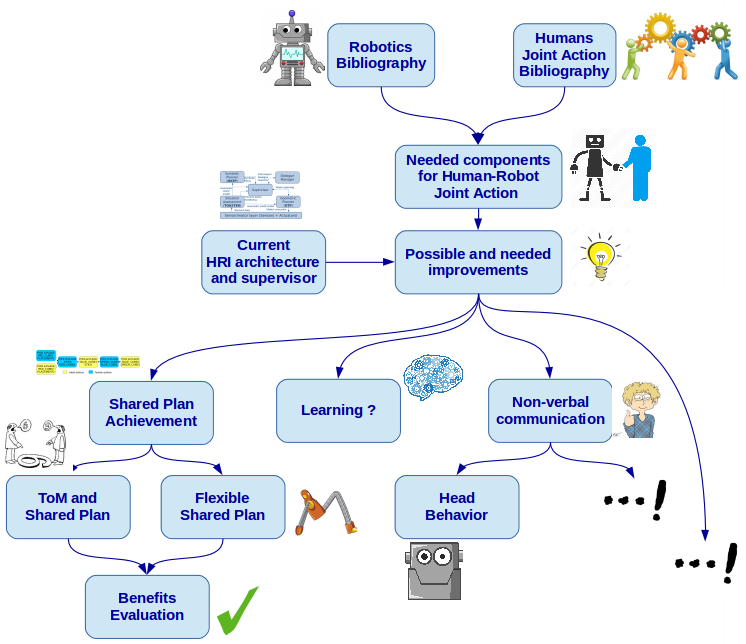
\includegraphics[width=\textwidth]{figs/Introduction/Plan.png}
    \caption{Organization of the contributions presented in the manuscript.}
    \label{fig:planIntro}
\end{figure}

One first subject where I saw possibilities of improvement was the way the robot elaborates and executes Shared Plans. This subject is treat in the second part of the manuscript and is decomposed in three chapters:
\begin{itemize}
\item First, I noticed that there was a gap between the perspective abilities of the robot and the Shared Plan execution. Indeed, several previous works endowed the robot with the ability to estimate how its human partners perceive the world and how to use this knowledge on several domains such as dialogue. However, there was no work to link this ability to the Shared Plan execution. In Chapter~\ref{ch:MS}, I will present how we endowed the robot with the ability to estimate the humans mental states, not only about the environment, but also concerning the state of the task and more particularly of the Shared Plan. Then, I will present how the robot is able to use these mental states to better communicate about divergent beliefs during Shared Plan execution.
\item Then, coming from discussions with psychologists on the subject, we noticed that the way the robot was dealing with Shared Plans was not "natural" for humans and not enough flexible. Indeed, in the previous system, the robot was taking all decisions during Shared Plan elaboration. It was choosing for each action who should perform it and with which specific objects. Imagine a table with several identical objects on it that the robot needs to clean in collaboration with a human. The robot would have decided at the beginning for each object who should take it and in which exact order. The human would have simply removed objects and adapts to the robot decisions. The Chapter~\ref{ch:SP} aims to reduce this gap. We first identified the needed decisions during Shared Plan elaboration and execution and we endowed the robot with the ability to decide which decisions should be taken at planning time and which one are better postponed at execution time. Then, we allowed the robot to take these decision by smoothly adapting to the human choices.
\item Finally, we wanted to evaluate the wholeness of the improvements bring to the Shared Plan achievement by the robot. We did it in Chapter~\ref{ch:Eval} both quantitatively in simulation and qualitatively with a user study in the real robot. These studies allowed to show the pertinence of the proposed ameliorations and to compare two different modes developed in the context of this work (in one mode the robot negotiates some needed decisions during Shared Plan execution while in the other the robot adapts to the human choices). Moreover, for the purpose of the user study, a questionnaire has been developed to evaluate the users feelings concerning the collaboration with the robot. This questionnaire has been validated (in term of inter coherence) thanks to the study data and is generic enough to be considered as a future tool for human-robot collaboration evaluation.
\end{itemize}

Then, I saw another interesting work subject concerning the non-verbal behavior of the robot. Indeed, during Joint Action between humans, Joint Action participants exchange a lot of information through non-verbal communication. It allows to increase fluency in the task execution and to align the knowledge of all participants. Consequently, for the robot to become a better Joint Action partner, it should be able to provide such information with its non-verbal behavior. In Chapter~\ref{ch:Acting}, we studied more especially the head behavior of the robot (there is plenty other ways to give information with non-verbal behavior, but it may more need a career than a thesis to study all of them). Based on the bibliography in social sciences and on previous works in robotics, we identified needed components of a robot head behavior adapted to the Joint Action. We studied more deeply some of them with an on-line video based study. To conclude this chapter, we present how these components can be implemented into a robot head behavior architecture.

Finally, in the context of the RoboErgoSum ANR project\footnote{http://roboergosum.isir.upmc.fr/}, I have been brought to work in collaboration with ISIR at Paris where researchers work a lot in learning for robot high level decision. In Chapter~\ref{ch:Learning}, with another PhD student of ISIR Erwan Renaudo, we studied how to combine planning and learning in the context of human-robot Joint Action. The idea is to take advantage from both sides in order to come up with decision level which is able to quickly learn how to smoothly adapt to the human choices during Joint Action execution.


\section*{Work environment}
\addcontentsline{toc}{section}{Work environment}

This thesis has been realized at LAAS-CNRS in the RIS team (Robotics and InteractionS). It was included in the general objective to build a robotics architecture for an autonomous robots which interacts with humans. 

\paragraph{Robot:} in all this thesis, for practical reasons, the developed algorithms have been implemented in a PR2 robot from Clearpath Robotics (previously Willow Garage)\footnote{http://wiki.ros.org/Robots/PR2}. However, these algorithms are generic enough to be implemented in other robots. The PR2 robot is a semi-humanoid robot which is able to navigate and manipulate objects (see Fig.\ref{fig:PR2}).

\begin{figure}[!h]
	\centering
    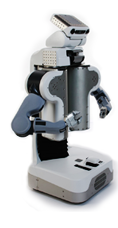
\includegraphics[width=0.25\textwidth]{figs/Introduction/PR2.png}
    \caption{The PR2 robot.}
    \label{fig:PR2}
\end{figure}

\paragraph{Humans and objects detection:} When interacting with humans during manipulation tasks, the robot needs to be able to localize and identify humans and objects. To avoid as much as possible perceptions issues which are not the focus of this thesis, the perception of humans and objects is simplified here. The humans are identified and perceived thanks to a motion capture system. They wear a helmet to get the position and orientation of their heads and a glove to get the position and orientation of their right hands (see Fig.~\ref{fig:Environment}). Concerning the objects, they are identified and localized with tags thanks to the robot cameras in its head.

\begin{figure}[!h]
	\centering
    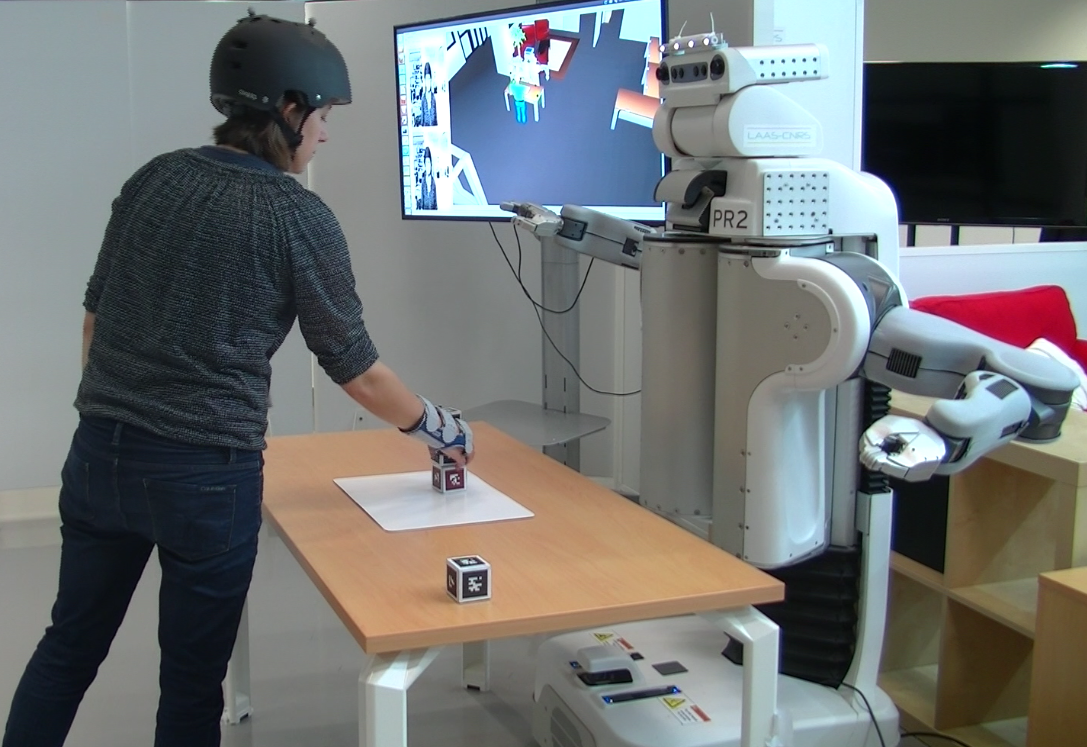
\includegraphics[width=0.7\textwidth]{figs/Introduction/SetUp.png}
    \caption{The PR2 robot interacting with a human to build a stack of cubes. The human is detected thanks to a motion capture system (helmet and glove) and the objects with tags.}
    \label{fig:Environment}
\end{figure}

\newpage
\section*{Publications}
\addcontentsline{toc}{section}{Publications}

The work presented in this thesis has led to several publications. They are listed here bellow (from the most recent to the oldest):
\begin{itemize}
\item \textbf{Devin, S.}, Clodic, A., Alami, R. (2017). About Decisions During Human-Robot Shared Plan Achievement: Who Should Act and How? The Ninth International Conference on Social Robotics. \textit{Submitted}.
\item \textbf{Devin, S.}, Alami, R. (2016). An implemented theory of mind to improve human-robot shared plans execution. In Human-Robot Interaction (HRI), 2016 11th ACM\/IEEE International Conference on (pp. 319-326). IEEE.
\item \textbf{Devin, S}., Milliez, G., Fiore, M., Clodic, A., Alami, R. (2016). Some essential skills and their combination in an architecture for a cognitive and interactive robot. Workshop In Human-Robot Interaction (HRI), 2016 11th ACM\/IEEE International Conference on (pp. 319-326). IEEE.
\item Khamassi, M., Girard, B., Clodic, A., \textbf{Sandra, D.}, Renaudo, E., Pacherie, E., Alami, R., Chatila, R. (2016). Integration of Action, Joint Action and Learning in Robot Cognitive Architectures. Intellectica (ARCo), 2016(65), 169-203.
\item Renaudo, E., \textbf{Devin, S.}, Girard, B., Chatila, R., Alami, R., Khamassi, M., Clodic, A. (2015). Learning to interact with humans using goal-directed and habitual behaviors. In RoMan 2015, Workshop on Learning for Human-Robot Collaboration.
\end{itemize}


\ifdefined\included
\else
\bibliographystyle{StyleThese}
\bibliography{These}
\end{document}
\fi

\setcounter{mtc}{1}

\part{From Human-Human Joint Action to a supervisor for Human-Robot Interaction}

\ifdefined\included
\else
\documentclass[english,a4paper,11pt,twoside]{StyleThese}
\usepackage{amsmath,amssymb}             % AMS Math
\usepackage[T1]{fontenc}
\usepackage[utf8x]{inputenc}
\usepackage{babel}
\usepackage{datetime}

\usepackage{lmodern}
\usepackage{tabularx}
%\usepackage{tabular}
\usepackage{multirow}

\usepackage{subfigure}
\usepackage{fancyvrb}
\usepackage{algorithmic}
\usepackage{algorithm}
\usepackage{mathtools}


\usepackage{hhline}
\usepackage[left=1.5in,right=1.3in,top=1.1in,bottom=1.1in,includefoot,includehead,headheight=13.6pt]{geometry}
\renewcommand{\baselinestretch}{1.05}

% Table of contents for each chapter

\usepackage[nottoc, notlof, notlot]{tocbibind}
\usepackage{minitoc}
\setcounter{minitocdepth}{2}
\mtcindent=15pt
% Use \minitoc where to put a table of contents

\usepackage{aecompl}


% Glossary / list of abbreviations

\usepackage[intoc]{nomencl}
\iftoggle{ThesisInEnglish}{%
\renewcommand{\nomname}{Glossary}
}{ %
\renewcommand{\nomname}{Liste des Abréviations}
}

\newcommand{\accom}[1]{\textcolor{red}{[#1]}}

\makenomenclature

% My pdf code

\usepackage{ifpdf}

\ifpdf
  \usepackage[pdftex]{graphicx}
  \DeclareGraphicsExtensions{.jpg}
  \usepackage[a4paper,pagebackref,hyperindex=true]{hyperref}
  \usepackage{tikz}
  \usetikzlibrary{arrows,shapes,calc}
\else
  \usepackage{graphicx}
  \DeclareGraphicsExtensions{.ps,.eps}
  \usepackage[a4paper,dvipdfm,pagebackref,hyperindex=true]{hyperref}
\fi

\graphicspath{{.}{images/}}

%% nicer backref links. NOTE: The flag ThesisInEnglish is used to define the
% language in the back references. Read more about it in These.tex

\iftoggle{ThesisInEnglish}{%
\renewcommand*{\backref}[1]{}
\renewcommand*{\backrefalt}[4]{%
\ifcase #1 %
(Not cited.)%
\or
(Cited in page~#2.)%
\else
(Cited in pages~#2.)%
\fi}
\renewcommand*{\backrefsep}{, }
\renewcommand*{\backreftwosep}{ and~}
\renewcommand*{\backreflastsep}{ and~}
}{%
\renewcommand*{\backref}[1]{}
\renewcommand*{\backrefalt}[4]{%
\ifcase #1 %
(Non cité.)%
\or
(Cité en page~#2.)%
\else
(Cité en pages~#2.)%
\fi}
\renewcommand*{\backrefsep}{, }
\renewcommand*{\backreftwosep}{ et~}
\renewcommand*{\backreflastsep}{ et~}
}

% Links in pdf
\usepackage{color}
\definecolor{linkcol}{rgb}{0,0,0.4} 
\definecolor{citecol}{rgb}{0.5,0,0} 
\definecolor{linkcol}{rgb}{0,0,0} 
\definecolor{citecol}{rgb}{0,0,0}
% Change this to change the informations included in the pdf file

\hypersetup
{
bookmarksopen=true,
pdftitle="Joint Action for Human-Robot Interaction",
pdfauthor="Sandra DEVIN", %auteur du document
pdfsubject="Thesis", %sujet du document
%pdftoolbar=false, %barre d'outils non visible
pdfmenubar=true, %barre de menu visible
pdfhighlight=/O, %effet d'un clic sur un lien hypertexte
colorlinks=true, %couleurs sur les liens hypertextes
pdfpagemode=None, %aucun mode de page
pdfpagelayout=SinglePage, %ouverture en simple page
pdffitwindow=true, %pages ouvertes entierement dans toute la fenetre
linkcolor=linkcol, %couleur des liens hypertextes internes
citecolor=citecol, %couleur des liens pour les citations
urlcolor=linkcol %couleur des liens pour les url
}

% definitions.
% -------------------

\setcounter{secnumdepth}{3}
\setcounter{tocdepth}{2}

% Some useful commands and shortcut for maths:  partial derivative and stuff

\newcommand{\pd}[2]{\frac{\partial #1}{\partial #2}}
\def\abs{\operatorname{abs}}
\def\argmax{\operatornamewithlimits{arg\,max}}
\def\argmin{\operatornamewithlimits{arg\,min}}
\def\diag{\operatorname{Diag}}
\newcommand{\eqRef}[1]{(\ref{#1})}

\usepackage{rotating}                    % Sideways of figures & tables
%\usepackage{bibunits}
%\usepackage[sectionbib]{chapterbib}          % Cross-reference package (Natural BiB)
%\usepackage{natbib}                  % Put References at the end of each chapter
                                         % Do not put 'sectionbib' option here.
                                         % Sectionbib option in 'natbib' will do.
\usepackage{fancyhdr}                    % Fancy Header and Footer

% \usepackage{txfonts}                     % Public Times New Roman text & math font
  
%%% Fancy Header %%%%%%%%%%%%%%%%%%%%%%%%%%%%%%%%%%%%%%%%%%%%%%%%%%%%%%%%%%%%%%%%%%
% Fancy Header Style Options

\pagestyle{fancy}                       % Sets fancy header and footer
\fancyfoot{}                            % Delete current footer settings

%\renewcommand{\chaptermark}[1]{         % Lower Case Chapter marker style
%  \markboth{\chaptername\ \thechapter.\ #1}}{}} %

%\renewcommand{\sectionmark}[1]{         % Lower case Section marker style
%  \markright{\thesection.\ #1}}         %

\fancyhead[LE,RO]{\bfseries\thepage}    % Page number (boldface) in left on even
% pages and right on odd pages
\fancyhead[RE]{\bfseries\nouppercase{\leftmark}}      % Chapter in the right on even pages
\fancyhead[LO]{\bfseries\nouppercase{\rightmark}}     % Section in the left on odd pages

\let\headruleORIG\headrule
\renewcommand{\headrule}{\color{black} \headruleORIG}
\renewcommand{\headrulewidth}{1.0pt}
\usepackage{colortbl}
\arrayrulecolor{black}

\fancypagestyle{plain}{
  \fancyhead{}
  \fancyfoot{}
  \renewcommand{\headrulewidth}{0pt}
}

%\usepackage{MyAlgorithm}
%\usepackage[noend]{MyAlgorithmic}
\usepackage[ED=MITT - STICIA, Ets=INP]{tlsflyleaf}
%%% Clear Header %%%%%%%%%%%%%%%%%%%%%%%%%%%%%%%%%%%%%%%%%%%%%%%%%%%%%%%%%%%%%%%%%%
% Clear Header Style on the Last Empty Odd pages
\makeatletter

\def\cleardoublepage{\clearpage\if@twoside \ifodd\c@page\else%
  \hbox{}%
  \thispagestyle{empty}%              % Empty header styles
  \newpage%
  \if@twocolumn\hbox{}\newpage\fi\fi\fi}

\makeatother
 
%%%%%%%%%%%%%%%%%%%%%%%%%%%%%%%%%%%%%%%%%%%%%%%%%%%%%%%%%%%%%%%%%%%%%%%%%%%%%%% 
% Prints your review date and 'Draft Version' (From Josullvn, CS, CMU)
\newcommand{\reviewtimetoday}[2]{\special{!userdict begin
    /bop-hook{gsave 20 710 translate 45 rotate 0.8 setgray
      /Times-Roman findfont 12 scalefont setfont 0 0   moveto (#1) show
      0 -12 moveto (#2) show grestore}def end}}
% You can turn on or off this option.
% \reviewtimetoday{\today}{Draft Version}
%%%%%%%%%%%%%%%%%%%%%%%%%%%%%%%%%%%%%%%%%%%%%%%%%%%%%%%%%%%%%%%%%%%%%%%%%%%%%%% 

\newenvironment{maxime}[1]
{
\vspace*{0cm}
\hfill
\begin{minipage}{0.5\textwidth}%
%\rule[0.5ex]{\textwidth}{0.1mm}\\%
\hrulefill $\:$ {\bf #1}\\
%\vspace*{-0.25cm}
\it 
}%
{%

\hrulefill
\vspace*{0.5cm}%
\end{minipage}
}

\let\minitocORIG\minitoc
\renewcommand{\minitoc}{\minitocORIG \vspace{1.5em}}

\usepackage{multirow}
%\usepackage{slashbox}

\newenvironment{bulletList}%
{ \begin{list}%
	{$\bullet$}%
	{\setlength{\labelwidth}{25pt}%
	 \setlength{\leftmargin}{30pt}%
	 \setlength{\itemsep}{\parsep}}}%
{ \end{list} }

\newtheorem{definition}{Définition}
\renewcommand{\epsilon}{\varepsilon}

% centered page environment

\newenvironment{vcenterpage}
{\newpage\vspace*{\fill}\thispagestyle{empty}\renewcommand{\headrulewidth}{0pt}}
{\vspace*{\fill}}

\usepackage{tablefootnote}

\sloppy
\begin{document}
\setcounter{chapter}{0} %% Numéro du chapitre précédent ;)
\dominitoc
\faketableofcontents
\fi

\chapter{From Human-Human Joint Action to Human-Robot Joint Action}
\minitoc

\section{Joint Action Theory}

A first step to endow robots with the ability to perform Joint Actions with humans is to understand how humans act together. As a working definition of Joint Action, we will use the one from \cite{sebanz2006joint}:

\begin{quote}
\textit{Joint action can be regarded as any form of social interaction whereby two or more individuals coordinate their actions in space and time to bring about a change in the environment.}
\end{quote}

A given number of prerequisites are needed for these individuals to achieve the so-called Joint Action. First of all, they need to agree on the change they want to bring in the environment, the conditions under which they will stay engaged in its realization and the way to do it. A number of works have studied this problematic, relative to \textit{commitment}, which I will develop in Sec.~\ref{subsec:commitment}. Then, as mentioned in the definition, the individuals need to coordinate their actions in space and time. This will be studied in Sec.~\ref{subsec:coordination}. Finally, in order to coordinate, each individual needs to be aware of the other, he needs to be able to perceive him and predict his actions. This part will be develop in Sec.~\ref{subsec:prediction}.

\subsection{Commitment}

\label{subsec:commitment}

The first prerequisite to achieve a Joint Action is to have a \textit{goal} to pursue and the \textit{intention} to achieve it. Let's define what is called a \textit{goal} and an \textit{intention} for a single person before going to a \textit{joint goal} and a \textit{joint intention}.

In \cite{tomasello2005understanding}, Tomasello et al. define what they call a \textit{goal} and an \textit{intention} and illustrate these definitions with an example and an associated figure (fig.~\ref{fig:intention}) where a person wants to open a box.

\begin{figure}[!h]
	\centering
    \includegraphics[width=0.8\textwidth]{figs/Chapter1/intention.png}
    \caption{Illustrative example of an intentional action by Tomasello et al. Here the human has for \textit{goal} for the box to be opened. He chooses a means to perform it and so forms an \textit{intention}.}
    \label{fig:intention}
\end{figure}
A \textit{goal} is defined here as the representation of the desired state by the agent (in the example, the goal is an open box) and, based on Bratman's work \cite{bratman1989intention}, an \textit{intention} is defined as an action plan the agent commits to in pursuit of a goal (in the example, the intention is to use a key to open the box). The \textit{intention} includes both a \textit{goal} and the means to achieve it.

In a same way, Cohen and Levesque propose in \cite{cohen1991teamwork} a formal definition of what they call a \textit{persistent goal}:

\begin{quote}
\textbf{Definition: } An agent has a \textit{persistent goal} relative to \textit{q} to achieve \textit{p} iff:
\begin{enumerate}
\item she believes that \textit{p} is currently false;
\item she wants \textit{p} to be true eventually;
\item it is true (and she knows it) that (2) will continue to hold until she comes to believe either that \textit{p} is true, or that it will neither be true, or that \textit{q} is false.
\end{enumerate}
\end{quote}

However, their definition of an \textit{intention} differs a little from the previous one. They define an \textit{intention} as a commitment to act in a certain mental state:

\begin{quote}
\textbf{Definition:} An agent \textit{intends} relative to some conditions to do an action just in case she has a persistent goal (relative to that condition) of having done the action, and, moreover, having done it, believing throughout that she is doing it.
\end{quote}

The \textit{intention} still includes the \textit{goal} but here it concerns more the fact that the agent commits to achieving the goal than the way to achieve it.

Let's now apply these principles to a Joint Action. One of the best known definition of \textit{joint intention} is the one of Bratman \cite{bratman1993shared}:
\begin{quote}
We intend to \textit{J} if and only if:
\begin{enumerate}
\item (a) I intend that we \textit{J} and (b) you intend that we \textit{J}.
\item I intend that we \textit{J} in accordance with and because of 1\textit{a}, 1\textit{b}, and meshing subplans of 1\textit{a} and 1\textit{b}; you intend that we \textit{J} in accordance with and because of 1\textit{a}, 1\textit{b}, and meshing subplans of 1\textit{a} and 1\textit{b}.
\item 1 and 2 are common knowledge between us.
\end{enumerate}
\end{quote}

This definition is taken back and illustrated by Tomasello et al. in \cite{tomasello2005understanding} where they reuse the example of the box to open (fig~\ref{fig:intention_jointe}).

\begin{figure}[!h]
	\centering
    \includegraphics[width=0.75\textwidth]{figs/Chapter1/intention_jointe.png}
    \caption{Illustrative example of a collaborative activity by Tomasello et al. Here the humans have for \textit{shared goal} to open the box together. They choose a means to perform it which takes into account the other capabilities and so form a \textit{joint intention}.}
    \label{fig:intention_jointe}
\end{figure}

The \textit{shared goal} is defined as the representation of a desired state plus the fact that it will be done in collaboration with other person(s) (in the example, they will open the box together) and a \textit{joint intention} is defined as a collaborative plan the agents commit to in order to achieve the \textit{shared goal} and which takes into account both agents individual plans (here an agent will hold the box with the clamp while the other open it with the cutter).

In a same way, Cohen and Levesque extend their definition of \textit{persistent goal} and \textit{intention} to a collaborative activity. They first define a \textit{weak achievement goal} as:
\begin{quote}
\textbf{Definition: } An agent has a \textit{weak achievement goal} relative to \textit{q} and with respect to a team to bring about \textit{p} if either of these conditions holds:
\begin{itemize}
\item The agent has a normal achievement goal to bring about \textit{p}, that is, the agent does not yet believe that \textit{p} is true and has \textit{p} eventually being true as goal.
\item The agent believes that \textit{p} is true, will never be true, or is irrelevant (that is, \textit{q} is false), \textit{but} has as a goal that the status of \textit{p} be mutually believed by all the team members.
\end{itemize}
\end{quote}

They then use this definition to define a \textit{joint persistent goal}:
\begin{quote}
\textbf{Definition: } A team of agents have a \textit{joint persistent goal} relative to \textit{q} to achieve \textit{p} just in case
\begin{itemize}
\item they mutually believe that \textit{p} is currently false;
\item they mutually know they all want \textit{p} to eventually be true;
\item it is true (and mutual knowledge) that until they come to mutually believe that \textit{p is true}, that \textit{p} will never be true, or that \textit{q} is false, they will continue to mutually believe that they each have \textit{p} as a weak achievement goal relative to \textit{q} and with respect to the team.
\end{itemize}
\end{quote}

They finally define a \textit{joint intention} as:
\begin{quote}
\textbf{Definition:} A team of agents \textit{jointly intends}, relative to some escape condition, to do an action iff the members have a joint persistent goal relative of that condition of their having done the action and, moreover, having done it mutually believing throughout that they were doing it.
\end{quote}

As previously, the definitions of Cohen and Levesque do no take into account the way to achieve the \textit{shared goal}, however, they introduce the interesting idea that agents are also engaged to communicate about the state of the \textit{shared goal}.

Concerning the way to achieve a \textit{shared goal}, mentioned into the definition of the \textit{joint intention} of Tomasello et al., Grosz and Sidner initially introduce and formalize the notion of \textit{Shared Plan} in \cite{grosz1988plans}, which is extended in \cite{grosz1999evolution}. The key properties of their model are as follows:
\begin{quote}
\begin{enumerate}
\item it uses individual intentions to establish commitment of collaborators to their joint activity
\item it establishes an agent's commitments to its collaborating partners' abilities to carry out their
individual actions that contribute to the joint activity
\item it accounts for helpful behavior in the context of collaborative activity
\item it covers contracting actions and distinguishes contracting from collaboration
\item the need for agents to communicate is derivative, not stipulated, and follows from the general
commitment to the group activity
\item the meshing of subplans is ensured it is also derivative from more general constraints.
\end{enumerate}
\end{quote}

With their definition, each agent does not necessarily know the whole \textit{Shared Plan} but only his own individual plan and the meshing subparts of the plan. The group has a \textit{Shared Plan}, but no individual member necessarily has the whole \textit{Shared Plan}.

In conclusion, the concepts concerning the commitment of agents to a collaborative activity that we will use in this thesis can be summarized as:
\begin{itemize}
\item A \textit{goal} will be represented as a desired state.
\item A\textit{shared goal} will be considered as a \textit{goal} to be achieved in collaboration with other partner(s). An agent is considered engaged in a \textit{shared goal} if he believes the goal is currently false, he wants the goal to be true and he will not give up on the goal unless he knows that the goal is achieved, not feasible or not relevant any more and he knows that his partners are aware of it.
\item A \textit{joint intention} will include a \textit{shared goal} and the way to realize it, represented as a \textit{Shared Plan} which will take into account the capacities of each agent and the potential conflicts between their actions. This \textit{Shared Plan} will not be necessarily completely known by all members of the group but all individuals will know their part of the plan and the meshing subparts.
\end{itemize}

If we apply this to the box example of Tomasello it gives us:
\begin{itemize}
\item "The box will be open" can be a \textit{goal} for an agent.
\item "The box will be open because we collaborate" can be a \textit{shared goal} for several agents. Once the agents agree to achieve this goal, they will not give up until the box is open (and the other agent knows it), the box can not be opened (and the other agent knows it) or there is no more need to open the box (and the other agent knows it).
\item A joint intention for two agents relative to the \textit{shared goal} to open the box will be, for example, that the first agent go get the opener, he gives it to the second agent and then the second agent opens the box with the opener. The sequence of action <go get the opener, give it, open the box> is the Shared Plan. The second agent does not need details concerning the part "go get the opener" while the first agent does not need details concerning the part "open the box".
\end{itemize}

\subsection{Perception and prediction}

\label{subsec:prediction}

One important thing for an agent when performing a Joint Action is to be able to perceive and predict the actions of his partner and their effects. Based on the works in \cite{sebanz2006joint}, \cite{pacherie2011phenomenology} and \cite{obhi2011moving} we identified several necessary abilities for this predictions:

\paragraph{Joint attention:} The capacity for an agent to share focus with his partner allows to share a representation of objects and events. It brings a better understanding of the other agent's knowledge and where his attention is focused and so, it helps the prediction of his possible next actions. Moreover, there should be a mutual manifestation of this joint attention, meaning that we should show that we share the other attention. 

\paragraph{Action observation:} Several studies have shown that when someone observes another person executing an action, a corresponding representation of the action is formed for the observer \cite{rizzolatti2004mirror}. This is done by what has been called the \textit{mirror-neuron} system. This behavior allows the observer to predict the outcomes of the actor's action. 

\paragraph{Co-representation:} An agent needs to have a representation of his partner, including his goal, his capacities and the social rules he is following. This representation also includes the knowledge of the partner on the Shared Plan, especially on the actions attributed to him. Having this representation will help to predict his future actions. For example, as a pedestrian knows that the car drivers follow the traffic regulations, he will be able to predict that they will stop if he sees a red traffic light.

\paragraph{Agency:} Sometimes, when there is a close link between an action performed by oneself and an action performed by someone else, it can be hard to distinguish who caused a particular effect. The capacity to attribute the effects to the right actor is called the sense of \textit{Agency}. This sense of \textit{Agency} is important in Joint Action in order to correctly predict the effects of each action.

\bigskip
Based on the same works as before and on \cite{sebanz2009prediction}, we can list several kinds of predictions to support Joint Action which can be done thanks to the abilities described previously :

\begin{itemize}
\item \textbf{What:} A first one is to predict what an agent will do. Two kinds of predictions, described in \cite{pacherie2011phenomenology}, can be distinguished here:
\begin{itemize}
\item \textit{action-to-goal:} this is supported by the \textit{mirror-neuron} system introduced before. Here the word goal designates the goal of an action, its purpose. The idea is that by observing an action, it is possible to predict its goal. For example, if we observe someone extending his arm toward an object we can predict that he will pick the object.
\item \textit{goal-to-action:} here the word goal designates the goal of a task, as defined in the previous subsection. Knowing this goal, it can be easy to predict which action an agent will perform.
\end{itemize}
\item \textbf{When:} another prediction which is necessary is the timing of an action. Knowing when an action will occur and how long it will take allows for a better coordination in time.
\item \textbf{Where:} a Joint Action usually takes place in a shared space. It is therefore necessary to predict the future position of the partner and his actions in order to coordinate in space.
\end{itemize} 


\subsection{Coordination}

\label{subsec:coordination}

The predictions discussed previously allow agents to coordinate during Joint Action. Two kinds of coordination are defined in \cite{knoblich20113} that both support Joint Action.

\paragraph{Emergent coordination:}
It is a coordinated behavior which occurs unintentionally, independently of any joint plan or common knowledge and due to perception-action couplings. Four types of sources of emergent coordination can be distinguished:
\begin{itemize}
\item \textit{Entrainment:} Entrainment is a process that leads to temporal coordination of two actors’ behavior, in particular, synchronization, even in the absence of a direct mechanical coupling. It is the case, for example, for two people seating in rocking chairs involuntary synchronizing their rocking frequencies \cite{richardson2007rocking}.
\item \textit{Affordances:} An object affordance represents the opportunities that an object provides to an agent for a certain action repertoire \cite{gibson1977perceiving}. For example, the different ways to grab a mug. Two kinds of affordances can lead to an emergent coordination: \textit{common affordances} and \textit{joint affordances}. When several agents have the same action repertoire and perceive the same object they have a \textit{common affordance}. This \textit{common affordance} can lead the agents to execute the same action. When an object has affordances for two or more peoples collectively, the agents have to synchronize for an action to occur. This is what is called \textit{joint affordances}. For example, a long two-handled saw affords cutting for two people acting together but not for either of them acting individually.
\item \textit{Perception-action matching:} As discussed before, observing an action activates corresponding representation in the observer's mind. This process can lead to involuntary mimicry of the observed action. Consequently, if two persons observe the same action, they can have the same reaction to mimic the action.
\item \textit{Action simulation:} The internal mechanisms activated during action observation not only allow to mimic the action but also to predict the effects of this action. If two people observe the same action and so predict the same effects, they can consequently have the same reaction. For example, two persons seeing the same object falling will have the same reaction to try to catch it.
\end{itemize}


\paragraph{Planned coordination:} 
While emergent coordination is unintentional, planned coordination requires for agents to plan their own actions in relation to Joint Action and others' actions.

One way for an agent to intentionally coordinate during Joint Action is to change his behavior compared to when he is acting alone. These changes of behavior are called \textit{coordination smoothers} in \cite{vesper2010minimal} and can be of several types:
\begin{itemize}
\item Making our behavior more predictable by doing for example wider or less variable movements
\item Structuring our own task in order to reduce the need of coordination. For example sharing the space or working turn by turn.
\item Producing coordination signals like looking someone who should act or counting down.
\item Changing the way we use an object by using an affordance more appropriate to a shared use.
\end{itemize}

Another way to coordinate is through communication. Indeed, Clark argues that two or more persons can not perform a Joint Action without communicating \cite{clark1996using}. Here the word communication includes both verbal and non-verbal communication. Clark also defines what he calls the \textit{common ground}: when two agents communicate, they necessarily have common knowledge and conventions. Moreover, when communicating, it is important to not only send a message but also to assure that the message has been understood as the sender intends it to be. This process to make the sender and the receiver mutually believe that the message has been understood well enough for current purposes is called \textit{grounding}.

In conclusion, in order to smoothly perform a Joint Action, an agent needs to:
\begin{itemize}
\item Developed sufficient perception and prediction abilities in order to coordinate in space and time. It needs to be done from basic motor commands to high level decisions.
\item Produce coordination signals understandable by his partners in order for them to predict the agent behavior.
\item Unsure that the signals he sends are well received by his partners.
\end{itemize}

\section{How to endow a robot with Joint Action abilities}

In this part we will do an overview of how the theory on human-human Joint Action can be applied to human-robot Joint Action. Following to what has been discussed on commitment, we will first see in Sec.~\ref{subsec:engagement} how the robot can engage in Joint Action and understand the intention of its human partners. Then, we will see in Sec.~\ref{subsec:perspective_taking} how the robot perceives the humans and can predict their actions by taking into account their perspectives and mental states. We will also see how the robot can coordinate during Joint Action in Sec.~\ref{subsec:coordination_robot}.

The parts which are linked to the work presented in this thesis will be more developed in the corresponding chapters.

\subsection{Engagement and Intention}

\label{subsec:engagement}

As for humans, robots need to be able to engage in Joint Action. A first prerequisite is to choose a goal to perform. This goal can be imposed by a direct order of the user, however, the robot also needs to be able to pro actively propose its help whenever a human needs it. To do so, the robot needs to be able to infer high-level goals by observing and reasoning on its human partners’ activities. This process is called plan recognition or, when a bigger focus is put on human-robot interaction aspects, intention recognition. Many works have been done concerning plan recognition using approaches such as classical planning \cite{ramirez2009plan}, probabilistic planning \cite{bui2003general} or logic-based techniques \cite{singla2011abductive}. Concerning intention recognition, works such as \cite{breazeal2009embodied} and \cite{baker2014modeling} take into account theory of mind aspects to deduce what the human is doing.

When direct orders have been received and humans intentions recognized, the robot needs to choose which goal to perform, also taking into account its own resources. This problem has not been addressed as a whole in the literature, however, some similar works can be seen as partial answers. For example, some deliberation systems allow to solve problems with multiple goals taking into account resources such as time \cite{georgeff1987reactive, ghallab1994representation, lemai2004interleaving} or energy level \cite{rabideau1999iterative}.

Once the robot is engaged in a Joint Action, it needs to be able to monitor other agents engagement. Indeed, it needs to understand if, for a reason, a human aborts the current goal and react accordingly. This can be done using gaze cues and gestures \cite{rich2010recognizing}, postures \cite{sanghvi2011automatic} but also context and humans mental states \cite{salam2015multi}.

Finally, once a goal is chosen, the robot needs to be able to establish a Shared Plan to achieve it with its human partners. Several works have been done in task planning to take into account the human \cite{cirillo2010human,Lallement2014hatp}. They allow the robot to reduce resource conflicts \cite{chakraborti2016planning}, take divergent beliefs into account \cite{guitton2012belief,talamadupula2014coordination} or promote stigmergic collaboration
for agents in co-habitation \cite{chakraborti2015planning}. 
Once the plan computed, the robot needs to be able to share/negotiate it with its partners. Several studies have been reported on how to communicate these plans. Some researchers studied how a system could acquire knowledge on plan decomposition from a user \cite{Mohseni2015} and how dialog can be used to teach new collaborative plans to the robot and to modify these plans \cite{petit2013coordinating}. In \cite{sorce2015proof}, the system is able to learn a plan from a user and transmit it to another user and in \cite{allen2002human} a computer agent is able to construct a plan in collaboration with a user. Finally, \cite{milliez2016using} presents a system where the robot shares the plan with a level of details which depends on the expertise of the user.

\subsection{Perspective taking and humans mental states}

\label{subsec:perspective_taking}

One of the first difference between a human and a robot is the way they perceive the world. To perceive its environment, the robot uses sensors to recognize and localize entities. These sensors return positions and orientations in the form of coordinates (\textit{x, y, z}, $\theta$, $\phi$, $\psi$). On the other hand, humans use relations between objects to describe their positions (e.g. the mug is on the kitchen table, oriented toward the window). To understand the human references and to
generate understandable utterances, the robot needs therefore
to build a semantic representation of the world, based on the
geometric data it collects from sensors. This process is called \textit{grounding} and has been developed in several works as \cite{mavridis2005grounded} or \cite{lemaignan2012grounding}.

However having its own semantic representation of the world is not enough for the robot, it also needs to take into account the point of view of its partners in order to better understand their goals and actions. To do so, the robot does what is called \textit{perspective taking}, it constructs a representation of the world from the humans perspectives \cite{breazeal2006using,milliez2014framework}. This ability can be used by the robot to choose its actions in order to influence others mental states \cite{gray2014manipulating}, solve ambiguous situations \cite{ros2010one} or to better interact during dialogue \cite{ferreira2015users}.

One important application of \textit{perspective taking} is human action recognition. Indeed, knowing what others are aware of is a first step to understand what they are doing. Then, the action recognition can be done based on Partially Observed Markov Decision Processes (POMDP) and Dynamic Bayesian Networks (DBN) \cite{baker2014modeling} or inverse reinforcement learning \cite{nagai2015probabilistic}.

This subject will be more developed and we will see, in Chapter \ref{ch:MS}, how we use \textit{perspective taking} to estimate mental states of the humans concerning the Shared Plan in order to improve their execution.


\subsection{Coordination}

\label{subsec:coordination_robot}

One of the most important and difficult challenges during human robot Joint Action is to coordinate. The problem appears at different levels during Joint Action. 

At a higher level, the humans and the robot need to coordinate their actions to fluidly execute the Shared Plan. The robot needs to execute its actions at the right time, monitor the ones of its partners and correctly communicate when needed. Several systems have been developed to do so, has \textit{Chaski} \cite{shah2011improved}, a task-level executor which uses insights from human-human teaming in order to minimize human idle time or \textit{Pike} an online executive that unifies intention recognition and plan adaptation to deal with temporal uncertainties during Shared Plan execution \cite{karpas2015robust}. A part of the work presented in the thesis is the extension of \textit{SHARY}, a supervisor allowing to execute Shared Plans into a complete human-aware architecture \cite{clodic2009shary}. We will notably see in Chapter \ref{ch:SP} how we extend it in order to execute flexible Shared Plans where part of the decisions are let to the execution.
 
One of the key aspects at this level of coordination is verbal and non-verbal communication. Concerning verbal communication, there are two ways to consider dialogue. The first one consists on seeing dialogue as a Joint Action. The second one is to see it as a tool for Joint Action. In practice, dialogue can be both, and, as developed in \cite{clark1996using}, there can be Joint Actions in Joint Actions. Several works in robotics developed modules allowing the robot to dialogue with humans in support to Joint Action \cite{roy2000spoken, lucignano2013dialogue, ferreira2015users}. To support dialogue and Joint Action in general, non verbal communication is very important. Its benefit has been shown for human-robot interaction \cite{breazeal2005effects} and ways to perform it have been studied, principally concerning gaze cues \cite{boucher2010facilitative, mutlu2009footing} but also postures \cite{hart2014gesture}. However, there is few works which study the use of non-verbal behavior during human-robot Joint Action where both partners are acting. This subject and the associated literature will be more developed in Chapter~\ref{ch:Acting}.

At a lower level, the robot needs to coordinate with its partners during action execution. To execute a task, the robot can be led to perform actions in collaboration with one or several humans. The principal action studied in HRI is handover, an action which seems simple as we do it in every day life but which, in fact, raises a number of challenges as, among others, approaching the other person \cite{walters2007robotic}, finding an acceptable posture to give the object \cite{cakmak2011human, mainprice2012sharing} or releasing the object with the good timing \cite{mason2005grip}. But, the robot also needs to coordinate when it is executing an action on its own. Indeed, it needs to share space and resources and its actions need to be understandable enough for its partners. To do so, the robot not only has to execute its actions in an efficient way, but also in a legible, acceptable and predictable way. This process can be compared to the \textit{coordination smoothers} described in \cite{vesper2010minimal} and one way to do it is through human-aware motion planing \cite{sisbot2012human, kruse2013human}.


\section{A three levels architecture}

We saw previously the different prerequisites to Joint Action, both between humans and in HRI. We will see now how the monitoring of Joint Action is organized around three different levels first with the theory of Pacherie concerning humans Joint Actions in Sec.~\ref{subsec:Pacherie} and then in the LAAS robotics architecture in Sec.~\ref{subsec:Archi}.

\subsection{The three levels of Pacherie}

\label{subsec:Pacherie}

As for the prerequisite of Joint Action, we will first introduce the concepts developed by Pacherie on Action and then, extend them to Joint Action. Pacherie argues in \cite{pacherie2008phenomenology} that intention in Action is composed of three levels which all have a specific role to play and which are organized as in fig.~\ref{fig:Pacherie}. 

\paragraph{Distal Intention:} 
This is the highest level of intention. In a first time, this level is in charge of forming an intention to act. It means that it is in charge of choosing a goal, a time to execute it and finding a plan to achieve it. Then, once the time comes to execute the plan, this level has to ensure its good execution. To do so, Pacherie takes back the definition of what is called \textit{rational guidance and control} \cite{buekens2001indexicaliteit}. This control takes two forms: 'tracking control' where we ensure that each successive step in the action plan is successfully implemented before moving to the next step and 'collateral control' where we control for the side effects of accomplishing an action.

\paragraph{Proximal Intention:}
This level inherits an action plan from the \textit{Distal Intention}. Its responsibility is, first, to anchor the received action plan which is defined in an abstract way in the situation of the action. It needs to integrate conceptual information
about the intended action inherited from the \textit{Distal Intention} with perceptual information about the current situation to yield a more definite representation of the action to be performed. Then, this level has to ensure that the imagined actions become current through situational control of their unfolding.

\paragraph{Motor Intention:}
This is the lowest level of intention. As for the other levels, it first has to make choices and then to monitor their executions. At this level, these choices concern motor commands, which are the physical ways to achieve the action inherited from the \textit{Proximal Intention}.


\begin{figure}[!h]
	\centering
    \includegraphics[width=0.8\textwidth]{figs/Chapter1/Pacherie.png}
    \caption{The intentional cascade by Pacherie. Distal, Proximal and Motor intentions coexist at the same time, each one controlling the action at a different level.}
    \label{fig:Pacherie}
\end{figure}

In \cite{pacherie2011phenomenology}, Pacherie extends these three levels to Joint Action. In the same way as before, these three new levels coexist at the same time, each one controlling the Joint Action at a different level.

\paragraph{Shared Distal Intention:}
Where \textit{Distal Intention} was responsible for intention, \textit{Shared Distal Intention} is responsible for joint intention. When performing a Joint Action, this level is the one responsible for the shared goal and the Shared Plan. As said in Sec.~\ref{subsec:commitment}, the agent does not have a whole representation of the Shared Plan here and part of his representation will be executed by someone else.

\paragraph{Shared Proximal Intention:}
This level has the same responsibilities as \textit{Proximal Intention}, however, the anchoring of the action plan needs to take care of the Joint Action partners and to be done in a coordinated way. During the monitoring part, the choices made previously need to be adapted to the others behavior.

\paragraph{Coupled Motor Intention:}
As for \textit{Motor Intention}, this level is responsible for the motor commands of the agent. During Joint Action, this level will be the one responsible for precise spatio-temporal coordination for the actions which need it (e.g. holding an object together).


\subsection{A three levels robotics architecture}

\label{subsec:Archi}

Ten years before Pacherie came with her action theory with three levels, the field of autonomous robotics was trying to build architectures and was already intuitively designing three similar levels. A first implemented architecture for autonomous robots is presented in \cite{alami1998architecture}, organized around these three levels (fig.~\ref{fig:FirstArchi}).

\begin{figure}[!h]
	\centering
    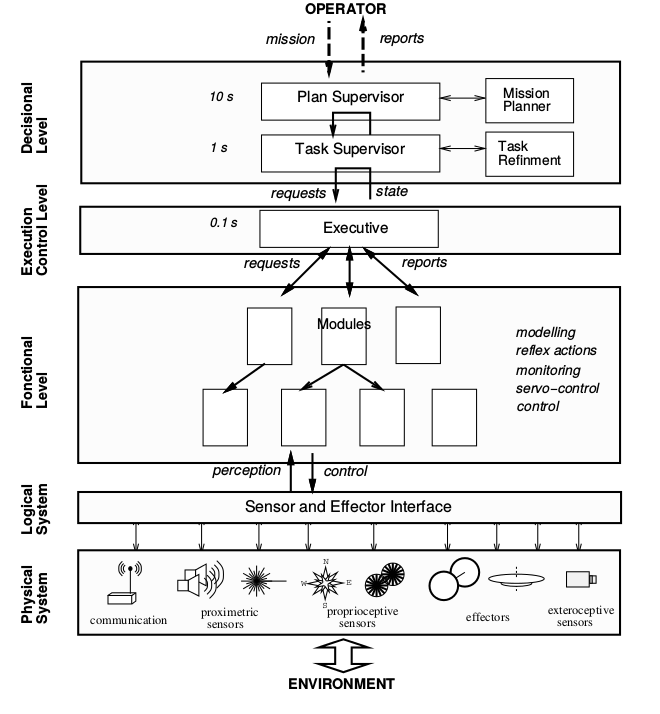
\includegraphics[width=0.8\textwidth]{figs/Chapter1/ArchitectureHold.png}
    \caption{One of the first architectures for autonomous robots. The architecture is divided in three main parts: decision, execution and functional levels.}
    \label{fig:FirstArchi}
\end{figure}

\paragraph{Decision level:}
This level can be compared to the \textit{Distal Intention} level of Pacherie. It is the one responsible for producing a task plan and supervising it. It sends actions to execute and receives reports from the \textit{execution level}.

\paragraph{Execution level:}
This level can be compared to the \textit{Proximal Intention} level of Pacherie. It receives from the \textit{decision level} the sequence of actions to be executed and selects, parametrizes and synchronizes dynamically the adequate functions of the \textit{functional level}.

\paragraph{Functional level:}
This level can be compared to the \textit{Motor Intention} level of Pacherie. It includes all the basic robot action and perception capacities (motion planning, vision, localization, tracking motion control...). 

\bigskip
In the past years, this architecture has been developed and adapted to the field of HRI. In recent works, we presented in \cite{devin2016some} a theoretical version of the architecture adapted to human-robot Joint Action and still based on the three levels of Pacherie (fig.~\ref{fig:ArchiThreeLevels}). The implemented version of this architecture will be presented in Chapter~\ref{ch:Sup}, where my contribution in the architecture will also be highlighted.

\begin{figure}[!h]
	\centering
    \includegraphics[width=\textwidth]{figs/Chapter1/architecture.png}
    \caption{Recent architecture for human-robot Joint Action. The architecture is organized in three levels corresponding to the ones defined by Pacherie.}
    \label{fig:ArchiThreeLevels}
\end{figure}

\paragraph{Distal level:}
As for \textit{Shared Distal Intention}, this level is responsible for goals and Shared Plans management. At this level, the robot is supposed to reason on its environment with high level representations. To do so, the robot is equipped with a \textbf{Situation Assessment} module which builds a symbolic representation of the robot environment. To be able to also reason about the humans knowledge, the robot is equipped with a \textbf{Mental State Management} module which constantly estimates humans mental states. With this information, the \textbf{Intention prediction} module is able to estimate humans intention and if the robot should propose its help or not. This module determines the goal of the robot and allows, during its execution, to monitor other agents engagement. Once the goal chosen, the \textbf{Shared Plan Elaboration} module allows the robot to construct and negotiate a Shared Plan to achieve the goal. Then, the \textbf{Shared Plan Achievement} module monitors the good execution of this Shared Plan. The last part of this level is the \textbf{Communication for Joint Action} module which allows the robot to verbally and non-verbally communicate during Joint Action. 

\paragraph{Proximal level:}
As for \textit{Shared Proximal Intention}, this level is in charge of anchoring the Shared Plan actions in the current situation. This level is composed of two parts: the \textbf{Actions Achievement} module which allows to call the adequate motor modules at the right time in order to perform robot actions and the \textbf{Human Actions Monitoring} module which allows to recognize and interpret humans actions with regard to the Shared Plan. These two modules communicate in order to coordinate robot actions to the humans ones.

\paragraph{Motor level:}
As for \textit{Coupled Motor Intention}, this level is in charge of motor commands of the robot. This level includes all modules allowing to control the robot actuators and interprets data from sensors. These modules, or at least a part of them, also take into account the humans as, for example, the human-aware geometric task and motion planner.

\subsection{Comparison to other robotics architectures}

We saw previously that human-robot interaction is a very complex field with many interesting subjects to study. As a consequence, few architectures allow the robot to execute tasks with humans in a fully autonomous way. 

In \cite{baxter2013cognitive}, Baxter et al. present a cognitive architecture built around DAIM (The Distributed Associative Interactive Memory), a memory component which allows the robot to classify the humans behavior. This architecture allows the robot to fluently align its behavior with the human while memorizing data on the interaction. However, several key aspects of human-robot Joint Action as human-aware action execution or theory of mind are missing in this architecture. 

Another cognitive architecture is presented in \cite{trafton2013act}. ACT-R/E, a cognitive architecture based on the ACT-R architecture, is used for human-robot interaction tasks. The architecture aims at simulating how humans think, perceive and act in the world. ACT-R/E has been tested in different scenarios, such as theory of mind and hide and seek, to show its capacity of modeling human behaviors and tought. This architecture has a big focus on the theory of mind and decisional aspects letting less space to the human-aware action execution or understanding, which are also big HRI challenges. 

\cite{beetz2010cram} proposes a cognitive architecture called CRAM (Cognitive Robot Abstract Machine) that integrates KnowRob \cite{tenorth2013knowrob}, a knowledge processing framework based on Prolog. CRAM is a very complete architecture dealing with problems such as manipulation, perception, plans or beliefs management. However, this architecture is more designed for a robot acting alone than a robot acting in collaboration with a human. Consequently, the architecture misses some key Joint Action aspects such as communication or humans actions monitoring.

An architecture based on inverse and forward models is presented in \cite{demiris2006hierarchical}. This architecture integrates interesting mechanisms which use human point of view to achieve learning. However, these aspects are limited to action recognition and execution and the architecture does not allow to deal with higher level decisional issues.

All of these architectures are really interesting and sharp in their respective predilection domains. However, even if our architecture may lack of some aspects as learning or memory management, its aim is to regroup a major part of the human-robot Joint Action aspects from higher level (intention management and decisional process) to lower level (human-aware execution, coordination and perception). Moreover, the architecture has been conceived in a modular enough way to allow the addition of new modules.

\ifdefined\included
\else
\bibliographystyle{StyleThese}
\bibliography{These}
\end{document}
\fi

\ifdefined\included
\else
\documentclass[english,a4paper,11pt,twoside]{StyleThese}
\usepackage{amsmath,amssymb}             % AMS Math
\usepackage[T1]{fontenc}
\usepackage[utf8x]{inputenc}
\usepackage{babel}
\usepackage{datetime}

\usepackage{lmodern}
\usepackage{tabularx}
%\usepackage{tabular}
\usepackage{multirow}

\usepackage{subfigure}
\usepackage{fancyvrb}
\usepackage{algorithmic}
\usepackage{algorithm}
\usepackage{mathtools}


\usepackage{hhline}
\usepackage[left=1.5in,right=1.3in,top=1.1in,bottom=1.1in,includefoot,includehead,headheight=13.6pt]{geometry}
\renewcommand{\baselinestretch}{1.05}

% Table of contents for each chapter

\usepackage[nottoc, notlof, notlot]{tocbibind}
\usepackage{minitoc}
\setcounter{minitocdepth}{2}
\mtcindent=15pt
% Use \minitoc where to put a table of contents

\usepackage{aecompl}


% Glossary / list of abbreviations

\usepackage[intoc]{nomencl}
\iftoggle{ThesisInEnglish}{%
\renewcommand{\nomname}{Glossary}
}{ %
\renewcommand{\nomname}{Liste des Abréviations}
}

\newcommand{\accom}[1]{\textcolor{red}{[#1]}}

\makenomenclature

% My pdf code

\usepackage{ifpdf}

\ifpdf
  \usepackage[pdftex]{graphicx}
  \DeclareGraphicsExtensions{.jpg}
  \usepackage[a4paper,pagebackref,hyperindex=true]{hyperref}
  \usepackage{tikz}
  \usetikzlibrary{arrows,shapes,calc}
\else
  \usepackage{graphicx}
  \DeclareGraphicsExtensions{.ps,.eps}
  \usepackage[a4paper,dvipdfm,pagebackref,hyperindex=true]{hyperref}
\fi

\graphicspath{{.}{images/}}

%% nicer backref links. NOTE: The flag ThesisInEnglish is used to define the
% language in the back references. Read more about it in These.tex

\iftoggle{ThesisInEnglish}{%
\renewcommand*{\backref}[1]{}
\renewcommand*{\backrefalt}[4]{%
\ifcase #1 %
(Not cited.)%
\or
(Cited in page~#2.)%
\else
(Cited in pages~#2.)%
\fi}
\renewcommand*{\backrefsep}{, }
\renewcommand*{\backreftwosep}{ and~}
\renewcommand*{\backreflastsep}{ and~}
}{%
\renewcommand*{\backref}[1]{}
\renewcommand*{\backrefalt}[4]{%
\ifcase #1 %
(Non cité.)%
\or
(Cité en page~#2.)%
\else
(Cité en pages~#2.)%
\fi}
\renewcommand*{\backrefsep}{, }
\renewcommand*{\backreftwosep}{ et~}
\renewcommand*{\backreflastsep}{ et~}
}

% Links in pdf
\usepackage{color}
\definecolor{linkcol}{rgb}{0,0,0.4} 
\definecolor{citecol}{rgb}{0.5,0,0} 
\definecolor{linkcol}{rgb}{0,0,0} 
\definecolor{citecol}{rgb}{0,0,0}
% Change this to change the informations included in the pdf file

\hypersetup
{
bookmarksopen=true,
pdftitle="Joint Action for Human-Robot Interaction",
pdfauthor="Sandra DEVIN", %auteur du document
pdfsubject="Thesis", %sujet du document
%pdftoolbar=false, %barre d'outils non visible
pdfmenubar=true, %barre de menu visible
pdfhighlight=/O, %effet d'un clic sur un lien hypertexte
colorlinks=true, %couleurs sur les liens hypertextes
pdfpagemode=None, %aucun mode de page
pdfpagelayout=SinglePage, %ouverture en simple page
pdffitwindow=true, %pages ouvertes entierement dans toute la fenetre
linkcolor=linkcol, %couleur des liens hypertextes internes
citecolor=citecol, %couleur des liens pour les citations
urlcolor=linkcol %couleur des liens pour les url
}

% definitions.
% -------------------

\setcounter{secnumdepth}{3}
\setcounter{tocdepth}{2}

% Some useful commands and shortcut for maths:  partial derivative and stuff

\newcommand{\pd}[2]{\frac{\partial #1}{\partial #2}}
\def\abs{\operatorname{abs}}
\def\argmax{\operatornamewithlimits{arg\,max}}
\def\argmin{\operatornamewithlimits{arg\,min}}
\def\diag{\operatorname{Diag}}
\newcommand{\eqRef}[1]{(\ref{#1})}

\usepackage{rotating}                    % Sideways of figures & tables
%\usepackage{bibunits}
%\usepackage[sectionbib]{chapterbib}          % Cross-reference package (Natural BiB)
%\usepackage{natbib}                  % Put References at the end of each chapter
                                         % Do not put 'sectionbib' option here.
                                         % Sectionbib option in 'natbib' will do.
\usepackage{fancyhdr}                    % Fancy Header and Footer

% \usepackage{txfonts}                     % Public Times New Roman text & math font
  
%%% Fancy Header %%%%%%%%%%%%%%%%%%%%%%%%%%%%%%%%%%%%%%%%%%%%%%%%%%%%%%%%%%%%%%%%%%
% Fancy Header Style Options

\pagestyle{fancy}                       % Sets fancy header and footer
\fancyfoot{}                            % Delete current footer settings

%\renewcommand{\chaptermark}[1]{         % Lower Case Chapter marker style
%  \markboth{\chaptername\ \thechapter.\ #1}}{}} %

%\renewcommand{\sectionmark}[1]{         % Lower case Section marker style
%  \markright{\thesection.\ #1}}         %

\fancyhead[LE,RO]{\bfseries\thepage}    % Page number (boldface) in left on even
% pages and right on odd pages
\fancyhead[RE]{\bfseries\nouppercase{\leftmark}}      % Chapter in the right on even pages
\fancyhead[LO]{\bfseries\nouppercase{\rightmark}}     % Section in the left on odd pages

\let\headruleORIG\headrule
\renewcommand{\headrule}{\color{black} \headruleORIG}
\renewcommand{\headrulewidth}{1.0pt}
\usepackage{colortbl}
\arrayrulecolor{black}

\fancypagestyle{plain}{
  \fancyhead{}
  \fancyfoot{}
  \renewcommand{\headrulewidth}{0pt}
}

%\usepackage{MyAlgorithm}
%\usepackage[noend]{MyAlgorithmic}
\usepackage[ED=MITT - STICIA, Ets=INP]{tlsflyleaf}
%%% Clear Header %%%%%%%%%%%%%%%%%%%%%%%%%%%%%%%%%%%%%%%%%%%%%%%%%%%%%%%%%%%%%%%%%%
% Clear Header Style on the Last Empty Odd pages
\makeatletter

\def\cleardoublepage{\clearpage\if@twoside \ifodd\c@page\else%
  \hbox{}%
  \thispagestyle{empty}%              % Empty header styles
  \newpage%
  \if@twocolumn\hbox{}\newpage\fi\fi\fi}

\makeatother
 
%%%%%%%%%%%%%%%%%%%%%%%%%%%%%%%%%%%%%%%%%%%%%%%%%%%%%%%%%%%%%%%%%%%%%%%%%%%%%%% 
% Prints your review date and 'Draft Version' (From Josullvn, CS, CMU)
\newcommand{\reviewtimetoday}[2]{\special{!userdict begin
    /bop-hook{gsave 20 710 translate 45 rotate 0.8 setgray
      /Times-Roman findfont 12 scalefont setfont 0 0   moveto (#1) show
      0 -12 moveto (#2) show grestore}def end}}
% You can turn on or off this option.
% \reviewtimetoday{\today}{Draft Version}
%%%%%%%%%%%%%%%%%%%%%%%%%%%%%%%%%%%%%%%%%%%%%%%%%%%%%%%%%%%%%%%%%%%%%%%%%%%%%%% 

\newenvironment{maxime}[1]
{
\vspace*{0cm}
\hfill
\begin{minipage}{0.5\textwidth}%
%\rule[0.5ex]{\textwidth}{0.1mm}\\%
\hrulefill $\:$ {\bf #1}\\
%\vspace*{-0.25cm}
\it 
}%
{%

\hrulefill
\vspace*{0.5cm}%
\end{minipage}
}

\let\minitocORIG\minitoc
\renewcommand{\minitoc}{\minitocORIG \vspace{1.5em}}

\usepackage{multirow}
%\usepackage{slashbox}

\newenvironment{bulletList}%
{ \begin{list}%
	{$\bullet$}%
	{\setlength{\labelwidth}{25pt}%
	 \setlength{\leftmargin}{30pt}%
	 \setlength{\itemsep}{\parsep}}}%
{ \end{list} }

\newtheorem{definition}{Définition}
\renewcommand{\epsilon}{\varepsilon}

% centered page environment

\newenvironment{vcenterpage}
{\newpage\vspace*{\fill}\thispagestyle{empty}\renewcommand{\headrulewidth}{0pt}}
{\vspace*{\fill}}

\usepackage{tablefootnote}

\sloppy
\begin{document}
\setcounter{chapter}{1} %% Numéro du chapitre précédent ;)
\dominitoc
\faketableofcontents
\fi

\chapter{Supervision for Human-Robot Interaction}
\minitoc

\label{ch:Sup}

\section{Role of the supervisor in the global architecture}

\label{sec:globalArchi}

One of the goals of my research group at LAAS-CNRS is to build a fully autonomous robot which interacts and performs Joint Actions with humans. To do so, an architecture for human-robot interaction has been developed and is constantly improved by the group. This architecture is composed of several modules and a simplified scheme of it can be found in Fig.~\ref{fig:GlobalArchi}.

\begin{figure}[!h]
	\centering
    \includegraphics[width=0.7\textwidth]{figs/Chapter2/archiGlobal.png}
    \caption{The global architecture for human-robot interaction implemented at LAAS-CNRS.}
    \label{fig:GlobalArchi}
\end{figure}

\paragraph{Sensorimotor layer:}
The lower level of the architecture is composed of modules which allow to communicate and control sensors and actuators. Among others, this layer is composed of modules interpreting sensors data to detect humans and objects and a module allowing to execute given trajectories by calling the adequate actuators.

\paragraph{Situation Assessment:}
The situation assessment is done by a software called TOASTER \cite{milliezThesis}. One of the functionalities of TOASTER is to build and maintain a consistent world state based on data coming from the sensorimotor layer. Geometric computations are done on this world state to compute symbolic predicates concerning the environment (e.g. \textit{<object, isOn, support>}, \textit{<object, isIn, box>}) and agents abilities and behaviors (e.g. \textit{<object, isVisibleBy, human>}, \textit{<object, isReachableBy, robot>}, \textit{human, isLookingToward, object}). TOASTER is also in charge of perspective taking: the previous predicates are constantly estimated and maintained not only from the robot’s point of view but also from the point of view of all humans concerned and perceived in the current context. All the data concerning the world state are stored and accessible through a temporal database.

\paragraph{Geometric Planner:}
In order to perform actions and movements adapted to the human proximity, our architecture is equipped with a geometric task and motion planner called GTP \cite{waldhart2016novel}. GTP allows to compute trajectories as well as objects placements and grasp. It does that at a level that is human understandable and readable by giving access to high level tasks such as Pick or Place while taking into account the human safety and comfort.

\paragraph{Symbolic Planner:}
For the robot to be able to synthesize Shared Plans, our architecture is equipped with HATP (Human-Aware Task Planner), a human-aware HTN (Hierarchical Task Network) task planner which allows the robot to compute and refine a plan both for itself and its humans partners, taking into account a number of social rules \cite{Lallement2014hatp}.
HATP has been specially designed to integrate a number of features that are meant to promote the synthesis of plans that are acceptable by humans and easily if not trivially understandable by them. It allows to specify the humans and robot capabilities in terms of actions they can execute. Several aspects such as human preferences and comfort, estimation of human effort to achieve a task in a given context and "social rules" are used in a cost-based approach to build "sufficiently good" human-robot Shared Plans.

\paragraph{Dialogue Manager:}
In order for the robot to communicate with humans, a basic dialogue manager has been integrated to the architecture. This module allows to give humans information concerning the environment (it verbalize predicates), ask basic questions (as asking if a human want to perform an action) and understand basic answers (mainly yes or no answers, the user can answer with buttons as there is no speech recognition in the system). 


\paragraph{Supervisor:}
The last module of the architecture is the supervisor. It is the one in charge of controlling collaborative activities. It chooses the robot goals and monitors the Shared Plan execution. To do so, it estimates humans mental states concerning the Shared Plan and takes them into account to decide when to perform actions or to communicate (verbally and/or non-verbally). It also interprets the information coming from the Situation Assessment module in order to recognize human actions like Pick or Place with regard to the Shared Plan. This module is an extension of \cite{clodic2009shary} and \cite{fiore2016planning} and is the major technical contribution of this thesis. Its internal architecture will be detailed in the next section.

\section{The supervisor architecture}

\begin{figure}[!h]
	\centering
    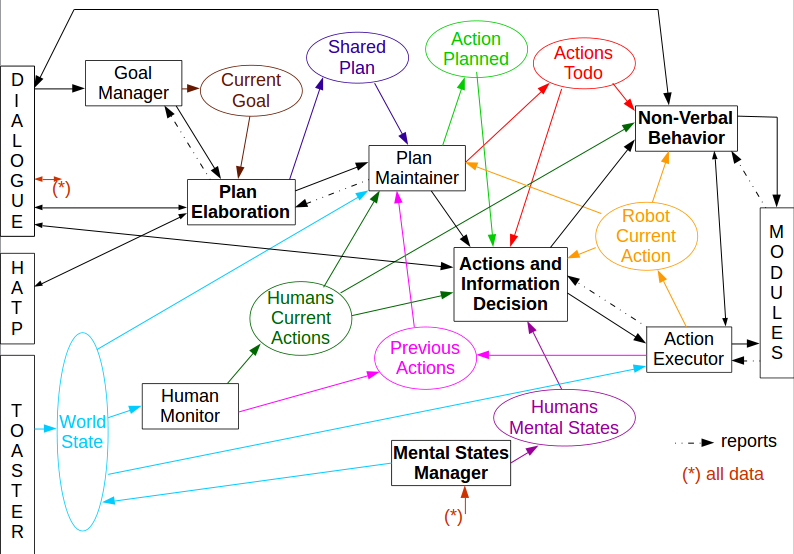
\includegraphics[width=\textwidth]{figs/Chapter2/ArchiSup.png}
    \caption{Architecture of the supervisor.}
    \label{fig:archiSup}
\end{figure}

The supervisor is composed of several modules and is fully implemented in ROS\footnote{http://www.ros.org/}. The complete scheme of its architecture can be found in Fig.~\ref{fig:archiSup}, however, as the figure is quite complex, each composing part of the supervisor will be represented and described individually in the next subsections. 

\subsection{Goal Manager}

The goal manager allows the robot to select and prioritize goals. It maintains a priority list of goals to perform. This list is updated with insert, abort or halt commands from dialogue or command line.

\begin{figure}[!h]
	\centering
    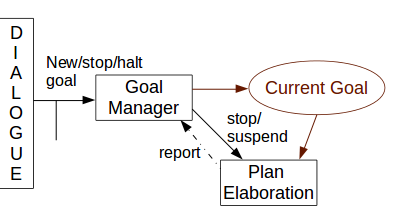
\includegraphics[width=0.5\textwidth]{figs/Chapter2/GoalManager.png}
    \caption{Interaction of the Goal Manager with the rest of the supervisor.}
    \label{fig:goalManager}
\end{figure}

The chosen goal is published in order for the Plan Elaboration module to find a Shared Plan to perform it. The module sends stop and suspend orders to the Plan Elaboration from which it receives reports concerning the success of the plan or the impossibility to find a plan.

This module is, for now, really basic. An interesting extension would be to integrate data coming from an intention recognition module concerning humans activities. This will allow the robot to choose if it should proactively offer its help based on this data and the goal orders it received. 

\subsection{Plan elaboration}

\begin{figure}[!h]
	\centering
    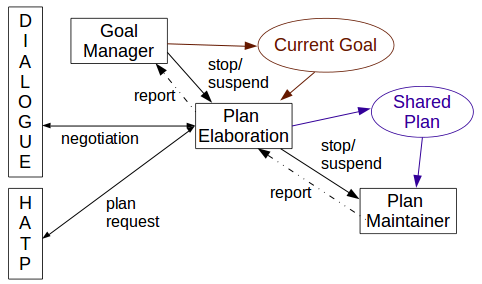
\includegraphics[width=0.6\textwidth]{figs/Chapter2/PlanElaboration.png}
    \caption{Interaction of the Plan Elaboration with the rest of the supervisor.}
    \label{fig:planElaboration}
\end{figure}

Once a goal received from the Goal Manager, the Plan Elaboration module is in charge of finding a Shared Plan to perform it. To do so, the module is able to call HATP (the Human Aware Task Planner described in Sec.~\ref{sec:globalArchi}) to compute a plan and the dialogue module to validate the plan or ask for missing information. One of the contributions of this thesis concerns the elaboration of more flexible Shared Plans where some decisions are left to the execution. This work is in part done in this module and will be developed in Chapter~\ref{ch:SP}.

The computed Shared Plan is then published in order for the Plan Maintainer module to deal with it. The stop and suspend orders received from the Goal Manager are transmitted to the Plan Maintainer module from which it receives reports concerning the success, failure or need of adaptation of the Shared Plan.

\subsection{Plan Maintainer}

The Plan Maintainer module is in charge of monitoring the execution of the Shared Plan based on the current world state and current and past actions. It publishes the list of actions from the Shared Plan which need to be performed at a given moment and the list of actions from the Shared Plan which need to be done later. It also checks the consistency of the plan and reports to the Plan Elaboration module in case of failure or unexpected situations.

\begin{figure}[!h]
	\centering
    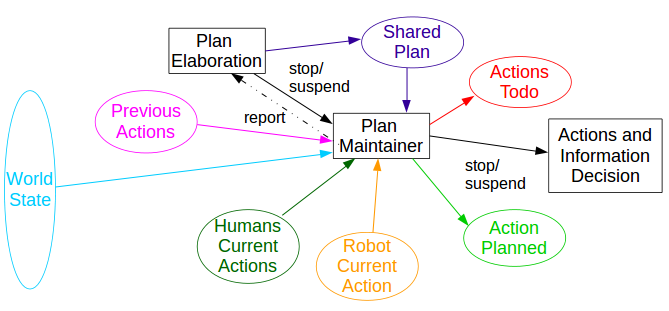
\includegraphics[width=0.8\textwidth]{figs/Chapter2/PlanMaintainer.png}
    \caption{Interaction of the Plan Maintainer with the rest of the supervisor.}
    \label{fig:planMaintainer}
\end{figure}

\subsection{Human Monitor}

The Human Monitor module allows to interpret the current world state which contains humans activity information in order to recognize basic humans actions like Pick or Place. This module is, for now, really basic as it is based mainly on distances between humans and objects. However, there is room for improvements by taking into account the context (e.g. the action the agent is supposed to perform) during action recognition or using probabilistic models.


\begin{figure}[!h]
	\centering
    \includegraphics[width=0.4\textwidth]{figs/Chapter2/HumanMonitor.png}
    \caption{Interaction of the Human Monitor with the rest of the supervisor.}
    \label{fig:humanMonitor}
\end{figure}

\subsection{Mental State Manager}

The Mental State Manager estimates the humans mental states concerning the current goal and Shared Plan. It bases its reasoning on all data published by the other supervisor modules and on the world states from all agents point of view given by TOASTER (see Sec.~\ref{sec:globalArchi}). This work is one of the thesis contribution and will be developed in Chapter \ref{ch:MS}. The composition of the estimated mental states will be given in Sec.~\ref{sec:data}. 

\begin{figure}[!h]
	\centering
    \includegraphics[width=0.5\textwidth]{figs/Chapter2/MSManager.png}
    \caption{Interaction of the Mental State Manager with the rest of the supervisor.}
    \label{fig:MSManager}
\end{figure}

\subsection{Robot Decision}

The Robot Decision module allows the robot to decide which action to execute and which information to give. Its decisions are based on the lists of current, planned and to execute actions as well as on the humans mental states. The way the robot uses these mental states to give pertinent information to humans is one of the thesis contribution and will be developed in Chapter \ref{ch:MS}. The decision of which action to execute has also been studied in this thesis and will be developed in Chapter \ref{ch:SP}.

\begin{figure}[h]
	\centering
    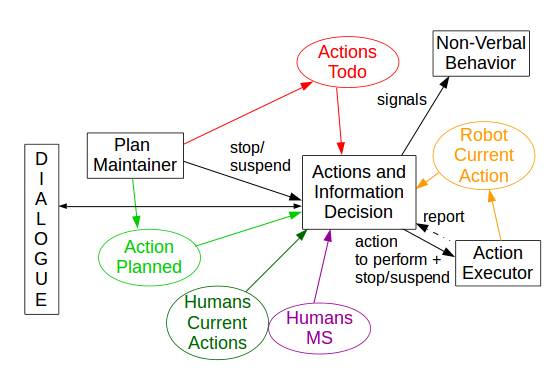
\includegraphics[width=0.7\textwidth]{figs/Chapter2/RobotDecision.png}
    \caption{Interaction of the Robot Decision module with the rest of the supervisor.}
    \label{fig:robotDecition}
\end{figure}

The Robot Decision module sends commands to the Action Executor from which it receives reports. It also communicates with the dialogue module and the Non-Verbal Behavior module to give the correct information.

\subsection{Action Executor}

The Action Executor is in charge of supervising robot actions. It receives actions to execute and stop or suspend orders from the robot decision and calls lower level modules to perform the given action in the best possible way. The action execution has been studied in this thesis and will be developed in Chapter \ref{ch:Acting}.

\begin{figure}[!h]
	\centering
    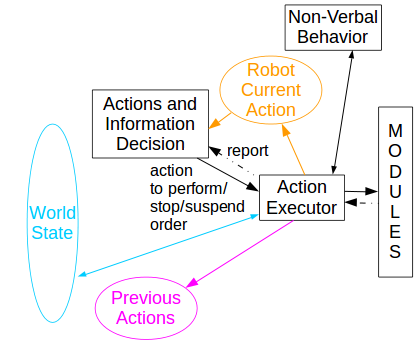
\includegraphics[width=0.5\textwidth]{figs/Chapter2/ActionExecutor.png}
    \caption{Interaction of the Action Executor with the rest of the supervisor.}
    \label{fig:actionExecutor}
\end{figure}

\newpage
\subsection{Non-Verbal Behavior}

This module allows to control the non-verbal behavior of the robot. In the current supervisor version, only the robot head behavior is concerned, but other type of non-verbal behaviors can be envisioned. The principles behind this module will be developed in Chapter \ref{ch:Acting}.

\begin{figure}[!h]
	\centering
    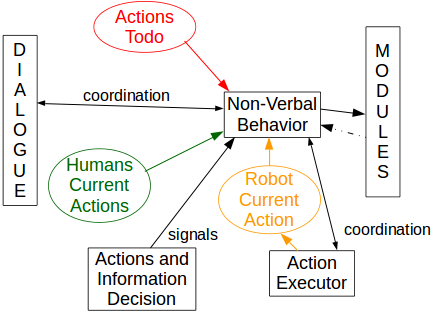
\includegraphics[width=0.5\textwidth]{figs/Chapter2/NVBehavior.png}
    \caption{Interaction of the Non-Verbal Behavior with the rest of the supervisor.}
    \label{fig:NVBehavior}
\end{figure}

The robot head behavior is based on the current robot action, the humans activities and the actions to perform. The module communicates with the dialogue module in order to coordinate and calls lower modules to control the robot. 

\section{Data representation}

\label{sec:data}

As seen in the previous section, several types of data are produced and used by the supervisor to take decisions. We will see now how we represent this data and this formalization will be used in the next chapters of the thesis.

The current state of the world from the robot point of view $WS$ is composed of a set of predicates $p$:
$$p = <entity, attribute, value>$$
For example, the fact that an object is on a table will be represented as $<object, isOn, table>$.

A goal $g$ is represented as:
$$g = <Name_g, Actors_g, Params_g, Obj_g>$$
where $Name_g$ allows to identify the goal, $Actors_g$ are the agents involved in the goal achievement, $Params_g$ are entities  (agents or objects) used to define precisely the goal and $Obj_g$ is a set of predicates representing the objective of the goal.
For example, if the robot has for goal to clean the table of the kitchen in collaboration with Bob by removing all items on it, this goal will be represented as:
$<Clean, <Robot, Bob>, <Kitchen\_table>, <<NULL, isOn, Kitchen\_table>>>$.
Finally, at its end, each goal $g$ is stored and associated with a label noted $label_g$ which can be equal either to DONE or ABORTED.

Then, a Shared Plan $SP$ is represented as:
$$SP = <id_p, A_p, L_p>$$
where $id_p$ is used to identify the plan, $A_p$ are the actions composing the plan and $L_p$ the links representing the order the actions should be executed (causal links).

A link $l \in L_p$ can be describe as:
 $$l = \langle prev_l, \ next_l \rangle$$
where $prev_l$ is the id of the action which needs to be achieved before the action with the id $next_l$ is performed. 

The actions composing the plan $A_p$ can be decomposed as:
$$A_p = <A_{prev}, A_{cur}, A_{next}, A_{later}>$$
where $A_{prev}$ are the actions of the plan already executed, $A_{cur}$ the actions currently executed, $A_{next}$ the actions which can be performed according to causal links and actions preconditions and $A_{later}$ the actions to be executed in the future.
Each of the set of actions previously introduced can be decomposed as:
$$<A = A^R, A^H, A^X>$$
where $A^R$ are the actions assigned to the robot, $A^H$ the actions assigned to the human and $A^X$ the actions not yet assigned. Indeed, we will see in Chapter~\ref{ch:SP} that not all actions are assigned to an actor during plan elaboration.
Finally, each action $a$ in $A_{prev}$ is associated with a label noted $label_a$ which can be equal either to DONE, FAILED or ABORTED.

An action $a$ can be represented as: 
$$a = < id_{a}, \ Name_{a}, \ Ag_{a}, \ Params_{a}, \ Precs_{a}, \ Effects_{a} >$$
Where $id_{a}$ is the action identifier and $Name_{a}$ represents its name. $Actors_{a}$ are the actors of the actions and $Params_{a}$ a set of parameters (objects or agents) which allows to define precisely the action. $Precs_{a}$ and $Effects_{a}$ are sets of predicates representing respectively the action preconditions and effects.
For example the action for the robot to place an object on a support will be defined as:$<0, place, Robot, <object, support>, <<object, isHoldBy, Robot>>, <<object, isOn, support>>>$.

The information concerning the state of the task is regrouped in what will be called the Task State $TS$:
$$TS = <g_R, SP, WS>$$
with $g_R$ the current goal of the robot, $SP$ the current Shared Plan and $WS$ the current world state from the robot point of view.

The robot also have a representation of humans mental state. The representation of the mental state $MS(H)$ of a human H is represented as:
$$MS(H) = <g_H, g_R(H), SP(H), WS(H)>$$
where $g_H$ is the goal the robot estimates the human is engaged in, $g_R(H)$ is the goal the robot estimates the human thinks the robot is performing, and $SP(H)$ and $WS(H)$ are the estimation of the Shared Plan and the World State from the human point of view.
$SP(H)$ is represented in the same way as the robot Shared Plan.


\ifdefined\included
\else
\bibliographystyle{StyleThese}
\bibliography{These}
\end{document}
\fi


\part{On the use of Shared Plans during Human-Robot Joint Action}

\ifdefined\included
\else
\documentclass[english,a4paper,11pt,twoside]{StyleThese}
\usepackage{amsmath,amssymb}             % AMS Math
\usepackage[T1]{fontenc}
\usepackage[utf8x]{inputenc}
\usepackage{babel}
\usepackage{datetime}

\usepackage{lmodern}
\usepackage{tabularx}
%\usepackage{tabular}
\usepackage{multirow}

\usepackage{subfigure}
\usepackage{fancyvrb}
\usepackage{algorithmic}
\usepackage{algorithm}
\usepackage{mathtools}


\usepackage{hhline}
\usepackage[left=1.5in,right=1.3in,top=1.1in,bottom=1.1in,includefoot,includehead,headheight=13.6pt]{geometry}
\renewcommand{\baselinestretch}{1.05}

% Table of contents for each chapter

\usepackage[nottoc, notlof, notlot]{tocbibind}
\usepackage{minitoc}
\setcounter{minitocdepth}{2}
\mtcindent=15pt
% Use \minitoc where to put a table of contents

\usepackage{aecompl}


% Glossary / list of abbreviations

\usepackage[intoc]{nomencl}
\iftoggle{ThesisInEnglish}{%
\renewcommand{\nomname}{Glossary}
}{ %
\renewcommand{\nomname}{Liste des Abréviations}
}

\newcommand{\accom}[1]{\textcolor{red}{[#1]}}

\makenomenclature

% My pdf code

\usepackage{ifpdf}

\ifpdf
  \usepackage[pdftex]{graphicx}
  \DeclareGraphicsExtensions{.jpg}
  \usepackage[a4paper,pagebackref,hyperindex=true]{hyperref}
  \usepackage{tikz}
  \usetikzlibrary{arrows,shapes,calc}
\else
  \usepackage{graphicx}
  \DeclareGraphicsExtensions{.ps,.eps}
  \usepackage[a4paper,dvipdfm,pagebackref,hyperindex=true]{hyperref}
\fi

\graphicspath{{.}{images/}}

%% nicer backref links. NOTE: The flag ThesisInEnglish is used to define the
% language in the back references. Read more about it in These.tex

\iftoggle{ThesisInEnglish}{%
\renewcommand*{\backref}[1]{}
\renewcommand*{\backrefalt}[4]{%
\ifcase #1 %
(Not cited.)%
\or
(Cited in page~#2.)%
\else
(Cited in pages~#2.)%
\fi}
\renewcommand*{\backrefsep}{, }
\renewcommand*{\backreftwosep}{ and~}
\renewcommand*{\backreflastsep}{ and~}
}{%
\renewcommand*{\backref}[1]{}
\renewcommand*{\backrefalt}[4]{%
\ifcase #1 %
(Non cité.)%
\or
(Cité en page~#2.)%
\else
(Cité en pages~#2.)%
\fi}
\renewcommand*{\backrefsep}{, }
\renewcommand*{\backreftwosep}{ et~}
\renewcommand*{\backreflastsep}{ et~}
}

% Links in pdf
\usepackage{color}
\definecolor{linkcol}{rgb}{0,0,0.4} 
\definecolor{citecol}{rgb}{0.5,0,0} 
\definecolor{linkcol}{rgb}{0,0,0} 
\definecolor{citecol}{rgb}{0,0,0}
% Change this to change the informations included in the pdf file

\hypersetup
{
bookmarksopen=true,
pdftitle="Joint Action for Human-Robot Interaction",
pdfauthor="Sandra DEVIN", %auteur du document
pdfsubject="Thesis", %sujet du document
%pdftoolbar=false, %barre d'outils non visible
pdfmenubar=true, %barre de menu visible
pdfhighlight=/O, %effet d'un clic sur un lien hypertexte
colorlinks=true, %couleurs sur les liens hypertextes
pdfpagemode=None, %aucun mode de page
pdfpagelayout=SinglePage, %ouverture en simple page
pdffitwindow=true, %pages ouvertes entierement dans toute la fenetre
linkcolor=linkcol, %couleur des liens hypertextes internes
citecolor=citecol, %couleur des liens pour les citations
urlcolor=linkcol %couleur des liens pour les url
}

% definitions.
% -------------------

\setcounter{secnumdepth}{3}
\setcounter{tocdepth}{2}

% Some useful commands and shortcut for maths:  partial derivative and stuff

\newcommand{\pd}[2]{\frac{\partial #1}{\partial #2}}
\def\abs{\operatorname{abs}}
\def\argmax{\operatornamewithlimits{arg\,max}}
\def\argmin{\operatornamewithlimits{arg\,min}}
\def\diag{\operatorname{Diag}}
\newcommand{\eqRef}[1]{(\ref{#1})}

\usepackage{rotating}                    % Sideways of figures & tables
%\usepackage{bibunits}
%\usepackage[sectionbib]{chapterbib}          % Cross-reference package (Natural BiB)
%\usepackage{natbib}                  % Put References at the end of each chapter
                                         % Do not put 'sectionbib' option here.
                                         % Sectionbib option in 'natbib' will do.
\usepackage{fancyhdr}                    % Fancy Header and Footer

% \usepackage{txfonts}                     % Public Times New Roman text & math font
  
%%% Fancy Header %%%%%%%%%%%%%%%%%%%%%%%%%%%%%%%%%%%%%%%%%%%%%%%%%%%%%%%%%%%%%%%%%%
% Fancy Header Style Options

\pagestyle{fancy}                       % Sets fancy header and footer
\fancyfoot{}                            % Delete current footer settings

%\renewcommand{\chaptermark}[1]{         % Lower Case Chapter marker style
%  \markboth{\chaptername\ \thechapter.\ #1}}{}} %

%\renewcommand{\sectionmark}[1]{         % Lower case Section marker style
%  \markright{\thesection.\ #1}}         %

\fancyhead[LE,RO]{\bfseries\thepage}    % Page number (boldface) in left on even
% pages and right on odd pages
\fancyhead[RE]{\bfseries\nouppercase{\leftmark}}      % Chapter in the right on even pages
\fancyhead[LO]{\bfseries\nouppercase{\rightmark}}     % Section in the left on odd pages

\let\headruleORIG\headrule
\renewcommand{\headrule}{\color{black} \headruleORIG}
\renewcommand{\headrulewidth}{1.0pt}
\usepackage{colortbl}
\arrayrulecolor{black}

\fancypagestyle{plain}{
  \fancyhead{}
  \fancyfoot{}
  \renewcommand{\headrulewidth}{0pt}
}

%\usepackage{MyAlgorithm}
%\usepackage[noend]{MyAlgorithmic}
\usepackage[ED=MITT - STICIA, Ets=INP]{tlsflyleaf}
%%% Clear Header %%%%%%%%%%%%%%%%%%%%%%%%%%%%%%%%%%%%%%%%%%%%%%%%%%%%%%%%%%%%%%%%%%
% Clear Header Style on the Last Empty Odd pages
\makeatletter

\def\cleardoublepage{\clearpage\if@twoside \ifodd\c@page\else%
  \hbox{}%
  \thispagestyle{empty}%              % Empty header styles
  \newpage%
  \if@twocolumn\hbox{}\newpage\fi\fi\fi}

\makeatother
 
%%%%%%%%%%%%%%%%%%%%%%%%%%%%%%%%%%%%%%%%%%%%%%%%%%%%%%%%%%%%%%%%%%%%%%%%%%%%%%% 
% Prints your review date and 'Draft Version' (From Josullvn, CS, CMU)
\newcommand{\reviewtimetoday}[2]{\special{!userdict begin
    /bop-hook{gsave 20 710 translate 45 rotate 0.8 setgray
      /Times-Roman findfont 12 scalefont setfont 0 0   moveto (#1) show
      0 -12 moveto (#2) show grestore}def end}}
% You can turn on or off this option.
% \reviewtimetoday{\today}{Draft Version}
%%%%%%%%%%%%%%%%%%%%%%%%%%%%%%%%%%%%%%%%%%%%%%%%%%%%%%%%%%%%%%%%%%%%%%%%%%%%%%% 

\newenvironment{maxime}[1]
{
\vspace*{0cm}
\hfill
\begin{minipage}{0.5\textwidth}%
%\rule[0.5ex]{\textwidth}{0.1mm}\\%
\hrulefill $\:$ {\bf #1}\\
%\vspace*{-0.25cm}
\it 
}%
{%

\hrulefill
\vspace*{0.5cm}%
\end{minipage}
}

\let\minitocORIG\minitoc
\renewcommand{\minitoc}{\minitocORIG \vspace{1.5em}}

\usepackage{multirow}
%\usepackage{slashbox}

\newenvironment{bulletList}%
{ \begin{list}%
	{$\bullet$}%
	{\setlength{\labelwidth}{25pt}%
	 \setlength{\leftmargin}{30pt}%
	 \setlength{\itemsep}{\parsep}}}%
{ \end{list} }

\newtheorem{definition}{Définition}
\renewcommand{\epsilon}{\varepsilon}

% centered page environment

\newenvironment{vcenterpage}
{\newpage\vspace*{\fill}\thispagestyle{empty}\renewcommand{\headrulewidth}{0pt}}
{\vspace*{\fill}}

\usepackage{tablefootnote}

\sloppy
\begin{document}
\setcounter{chapter}{2} %% Numéro du chapitre précédent ;)
\dominitoc
\faketableofcontents
\fi

\chapter{Taking Humans Mental States into account while executing Shared Plans}
\minitoc

\label{ch:MS}

\section{Motivations}

When collaborating with humans, it is primordial for the robot to not consider humans as obstacles or tools impacting the environment. As humans are social creatures, the robot must take into account their comfort and so, their point of view. Several works already allow robots to estimate humans perspective and beliefs concerning their environment. In order to improve human-robot Joint Action, the robot must be able to take this information into account when taking decision on how to act or what to communicate. Even if several works have been done on how to integrate humans perspective in dialogue or use it to help the understanding of humans behavior, there is still a gap when it comes to use it during Shared Plan execution. This work aims to start filling this gap by extending the robot knowledge on humans mental states to the joint task and using it to better communicate during Shared Plan execution. It has been the subject of a publication into the HRI conference \cite{devin2016implemented}.

\section{Theory of Mind}

\subsection{Social Sciences literature}

Theory of the Mind (ToM) refers to the ability humans have to recognize and attribute mental states not only to themselves but to other people, to understand that feelings and beliefs we have may be different than the one of the others and to take others mental states into account when taking decisions. ToM has been deeply studied in psychology, notably in the developmental domain \cite{baron1985does, premack1978does}. \cite{verbrugge2008learning} defines what is called "order" of ToM:
\begin{quote}
"To have a first-order ToM is to assume that someone’s beliefs,
thoughts and desires influence one’s behavior. A first-order thought could be: ‘He does not know that his book is on the table’. In second-order ToM it is also recognized that to predict others’ behavior, the desires and beliefs that they have of one’s self and the predictions of oneself by others must be taken into account. So, for example, you can realize that what someone expects you to do will affect his behavior. For example, ‘(I know) he does not know that I know his book is on the table’ would be part of my second-order ToM. To have a third-order ToM is to assume others to have a second-order ToM, etc."
\end{quote}
There is an infinite number of orders, however, studies have shown that orders above the second one do not help in cooperative tasks \cite{de2014theory} and those above the third one do not help for competitive games \cite{de2014theory}.


\begin{figure*}[!h]
    \centering
    \subfigure[Perceptual perspective taking: two individuals can have a different representation of their environment considering their locations.]{
        \centering
        \includegraphics[width=0.4\textwidth]{figs/Chapter3/perceptual.jpg}
       \label{subfig:perceptual}
   }
    %~
    \subfigure[Conceptual perspective taking: here Bob attributes to Alice a belief concerning the box. He thinks Alice thinks the box is empty.]{
        \centering
        \includegraphics[width=0.4\textwidth]{figs/Chapter3/conceptual.jpg}
       \label{subfig:conceptual}
    }
    \caption{Illustration of perceptual and conceptual perspective taking.}
\end{figure*}

ToM includes the notion of perspective taking: the capacity for a person to reason by taking the point of view of someone else. Studied in literature \cite{tversky1999speakers, flavell1992perspectives}, perspective taking is crucial during humans interaction and studies have demonstrated that individuals who lack of this ability have difficulties in their daily social interactions \cite{frick2014picturing}. Two levels of perspective taking are defined in \cite{flavell1977development}: perceptual and conceptual perspective taking. Perceptual perspective taking refers to the capacity of a person to understand that others have a different perception of the world (fig~\ref{subfig:perceptual}). Conceptual perspective taking refers to the capacity of a person to attribute beliefs and feelings to others (fig~\ref{subfig:conceptual}).

\begin{figure}[!h]
	\centering
    \includegraphics[width=0.7\textwidth]{figs/Chapter3/sally.jpg}
    \caption{The Sally and Anne test: it allows to check the capacity of someone to attribute a false-belief to another person. Illustration from the work of Axel Scheffler.}
    \label{fig:sally}
\end{figure}

To check if an individual has ToM capacities, several tests have been developed in psychology. One of the most famous is the Sally and Anne test (fin~\ref{fig:sally}). This test allows to check the capacity of someone to attribute a false-belief to another person and have been reused in robotics to validate robots perspective taking abilities \cite{hiatt2010cognitive, milliez2014framework}.

\subsection{Robotics background}

One of the pioneer work in robotics Theory of Mind is \cite{scassellati2002theory}. Scassellati presents two models from social sciences (Leslie \cite{leslie1984spatiotemporal} et Baron-Cohen \cite{baron1997mindblindness}) and proposes a model on how to implement ToM in robotics. However, the implementation of this model did not go further than perception level.

Then, several works have been done in order to endow robots with perspective taking abilities. Using ACT-R architecture \cite{anderson2004integrated}, the team of Hiatt and Trafton models mechanisms used during the Sally and Anne test and constructs a model that learns to deal with false belief in order to pass this test \cite{hiatt2010cognitive}. They extend this work to second-order in \cite{hiatt2015understanding} and to spatial reasoning in \cite{hiatt2004cognitive}. The Sally and Anne test has also been passed in \cite{milliez2014framework} where the robot constructs a semantic representation of the world from its partners point of view. In \cite{berlin2006perspective}, authors present a way to record different beliefs of other agents and so to have a memory of perspective taking. Finally, \cite{johnson2005perspective} presents a system which computes perspective taking based on forward and inverse visual models.

Perspective taking abilities have been used in robotics for several purposes. It has been used in \cite{hiatt2011accommodating} to deal with uncertainty in humans behavior and in \cite{ros2010solving} to solve ambiguous references to an object. One important application of perspective taking is action recognition. \cite{johnson2005perceptual} takes the visual point of view of humans to improve action recognition, Dynamic Bayesian Networks (DBN) are used in \cite{baker2014modeling} or inverse reinforcement learning  in \cite{nagai2015probabilistic}. The human perspective is also used in \cite{breazeal2006using} to learn a task from a situation that can be ambiguous from the robot point of view and in \cite{gray2014manipulating} to choose actions with the adequate effects in order to manipulate humans mental models. Finally, \cite{gorur2017toward} uses perspective taking to infer humans intention and adapt robot decision.

Concerning Shared Plans, perspective taking can be used to help their elaboration in order to add communication actions to solve divergent beliefs \cite{guitton2012belief}. Then, the human perspective is used to share the plan with a level of details depending of human knowledge \cite{milliez2016using}. However, there is no previous work concerning the management of Shared Plans execution taking into account the human point of view. 

\section{Assumptions}


The work presented in this chapter concerns the estimation of humans knowledge on the task and its use to help the Shared Plan execution. To do so, we make several assumptions:

\paragraph{Commitment:} we do not focus in this works on issues related to commitment. Consequently, we consider here that the joint goal has already been established. We also consider that none of the humans will abort the goal unless he knows that the goal is not achievable any more.

\paragraph{Shared Plan:} the focus of this work concerns rather the Shared Plan execution than the Shared Plan elaboration. In the examples presented in Sec.~\ref{sec:resultsTOM}, the Shared Plan is computed by the robot, however, the processes presented in this chapter hold regardless of the way the robot gets the Shared Plan (e.g. it can be imposed by a human or negotiated through dialogue). This chapter will treat only the issues related to ToM usage in Shared Plan execution, the other aspects of Shared Plan management will be more developed in Chapter \ref{ch:SP}.

\paragraph{ToM order:} this work implements a first-order ToM for the robot (i.e. the robot has knowledge about the human knowledge on the task), the higher orders are not managed for now. It means that the robot has its knowledge concerning the task (0-order) and the knowledge of the human concerning the task (1st order) but does not have knowledge concerning what the human knows about what the robot knows about the task (2nd order).

\paragraph{Humans perception:} we make the assumption here that a human will see and understand an action of another agent (mainly robot actions) when he is present and looking at the agent. We
also assume that when he is present, the human is able to hear and understand the information verbalized by the robot.

\paragraph{Robot capacities:} we consider that the robot is able to perform simple high level actions like Pick, Place or Drop. We also assume that the robot is able to ask to a human to perform an action and to inform him about the state of the environment, the goal or an action. The robot is able to detect and localize objects and agents
and to recognize simple high level actions performed by a human like Pick, Place or Drop. Let us also note that the ways the robot achieves actions (e.g. human-aware motion planning and execution) and recognizes humans’ actions are outside of the scope of this chapter.

\paragraph{Communication:} this work consists mainly in finding which information to give to the human and when. We do not focus here on how we give this information (here we use the basic dialogue module described in Chapter~\ref{ch:Sup} but more complex communication mechanisms can be envisioned). 

\section{Estimating Humans Mental States}

As stated previously, the goal of this work is to fill the gap between existing perspective taking abilities of the robot and Shared Plan execution. A first step to do so is to extend the knowledge of the robot concerning humans mental states to information concerning the Shared Plan. As saw in Chapter~\ref{ch:Sup}, the mental state of a human H will be described as:
$$MS(H) = <g_H, g_R(H), SP(H), WS(H)>$$
where $g_H$ is the goal the robot estimates the human is engaged in, $g_R(H)$ is the goal the robot estimates the human thinks the robot is performing, and $SP(H)$ and $WS(H)$ are the estimation of the Shared Plan and the World State from the human point of view. 

The process to estimate the humans mental states will be noted in the following of the thesis as the operator:
$$MS(H) \leftarrow ESTIMATE\_MS(MS(H), TS)$$

with $TS$ the state of the task from the robot point of view as stated in Chapter~\ref{ch:Sup}.
We will see now how we estimates each of the mental states components. The terms used in the following algorithms and formulas are reminded in Appendix \ref{chap:annexe1}.

\subsection{Goal management ($g_H$ and $g_R(H)$ computation)}

As stated previously, we do not focus in this work on issues related to goal management. Consequently, the computation of humans mental states concerning goals remains basic. However, a more complex one can be envisioned, for example using intention recognition, with the same representation. As a reminder, a goal is defined as:
$$g = <Name_g, Actors_g, Params_g, Obj_g>$$

As we consider humans automatically engaged in the goal, as soon as the robot starts executing a goal, all actors of the goal are considered to have the same goal:
$$ \forall H \in Actors_{g_R}, \ g_H = g_R$$
We also make the basic assumption that all humans who see the robot are aware of its goal:
$$ \forall H  \ | <Robot, isVisibleBy, H> \in WS, \ g_R(H) = g_R$$
For a goal to be considered achieved by an agent (it holds for human mental states as well as the robot mental state), this agent needs to have all the objectives of the goal in its knowledge (it means that according to its knowledge, the desired world state has been reached):
$$ \forall H, \ \forall g  \ | \ Obj_g \in WS(H), \ label_g = DONE$$
The robot will consider a goal failed if it can not find any plan to achieve it. Concerning the humans, they can be informed through dialogue by the robot of the failure (or success) of a goal.

\subsection{Shared Plan management ($SP(H)$ computation)}

As a reminder, the representation of the Shared Plan $SP$ from a human H point of view is represented as:
$$SP(H) = <id_p(H), A_p(H), L_p(H)>$$
where $id_p(H)$ is used to identify the plan, $A_p(H)$ are the actions composing the plan and $L_p(H)$ the links representing the order the actions should be executed (causal links).

As we consider in this thesis Shared Plans with action allocation evolving during the execution, we made the choice to communicate about actions only when it is not implicit and not share the whole plan (more details in Chapter~\ref{ch:SP}). Hence, we consider that the Shared Plan of the human is always the same as the robot one, only the state of the actions composing the plan will change:
$$SP(H) = <id_p, A_p(H), L_p>$$

A link $l \in L_p$ can be described as:
 $$l = \langle prev_l, \ next_l \rangle$$
where $prev_l$ is the id of the action which needs to be achieved before the action with the id $next_l$ is performed. 

The actions composing the plan $A_p(H)$ can be decomposed as:
$$A_p(H) = <A_{prev}(H), A_{cur}(H), A_{next}(H), A_{later}(H)>$$
where $A_{prev(H)}$ are the actions of the plan the human thinks are already executed, $A_{cur}(H)$ the actions the human thinks are being executed, $A_{next}(H)$ the actions the human thinks can be performed and $A_{later}(H)$ the actions the human thinks have to be executed in the future. Each action $a$ in $A_{prev}(H)$ is associated with a label noted $label_a$ which can be equal either to DONE, FAILED or ABORTED.

By default, when a Shared Plan is computed by the robot, all actions are put in $A_{later}(H)$. When the robot performs an action or detects an action execution from a human, it considers the human is aware of the action if he can see the actors of the action:

\begin{center}
$a \in A_{cur} \ \& \ (<Ag_a, isVisibleBy, Human> \in WS \ \| \ Human \in Ag_a)$ 

$\Rightarrow a \in A_{cur}(H)$
\end{center}

Likewise, at the end of the execution, the action goes in $A_{prev}(H)$ with the label corresponding to the success or the failure of the action if the human performs or saw the actors of the actions at the end of the action.

We also consider that a human can infer that an action has been done if he knows that the action was in progress or needed to be done and it can see the effects of the action:

\begin{center}
$(a \in A_{cur}(H) \ \| \ a \in A_{next}(H)) \ \& \ Effects_{a} \in WS(H)$ 

$\Rightarrow a \in A_{prev}(H) \ \& \ label_a(H) = DONE$
\end{center}

Likewise, we consider that if a human knows that an action was in progress and can see the actors of the action while there are not performing the action any more, he considers the action DONE:

\begin{center}
$a \in A_{next}(H) \ \& \ a \in A_{prev} \ \& \ <Ag_a, isVisibleBy, Human> \in WS$

$\Rightarrow a \in A_{prev}(H) \ \& \ label_a(H) = DONE$
\end{center}

Finally, the actions are set in $A_{next}(H)$ considering causal links and preconditions:

\begin{center}
$a \in A_{next}(H) \Leftrightarrow Precs_{a} \in WS(H) \ \& \ (\forall l \in L_p$ 

$| \ next_l = id_a, \exists \ ap \in A_{prev}(H) \ | \ (id_{ap} = prev_l \ \& \ label_{ap}(H)  = DONE))$
\end{center}

The robot can also inform a human about the state of an action, in which case the given information will be added to the human mental state.

\subsection{World State management ($WS(H)$ computation)}
\label{subsec:worldstate}

We saw that the perspective taking abilities of the robot allow it to estimate the human perception of his environment \cite{milliez2014framework}. However, this previous work only concerns information about the environment which are perceivable. Indeed, for this work we will consider two kinds of predicates to describe the state of the environment:
\begin{itemize}
\item \textbf{Observable predicates:} they concern what the agent can observe about the world state. These predicates mainly represent the affordances of all agents (e.g. isVisibleBy, isReachableBy) and the relations between objects (e.g. isOn, isIn) visible to them. They are computed continuously by the Situation Assessment module (TOASTER) from the robot and humans point of views based on geometric computations and perspective taking algorithms.
\item \textbf{Non-observable predicates:} they concern information that the agent can not observe (e.g. the fact that an opaque bottle is empty). These predicates are not managed by TOASTER which reasons only on what is visible by the agents. We consider two ways for an agent to be aware of a non-observable predicate. It can perform or see an action which has this predicate in its side effects:
$$\forall a \ \in \ A_{prev} \ | \ label_{a} \ = \ DONE \Rightarrow Effects_{a} \rightarrow WS$$
(likewise with $A_{prev}(H)$ and $WS(H)$). A human can also be aware of a non-observable predicate if he is informed of it by the robot.
\end{itemize}


\section{Mental States for Shared Plans execution}

We saw in the previous section how we estimate humans mental states concerning the shared task. We will see now how we use them to communicate during the Shared Plan execution. Indeed, when two humans share a plan, they usually do not communicate all along the plan execution. Only the \textit{meshing subplans} of the plan need to be shared \cite{bratman1993shared}. Consequently, the robot should inform humans about elements of the shared plan only when it considers that the divergent belief might have an impact on the joint activity in order to not be intrusive by giving them information which they do not need or which they can observe or infer by themselves. The process of monitoring the divergent beliefs and solving them if needed which will be described in this section will be noted in the following of the thesis as:
$$SOLVE\_DB(MS(H), TS)$$

\subsection{Weak achievement goal}

If we follow the definition of \textit{weak achievement goal} in \cite{cohen1991teamwork}, if the robot knows that the current goal has been achieved or is not possible anymore, it has to inform its partners. Accordingly, we consider that, when, in the robot knowledge, the label of a goal is DONE (resp. ABORTED) and the robot estimates that a human does not consider it DONE (resp. ABORTED), the robot informs him about the achievement (resp. abandoning) of the goal (if the agent is not here or is busy with something else, the robot will do it as soon as the agent is available).

\begin{algorithm}
\caption{Weak achievement goal}
\label{alg:informGoal}
\begin{algorithmic}
\IF {$\exists \ g \ | \ (label_g = DONE \ \& \ label_g(H) \neq DONE) \ \| \ (label_g = ABORTED \ \& \ label_g(H) \neq ABORTED)$ \hfill \textit{$\vartriangleright$ There is a divergent belief to solve}
\STATE}
\STATE Inform($g$)\hfill \textit{$\vartriangleright$ The robot informs the human about the state of the goal}
\ENDIF
\end{algorithmic}
\end{algorithm} 

\subsection{Before humans action}

A divergent belief of a human partner can be an issue when it is related to an action that he has to perform. To avoid that a human misses information to execute his part of the Shared Plan, each time the robot estimates that a human has to perform an action (action in $A^H_{next}$) it checks if the human is aware that he has to and can perform the action (the action should also be in $A^H_{next}(H)$).
In order not to give too much information at the same time, and as not yet allocated actions can also be performed by the robot, the robot checks for actions in $A^X_{next}(H)$ only if the human does not have any other actions to perform. If there is a divergent belief, there are two possible reasons:
\begin{itemize}
\item The human misses information about previous achieved actions to know that his action has to be performed now according to the plan. The robot checks the label of all actions linked to the first one with the plan links. If it finds one with a label different of DONE in the estimation of the human knowledge it informs about its achievement.
\item The human misses information about the world state to know that his action is possible. In such case, the robot looks into the preconditions of the actions and informs the human about all those the human is not aware of.
\end{itemize}
The robot first looks for missing actions before looking for missing preconditions. Indeed, informing about an action can also give information about some missing preconditions.
The given algorithm to solve this kind of divergent belief is summarized in Alg.~\ref{alg:checkHumanAction}.


\begin{algorithm}
\caption{Checking humans actions}
\label{alg:checkHumanAction}
\begin{algorithmic}
\IF {$(\exists \ action \in A^H_{next} \ | \ action \notin A^H_{next}(H)) \ \| \ (A^H_{next} = \emptyset \ \& \ \exists \ action \in A^X_{next} \ | \ action \notin A^X_{next}(H))$}
\STATE \hfill \textit{$\vartriangleright$ There is a divergent belief to solve}
\IF {$\exists \ a \in A_{p} \ | \ (\exists \ l \in L_p \ | \ next_l = action \ \& \ prev_l = a) \ \& \ (a \notin A_{prev}(H) \ \| \ label_a(H) \neq DONE))$}
\STATE Inform($a$)\hfill \textit{$\vartriangleright$ The robot says to the human that the action is done}
\ENDIF
\IF {$\exists p \in Precs_{action} \ | \ p \notin WS(H))$}
\STATE Inform($p$)\hfill \textit{$\vartriangleright$ The robot informs about the missing precondition}
\ENDIF
\ENDIF
\end{algorithmic}
\end{algorithm} 

\subsection{Preventing mistakes}

A divergent belief of a human partner can also be an issue if it leads him to perform an action that should not be performed now according to the plan. To prevent this, for each action that the robot estimates the human thinks he has to execute (action in $A^H_{next}(H)$), the robot checks if the action really needs to be performed (the action should also be in $A^H_{next}$). In the same way, the robot also checks the actions not yet allocated as the human can perform them (action in $A^X_{next}(H)$ which is not in $A^X_{next}$). If there is a divergent belief, the robot corrects the human divergent belief by two different ways:
\begin{itemize}
\item The human can think that a previous action has been achieved successfully while it is not the case (e.g. he saw the beginning of an action of the robot and though that the action succeeded) leading him to think he has to perform another action. The robot looks in all actions linked to the first one by the plan links and informs about their state if it is different in the estimation of the human knowledge and in the robot knowledge.
\item The human can have a divergent belief concerning the world state that leads him to think that his action is possible while it is not the case. The robot looks into the preconditions of the action and informs about divergent beliefs.
\end{itemize}
The given algorithm to solve this kind of divergent belief is summarized in Alg.~\ref{alg:checkMistakes}.


\begin{algorithm}
\caption{Preventing mistakes}
\label{alg:checkMistakes}
\begin{algorithmic}
\IF {$\exists \ action \in {A^H_{next}(H) \ \cup \ A^X_{next}(H)} \ | \ action \notin \{A^H_{next} \ \cup \ A^X_{next}\}$}
\STATE \hfill \textit{$\vartriangleright$ There is a divergent belief to solve}
\IF {$\exists \ a \in A_{p} \ | \ (\exists \ l \in L_p \ | \ next_l = action \ \& \ prev_l = a) \ \& \ (label_a(H) = DONE) \ \& \ (a \notin A_{prev} \ \| \ label_a \neq DONE))$}
\STATE Inform($a$)\hfill \textit{$\vartriangleright$ The robot informs about the state of the action}
\ENDIF
\IF {$\exists p \in Precs_{action} \ | \ p \in WS(H) \ \& \ p \notin WS)$}
\STATE Inform($p$)\hfill \textit{$\vartriangleright$ The robot informs about the wrong precondition}
\ENDIF
\ENDIF
\end{algorithmic}
\end{algorithm} 


\subsection{Signal robot actions}

When the robot is about to perform an action, it checks if it estimates that the humans are aware that it will act (the action should also in $A^R_{next}(H)$). If it is not the case, the robot signals its action before performing it (Alg.~\ref{alg:signalActions}).

\begin{algorithm}
\caption{Signal robot actions}
\label{alg:signalActions}
\begin{algorithmic}
\IF {$\exists \ action \in A^R_{next} \ | \ action \notin A^R_{next}(H)$ \hfill \textit{$\vartriangleright$ There is a divergent belief to solve}
\STATE}
\STATE Signal($action$)\hfill \textit{$\vartriangleright$ The robot signals its action}
\ENDIF
\end{algorithmic}
\end{algorithm} 


\subsection{Inaction and uncertainty}

Even if the robot estimates that the human is aware that he has to act (there is action(s) in $A^H_{next}(H)$), it is possible that the human still does not perform his action(s). If the human is already busy (there is an action in $A^H_{cur}$) or if it is not currently engaged in the task, the robot waits for the human to be available. If the human is not considered busy by the robot, the robot first considers that its estimation of the human mental state can be wrong, and that, in reality, the human is not aware that he should act. Consequently, the robot asks the human specifically to perform the action. If the human still does not act while the action has been asked, the robot considers the action failed, aborts the current plan and tries to find an alternative plan excluding that action.


\section{Results}

\label{sec:resultsTOM}

\subsection{Tasks}

In order to evaluate the benefits of our method during human-robot interaction, we will use two different tasks. In a first time, we will show an illustrative example based on one possible scenario of the first task. In a second time, we will run simulations on the two tasks in order to get objective measurement of the performance of the system in simulation. The system will be evaluated in a real situation latter in Chapter~\ref{ch:Eval}.

\begin{figure}[!h]
	\centering
    \includegraphics[width=0.6\textwidth]{figs/Chapter3/cleanWithNames.png}
    \caption{Initial situation of the "Clean the table" scenario.}
    \label{fig:initClean}
\end{figure}

\paragraph{"Clean the table" scenario}

In this example, a PR2 robot and a human have to clean a table together. To do so, they need to remove all items from this table, sweep it, and re-place all previous items. The initial world state is the one in Fig.~\ref{fig:initClean}. We consider that the grey book is reachable only by the robot, the blue book only by the human and the white book by both agents. The human and the robot have the ability to pick objects and place them into another support. Only the robot has the capacity to sweep the table. The initial plan produced to achieve the goal is shown in Fig.~\ref{fig:initPlanClean}.

\paragraph{"Inventory" scenario}

In this example, a human and a PR2 robot have to make an inventory together. At the beginning of the task, both agents have colored objects near them as well as a colored box (initial world state in Fig.~\ref{fig:initInventory}). These colored objects need to be scanned and then, stored in the box of the same color. To do so, both agents can pick objects and place them in the table in a way reachable by the other agent. They also both have the ability to drop objects in the box near them. Finally, only the robot can scan an object, it consists of orienting its head and turning on a red light in the direction of a reachable object. 

\begin{figure}[!h]
	\centering
    \includegraphics[width=0.5\textwidth]{figs/Chapter3/initInventory.png}
    \caption{Initial situation of the "Inventory" scenario.}
    \label{fig:initInventory}
\end{figure}



\subsection{Illustrating scenario}

We will first illustrate the benefits of the work presented in this chapter with an example. This example is based on the "Clean the table" task presented previously. At the beginning of the interaction the robot computes the plan Fig.~\ref{fig:initPlanClean}. 

\begin{figure}[!h]
	\centering
    \includegraphics[width=0.7\textwidth]{figs/Chapter3/InitCleanPlan.png}
    \caption{Initial plan of the "Clean the table" scenario. }
    \label{fig:initPlanClean}
\end{figure}

\newpage
The robot starts to pick and place the grey book on the light-colored shelf. The human picks and places the blue book on the dark-colored shelf then leaves (Fig.~\ref{subfig:humanLeave}).

\begin{table}[!h]
\begin{center}
\begin{tabular}{|c|c|c|c||c|c|c|c|}
\hline
\multicolumn{4}{|c||}{Robot} & \multicolumn{4}{c|}{Human}\\
\hline
$A_{prev}$ & $A_{cur}$ & $A_{next}$ & $A_{ready}$ & $A_{prev}$ & $A_{cur}$ & $A_{next}$ & $A_{ready}$\\
\hline
\hline
1 & 0 & 2 & 3, 4, 5, 6 & 1 & 0 & 2 & 3, 4, 5, 6\\
\hline
\end{tabular}
\end{center}
\caption{Knowledge of the robot and estimation of the human knowledge after the human left. The numbers represent the actions id as stated in the plan Fig.~\ref{fig:initPlanClean}.}
\label{table:results}
\end{table}

The robot ends its action. At this point, the only possible action of the plan has to be done by the human. The robot waits a few time for the human and then, as the human does not come back (and so does not execute its action), aborts the current plan and computes a new one where it removes the last book (Fig.~\ref{fig:newplan}).

\begin{figure}[!h]
	\centering
    \includegraphics[width=0.7\textwidth]{figs/Chapter3/SecondCleanPlan.png}
    \caption{Second plan of the "Clean the table" scenario.}
    \label{fig:newplan}
\end{figure}

The robot picks and places the white book on the light-colored shelf and sweeps the table (Fig.~\ref{subfig:robotSweep}).


\begin{table}[!h]
\begin{center}
\begin{tabular}{|c|c|c|c||c|c|c|c|}
\hline
\multicolumn{4}{|c||}{Robot} & \multicolumn{4}{c|}{Human}\\
\hline
$A_{prev}$ & $A_{cur}$ & $A_{next}$ & $A_{ready}$ & $A_{prev}$ & $A_{cur}$ & $A_{next}$ & $A_{ready}$\\
\hline
\hline
0, 1, 7, 8  &  & 9, 11 & 10 & 1 & 0 & 7 & 8, 9, 10, 11\\
\hline
\end{tabular}
\end{center}
\caption{Knowledge of the robot and estimation of the human knowledge after the robot swept the table. The numbers represent the actions id as stated in the plan Fig.~\ref{fig:newplan}.}
\label{table:results}
\end{table}

The human comes back at this time (Fig.~\ref{subfig:humanComesBack}). As he can see that the grey book is on the shelf near the robot, the robot infers that he infers that the robot has achieved the action it was performing when the human left. Moreover, as the human can see that the white book is on the shelf near the robot, the robot infers that he infers that the robot moved the book. However, the human can not observe that the table has been swept by the robot (we consider here that the effects of the \textit{sweep} action are not observable). Consequently, the human does not know that he can put back the book he removed.
\newpage

\begin{table}[!h]
\begin{center}
\begin{tabular}{|c|c|c|c||c|c|c|c|}
\hline
\multicolumn{4}{|c||}{Robot} & \multicolumn{4}{c|}{Human}\\
\hline
$A_{prev}$ & $A_{cur}$ & $A_{next}$ & $A_{ready}$ & $A_{prev}$ & $A_{cur}$ & $A_{next}$ & $A_{ready}$\\
\hline
\hline
0, 1, 7, 8  &  & 9, 11 & 10 & 0, 1, 7 &  & 8 & 9, 10, 11\\
\hline
\end{tabular}
\end{center}
\caption{Knowledge of the robot and estimation of the human knowledge when the human comes back. The numbers represent the actions id as stated in the plan Fig.~\ref{fig:newplan}.}
\label{table:results}
\end{table}


As the robot estimates that the human does not know that he has to put back the book he removed, it uses its knowledge on the plan to infer that it is because the human does not know that the table has been swept. So, the robot informs the human about this (by verbalization). 

\begin{table}[!h]
\begin{center}
\begin{tabular}{|c|c|c|c||c|c|c|c|}
\hline
\multicolumn{4}{|c||}{Robot} & \multicolumn{4}{c|}{Human}\\
\hline
$A_{prev}$ & $A_{cur}$ & $A_{next}$ & $A_{ready}$ & $A_{prev}$ & $A_{cur}$ & $A_{next}$ & $A_{ready}$\\
\hline
\hline
0, 1, 7, 8  &  & 9, 11 & 10 & 0, 1, 7, 8 &  & 9, 11 & 10\\
\hline
\end{tabular}
\end{center}
\caption{Knowledge of the robot and estimation of the human knowledge after the robot informed the human. The numbers represent the actions id as stated in the plan Fig.~\ref{fig:newplan}.}
\label{table:results}
\end{table}

The human has now all the information he needs to finish the task. The robot and him both perform their last actions and so achieve the task (Fig.~\ref{subfig:endClean}).


\begin{figure*}[!h]
    \centering
    \subfigure[The human leaves before removing his first book from the table.]{
        \centering
        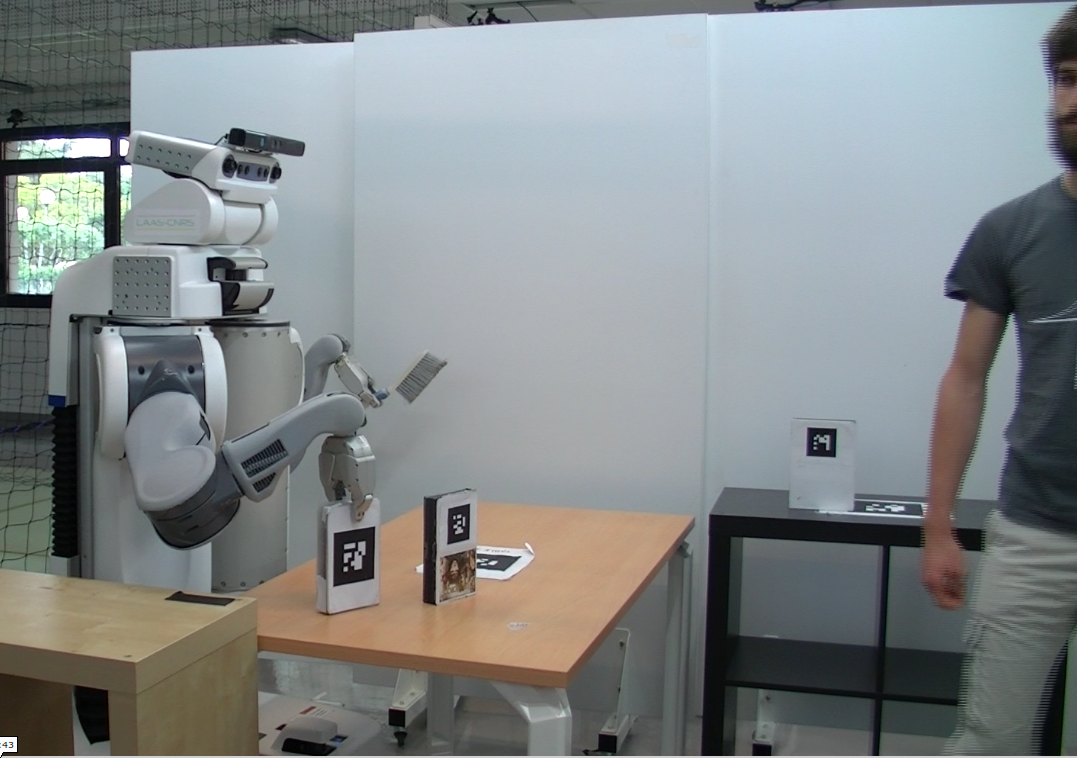
\includegraphics[width=0.4\textwidth]{figs/Chapter3/HumanLeave.png}
       \label{subfig:humanLeave}
   }
    %~
    \subfigure[The robot removes the last book and sweep the table.]{
        \centering
        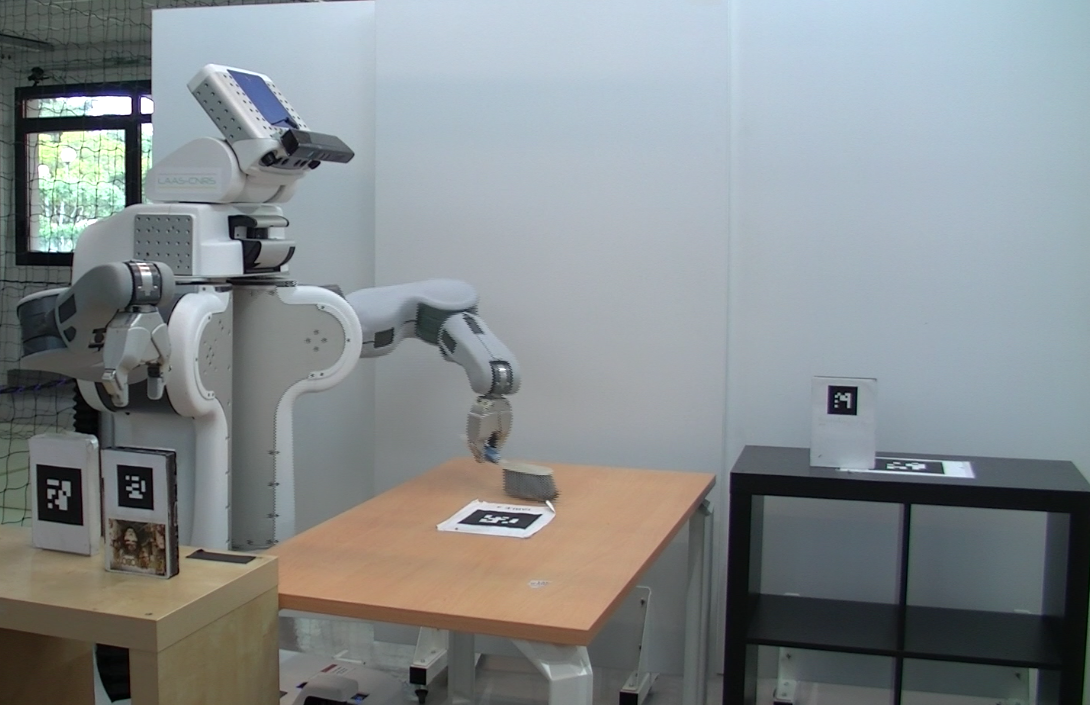
\includegraphics[width=0.44\textwidth]{figs/Chapter3/robotSweep.png}
       \label{subfig:robotSweep}
    }
    %~
    \subfigure[The human comes back.]{
        \centering
        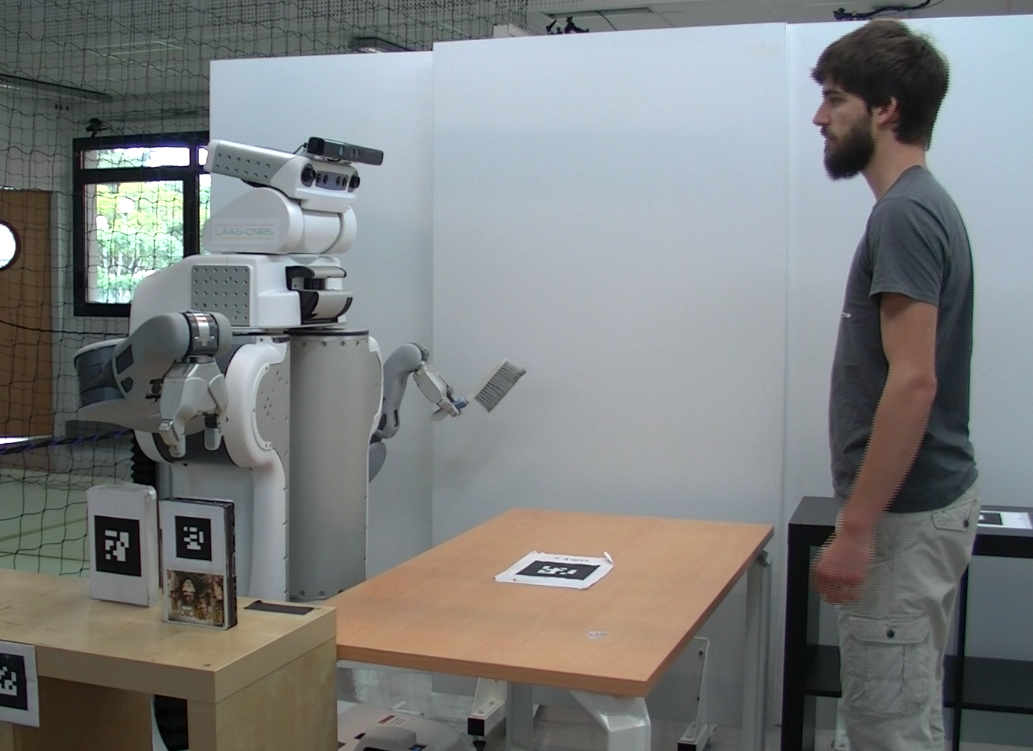
\includegraphics[width=0.4\textwidth]{figs/Chapter3/humanComesBack.png}
       \label{subfig:humanComesBack}
   }
    %~
    \subfigure[The human and the robot perform their last actions and achieve the task.]{
        \centering
        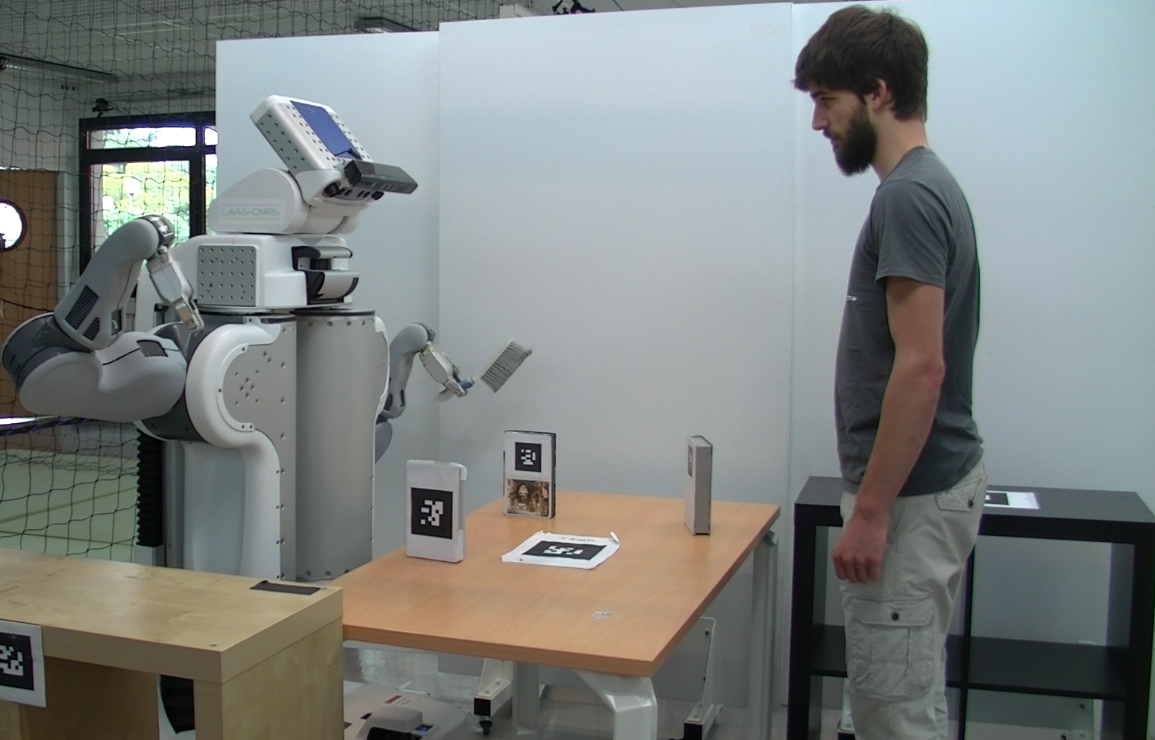
\includegraphics[width=0.45\textwidth]{figs/Chapter3/endClean.png}
       \label{subfig:endClean}
    }
    \caption{Illustrative "Clean the table" scenario.}
\end{figure*}

\subsection{Quantitative results}

We will now evaluate the benefits of the presented work in simulation in the two tasks described previously. Results in real situations as well as more simulation results with the whole system developed in the thesis can be found in Chapter~\ref{ch:Eval}). The results here only concern the use of mental states during Shared Plan execution.

When the interaction starts, we consider that the joint goal is already established and that a first Shared Plan has been computed by the robot. The robot executes the plan and the simulated human executes the actions planned for him. We randomly sample a time when the human leaves the scene and another time when the human comes back. While absent, the human does not execute actions and cannot see anything nor communicate.

One objective of our contribution is to reduce unnecessary communication from the robot during the execution of a Shared Plan aiming at a more friendly and less intrusive behavior of the robot. Consequently, in order to evaluate our system, we have chosen to measure the amount of information shared by the robot during a Shared Plan execution. During the interaction, we logged the number of facts (information chunks) given by the robot to the human. An information concerns either a change in the environment or the state of a previous action. 

We compared our system (called \textit{ToM system}) to:
\begin{itemize}
\item a system which informs about each action missed by the human (called \textit{Missed system}).
\item a system which informs about each action performed by the robot even if the human sees it (called \textit{Performed system}).
\end{itemize}

The obtained results in 100 runs are given in Table~\ref{table:results}.

We can see that our system allows to reduce significantly the amount of information given by the robot. In the "Clean the table" scenario, depending on when the human leaves, the robot might change the initial plan and take care of the book reachable by both agents instead of the human. This explains why the average number for the \textit{Performed system} is higher than the number of actions initially planned for the robot: the robot performs more actions in the new plan. In this scenario, our system allows not to communicate about missed \textit{pickandplace} actions as the human can infer them by looking at the objects placements. However, the robot will inform the human if he missed the fact that the robot has swept the table as it is not observable and it is a necessary information for the human to know before he can put back objects on the table.

\begin{table}[ht]
\begin{center}
\begin{tabular}{|r||c|c||c|c|}
\hline
 Scenario & \multicolumn{2}{c||}{Clean the table} & \multicolumn{2}{c|}{Inventory}\\
\cline{2-5} 
System & Average & Std Dev & Average & Std Dev\\
\hline
\hline
ToM & 0.94 & 0.24 & 0.41 & 0.48\\
\hline
Missed & 2.14 & 0.87 & 2.61 & 1.36\\
\hline
Performed & 3.72 & 0.96 & 10.0 & 0.0\\
\hline
\end{tabular}
\end{center}
\caption{Number of information given by the robot during the two presented scenarios for the three systems (\textit{TOM}, \textit{Missed} and \textit{Performed}).}
\label{table:results}
\end{table}

In the inventory scenario, as all objects and boxes are reachable only by one agent, the robot does not change the plan when the human leaves. This explains the fact that the standard deviation is null for the \textit{Performed system}: the number of actions performed by the robot never changes and there is no change in the plan. In this scenario, the \textit{pickanddrop} and \textit{scan} actions have non-observable effects (the human can not see an object in a box). However, we can see that our system still verbalizes less information than the \textit{Missed system}: the robot communicates only the information which the human really needs (as the fact that an object the human should drop in a box has been scanned) and does not give information which are not linked to the human part of the plan (as the fact that the robot scanned an object it have to drop in its box or that the robot dropped an object).


\section{Conclusion}

In this chapter we showed how we extended the robot estimation of humans mental states (which initially concerned only the environment) to the state of the task and more specifically of the Shared Plan. Then, we showed how we use these mental states to better communicate during Shared Plan execution.

The benefits of this work have been demonstrated with an illustrative example and simulation results. These results show that the proposed system allows to reduce communication by removing useless information given by the robot.

The next chapter will give more details about Shared Plan elaboration and management, more particularly concerning actions allocation. Then, we will show in Chapter~\ref{ch:Eval}) more complete simulation results with the whole system as well as results with the system running in a real situation.

\ifdefined\included
\else
\bibliographystyle{StyleThese}
\bibliography{These}
\end{document}
\fi

\ifdefined\included
\else
\documentclass[english,a4paper,11pt,twoside]{StyleThese}
\usepackage{amsmath,amssymb}             % AMS Math
\usepackage[T1]{fontenc}
\usepackage[utf8x]{inputenc}
\usepackage{babel}
\usepackage{datetime}

\usepackage{lmodern}
\usepackage{tabularx}
%\usepackage{tabular}
\usepackage{multirow}

\usepackage{subfigure}
\usepackage{fancyvrb}
\usepackage{algorithmic}
\usepackage{algorithm}
\usepackage{mathtools}


\usepackage{hhline}
\usepackage[left=1.5in,right=1.3in,top=1.1in,bottom=1.1in,includefoot,includehead,headheight=13.6pt]{geometry}
\renewcommand{\baselinestretch}{1.05}

% Table of contents for each chapter

\usepackage[nottoc, notlof, notlot]{tocbibind}
\usepackage{minitoc}
\setcounter{minitocdepth}{2}
\mtcindent=15pt
% Use \minitoc where to put a table of contents

\usepackage{aecompl}


% Glossary / list of abbreviations

\usepackage[intoc]{nomencl}
\iftoggle{ThesisInEnglish}{%
\renewcommand{\nomname}{Glossary}
}{ %
\renewcommand{\nomname}{Liste des Abréviations}
}

\newcommand{\accom}[1]{\textcolor{red}{[#1]}}

\makenomenclature

% My pdf code

\usepackage{ifpdf}

\ifpdf
  \usepackage[pdftex]{graphicx}
  \DeclareGraphicsExtensions{.jpg}
  \usepackage[a4paper,pagebackref,hyperindex=true]{hyperref}
  \usepackage{tikz}
  \usetikzlibrary{arrows,shapes,calc}
\else
  \usepackage{graphicx}
  \DeclareGraphicsExtensions{.ps,.eps}
  \usepackage[a4paper,dvipdfm,pagebackref,hyperindex=true]{hyperref}
\fi

\graphicspath{{.}{images/}}

%% nicer backref links. NOTE: The flag ThesisInEnglish is used to define the
% language in the back references. Read more about it in These.tex

\iftoggle{ThesisInEnglish}{%
\renewcommand*{\backref}[1]{}
\renewcommand*{\backrefalt}[4]{%
\ifcase #1 %
(Not cited.)%
\or
(Cited in page~#2.)%
\else
(Cited in pages~#2.)%
\fi}
\renewcommand*{\backrefsep}{, }
\renewcommand*{\backreftwosep}{ and~}
\renewcommand*{\backreflastsep}{ and~}
}{%
\renewcommand*{\backref}[1]{}
\renewcommand*{\backrefalt}[4]{%
\ifcase #1 %
(Non cité.)%
\or
(Cité en page~#2.)%
\else
(Cité en pages~#2.)%
\fi}
\renewcommand*{\backrefsep}{, }
\renewcommand*{\backreftwosep}{ et~}
\renewcommand*{\backreflastsep}{ et~}
}

% Links in pdf
\usepackage{color}
\definecolor{linkcol}{rgb}{0,0,0.4} 
\definecolor{citecol}{rgb}{0.5,0,0} 
\definecolor{linkcol}{rgb}{0,0,0} 
\definecolor{citecol}{rgb}{0,0,0}
% Change this to change the informations included in the pdf file

\hypersetup
{
bookmarksopen=true,
pdftitle="Joint Action for Human-Robot Interaction",
pdfauthor="Sandra DEVIN", %auteur du document
pdfsubject="Thesis", %sujet du document
%pdftoolbar=false, %barre d'outils non visible
pdfmenubar=true, %barre de menu visible
pdfhighlight=/O, %effet d'un clic sur un lien hypertexte
colorlinks=true, %couleurs sur les liens hypertextes
pdfpagemode=None, %aucun mode de page
pdfpagelayout=SinglePage, %ouverture en simple page
pdffitwindow=true, %pages ouvertes entierement dans toute la fenetre
linkcolor=linkcol, %couleur des liens hypertextes internes
citecolor=citecol, %couleur des liens pour les citations
urlcolor=linkcol %couleur des liens pour les url
}

% definitions.
% -------------------

\setcounter{secnumdepth}{3}
\setcounter{tocdepth}{2}

% Some useful commands and shortcut for maths:  partial derivative and stuff

\newcommand{\pd}[2]{\frac{\partial #1}{\partial #2}}
\def\abs{\operatorname{abs}}
\def\argmax{\operatornamewithlimits{arg\,max}}
\def\argmin{\operatornamewithlimits{arg\,min}}
\def\diag{\operatorname{Diag}}
\newcommand{\eqRef}[1]{(\ref{#1})}

\usepackage{rotating}                    % Sideways of figures & tables
%\usepackage{bibunits}
%\usepackage[sectionbib]{chapterbib}          % Cross-reference package (Natural BiB)
%\usepackage{natbib}                  % Put References at the end of each chapter
                                         % Do not put 'sectionbib' option here.
                                         % Sectionbib option in 'natbib' will do.
\usepackage{fancyhdr}                    % Fancy Header and Footer

% \usepackage{txfonts}                     % Public Times New Roman text & math font
  
%%% Fancy Header %%%%%%%%%%%%%%%%%%%%%%%%%%%%%%%%%%%%%%%%%%%%%%%%%%%%%%%%%%%%%%%%%%
% Fancy Header Style Options

\pagestyle{fancy}                       % Sets fancy header and footer
\fancyfoot{}                            % Delete current footer settings

%\renewcommand{\chaptermark}[1]{         % Lower Case Chapter marker style
%  \markboth{\chaptername\ \thechapter.\ #1}}{}} %

%\renewcommand{\sectionmark}[1]{         % Lower case Section marker style
%  \markright{\thesection.\ #1}}         %

\fancyhead[LE,RO]{\bfseries\thepage}    % Page number (boldface) in left on even
% pages and right on odd pages
\fancyhead[RE]{\bfseries\nouppercase{\leftmark}}      % Chapter in the right on even pages
\fancyhead[LO]{\bfseries\nouppercase{\rightmark}}     % Section in the left on odd pages

\let\headruleORIG\headrule
\renewcommand{\headrule}{\color{black} \headruleORIG}
\renewcommand{\headrulewidth}{1.0pt}
\usepackage{colortbl}
\arrayrulecolor{black}

\fancypagestyle{plain}{
  \fancyhead{}
  \fancyfoot{}
  \renewcommand{\headrulewidth}{0pt}
}

%\usepackage{MyAlgorithm}
%\usepackage[noend]{MyAlgorithmic}
\usepackage[ED=MITT - STICIA, Ets=INP]{tlsflyleaf}
%%% Clear Header %%%%%%%%%%%%%%%%%%%%%%%%%%%%%%%%%%%%%%%%%%%%%%%%%%%%%%%%%%%%%%%%%%
% Clear Header Style on the Last Empty Odd pages
\makeatletter

\def\cleardoublepage{\clearpage\if@twoside \ifodd\c@page\else%
  \hbox{}%
  \thispagestyle{empty}%              % Empty header styles
  \newpage%
  \if@twocolumn\hbox{}\newpage\fi\fi\fi}

\makeatother
 
%%%%%%%%%%%%%%%%%%%%%%%%%%%%%%%%%%%%%%%%%%%%%%%%%%%%%%%%%%%%%%%%%%%%%%%%%%%%%%% 
% Prints your review date and 'Draft Version' (From Josullvn, CS, CMU)
\newcommand{\reviewtimetoday}[2]{\special{!userdict begin
    /bop-hook{gsave 20 710 translate 45 rotate 0.8 setgray
      /Times-Roman findfont 12 scalefont setfont 0 0   moveto (#1) show
      0 -12 moveto (#2) show grestore}def end}}
% You can turn on or off this option.
% \reviewtimetoday{\today}{Draft Version}
%%%%%%%%%%%%%%%%%%%%%%%%%%%%%%%%%%%%%%%%%%%%%%%%%%%%%%%%%%%%%%%%%%%%%%%%%%%%%%% 

\newenvironment{maxime}[1]
{
\vspace*{0cm}
\hfill
\begin{minipage}{0.5\textwidth}%
%\rule[0.5ex]{\textwidth}{0.1mm}\\%
\hrulefill $\:$ {\bf #1}\\
%\vspace*{-0.25cm}
\it 
}%
{%

\hrulefill
\vspace*{0.5cm}%
\end{minipage}
}

\let\minitocORIG\minitoc
\renewcommand{\minitoc}{\minitocORIG \vspace{1.5em}}

\usepackage{multirow}
%\usepackage{slashbox}

\newenvironment{bulletList}%
{ \begin{list}%
	{$\bullet$}%
	{\setlength{\labelwidth}{25pt}%
	 \setlength{\leftmargin}{30pt}%
	 \setlength{\itemsep}{\parsep}}}%
{ \end{list} }

\newtheorem{definition}{Définition}
\renewcommand{\epsilon}{\varepsilon}

% centered page environment

\newenvironment{vcenterpage}
{\newpage\vspace*{\fill}\thispagestyle{empty}\renewcommand{\headrulewidth}{0pt}}
{\vspace*{\fill}}

\usepackage{tablefootnote}

\sloppy
\begin{document}
\setcounter{chapter}{3} %% Numéro du chapitre précédent ;)
\dominitoc
\faketableofcontents
\fi

\chapter{When to take decisions during Shared Plans elaboration and execution}
\minitoc

\label{ch:SP}

\section{Motivation}

When performing a Joint Action and more particularly when executing Shared Plans, several choices have to be made. Some of them are implicit, while others require a negotiation or an adaptation between the Joint Action participants. To be a good partner when performing Joint Action with humans, the robot should be able to identify which decisions are implicit and correctly communicate about the other ones. Indeed, a robot which communicates about each detail of a Shared Plan would easily become too "chatty" when a robot which does not communicate can be confusing.

Let's take for example a robot helping a human to build a flat-pack table: the legs of the table need to be assembled with a hammer, the tray with a screwdriver and finally someone needs to put the tray on the legs. The robot is equipped with several tools including a screwdriver but no hammer and the human has only one hammer. The human and the robot are both able to put the tray on the legs. It is common sense that the robot should assemble the tray while the human assemble the legs. However, a decision needs to be taken concerning who will put the tray on the legs. 
In this scenario, the robot should assemble the tray without asking the human and negotiate or adapt its behavior to put the tray. 

The work presented in this chapter consists in finding which decisions are implicit or not, when the decisions should be taken and how to take them. We identify three types of decisions to be taken during Shared Plans elaboration and execution:
\begin{itemize}
\item \textbf{Which action to perform in which order:} this is one of the biggest concern during Shared Plan elaboration. We do not focus our work in this part. Indeed, we use for this part HATP, a human-aware HTN planner which has been demonstrated to be well suited to human-robot joint action \cite{Lallement2014hatp}.
\item \textbf{Who will perform which action:} sometimes this decision can be implicit when only one agent is able to perform an action. However, in other situations, the robot should be able to decide who will perform an action by negotiating or adapting its behavior to the human one.
\item \textbf{With which object:} for practical reason, the robot reasons on objects by attributing them a unique id. However, for the purpose of an action, two objects can be semantically identical. When there is a choice in which object to use for an action, the robot should be able to adapt to the human behavior in order to avoid potential conflicts.
\end{itemize}

\section{Background}

When the robot needs to achieve a joint goal, several works allow it to compute plans which take into account the human (\cite{cirillo2010human,Lallement2014hatp}). They allow the robot to reduce resource conflicts \cite{chakraborti2016planning}, take divergent beliefs into account (\cite{guitton2012belief,talamadupula2014coordination}) or promote stigmergic collaboration
for agents in co-habitation \cite{chakraborti2015planning}. 

The relevance of using a Shared Plan in human-robot interaction has been studied by \cite{lallee2013cooperative}. They suggest that the joint plan should be fully communicated in order to sustain effective collaboration. Moreover, in \cite{gombolay2015decision}, it is shown that subjects prefer letting the robot plan when the task is too complex, prioritizing efficiency. 
In more simple tasks, a robot proactively helping the human is preferred to one waiting before proposing help \cite{baraglia2016initiative}. 

If the robot decides to share the plan, several studies have been reported on how to do communicate about the plan. Some researchers studied how a system could acquire knowledge on plan decomposition from a user \cite{Mohseni2015} and how dialog can be used to teach new collaborative plans to the robot and to modify these plans \cite{petit2013coordinating}. In \cite{sorce2015proof}, the system is able to learn a plan from a user and transmit it to another user. \cite{allen2002human} presents a computer agent able to construct a plan in collaboration with a user. Finally, in \cite{milliez2016using}, Milliez et al. present a system where the robot shares the plan with a level of details which depends on the expertise of the user. In our work, we try to get rid of the entire shared plan verbalization by taking the right decision at the right time in order to come up with a robot which communicates at the right time.

Several contributions have been done to allow more adaptability during shared plan execution. \cite{chien2000using} proposes a method to plan only a few steps in advance and then plan the actions further in an iterative way. Chaski, a task-level
executive, presented in \cite{shah2011improved}, allows to choose when to execute the robot actions adapting to a human partner. A system which mixes plan recognition and adaptation is described in \cite{levine2014concurrent}. It computes all possibilities for the plan and chooses an action based on the choice of the human and causal links. \cite{hoffman2007effects} proposes an adaptive action selection mechanism for a robotic teammate, making anticipatory decisions based on the confidence of their validity and their relative risk. \cite{karpas2015robust} presents Pike, an online executive that unifies intent recognition and plan adaptation for temporally flexible plans with choice. Finally, this work is based on SHARY \cite{clodic2009shary} which was extended in \cite{fiore2014planning}, a supervisor allowing to execute human-aware shared plans taking into account joint actions aspects like reactive action execution.

In the cooperative multi-robot literature, task allocation and cooperative activity achievement has been thoroughly investigated \cite{gerkey2004formal}. Auction has been used very successfully for distributed multi-robot in various contexts (\cite{gerkey2002sold,botelho1999m+}). 
Concerning the so-called teamwork and cooperative task achievement taking into account explicit constraints to facilitate the activity of the other robots or agents activity, one can mention \cite{tambe1997agent} and \cite{joyeux2009plan}. While these contributions have inspired work on human-robot collaboration, it is however important to exhibit some differences between the two fields. Indeed, the human and the robot are not equal in any aspect. The robot is here to help the human and facilitate his activity.

In AI, the goal reasoning domains deals with some problems similar to Shared Plan management \cite{molineaux2010goal, roberts2016goal}. The role of goal reasoning is to survey the current goals of a robot, check that they remain feasible and relevant and establish new goals if needed. Moreover, part of the goal reasoning function is sometimes linked to the plan management as it is in charge of deciding when and how to generate plans (but it is not producing the plan) and checking for unexpected events. 

\section{Assumptions}

The work presented in this chapter treats of the needed decision during Shared Plan elaboration and execution. The focus is put here into the decisions concerning the action allocation and instantiation. To do so, we make several assumptions:

\paragraph{Single human:} the work presented in this chapter has been designed for a robot interacting with a single human. However, all the data structures and main principles are compatible with multi-humans set-up.

\paragraph{Commitment:} we do not focus in this works on issues related to commitment. Consequently, we consider here that the joint goal has already been established. We also consider that the human will not abort the goal unless he knows that the goal is not achievable any more.

\paragraph{Shared Plan:} we put the focus here on the issues related to action allocation and instantiation. In order to decide which action to execute in which order, we use HATP, a human-aware HTN planner which has been demonstrated to be well suited to human-robot Joint Action \cite{Lallement2014hatp}.
We are focusing in this work about medium complexity Shared Plans where the human might want to decide for his own actions.

\paragraph{Humans perception:} we make the assumption here that a human will see and understand an action of the robot when he is present and looking at it. We also assume that when he is present, the human is able to hear and understand the information verbalized by the robot.

\paragraph{Robot capacities:} we consider that the robot is able to perform simple high level actions like Pick, Place or Drop. We also assume that the robot is able to ask to the human if he wants to perform an action and to understand a basic answer (yes/no type). 
The robot is able to detect and localize objects and agents
and to recognize simple high level actions performed by the human like Pick, Place or Drop. Let us also note that the ways the robot achieves actions (e.g. human-aware motion planning and execution) and recognizes human's actions are outside of the scope of this chapter.

\paragraph{Communication:} the focus of this work is more on the what to communicate and when than on the how to communicate. Here we use the basic dialogue module described in Chapter~\ref{ch:Sup} to communicate with the human but more complex communication mechanisms can be envisioned. 

\section{Main principles}

We will present in this section the main principles we use for Shared Plans management. Three algorithms are used to allow the robot to elaborate and execute Shared Plans.  They interact through the Shared Plan data \textit{SP} and several signals (noted \textit{S\_X} where \textit{X} is the name of the signal). These three algorithm run constantly and in parallel.They allow respectively to maintain the state of the shared plan, to choose actions for the robot, and to monitor the human.

The Alg.~\ref{alg:mainPlan} allows the robot to elaborate a Shared Plan when needed, to maintain the current Shared Plan and to manage the human mental states. The terms used in the algorithms are reminded in Appendix \ref{chap:annexe1}.

\begin{algorithm}
\caption{Shared Plan management}
\label{alg:mainPlan}
\begin{algorithmic}
\WHILE {$g_R$}
\IF {$!SP \ \| \ S\_needReplan$}
\STATE $SP \leftarrow PLAN(g_R, WS)$
\ENDIF
\IF {S\_needUpdate}
\STATE $SP \leftarrow UPDATE\_PLAN(SP, WS)$
\ENDIF
\IF {S\_actionAllocated}
\STATE $SP \leftarrow EVALUATE\_ PLAN(SP, WS)$
\ENDIF
\IF {$Obj_g \in WS$ \hfill \textit{$\vartriangleright$ The goal is achieved}
\STATE}
\STATE $g_R \leftarrow \emptyset$ 
\STATE $SP \leftarrow \emptyset$
\ENDIF
\IF {$<Human, isPresent, true> \in WS \ \& \ (WS(H) \neq WS(H)_{t-1} \  \|  \  TS \neq TS_{t-1})$}
\STATE $MS(H) \leftarrow ESTIMATE\_MS(MS(H), TS)$
\IF {$MS(H) \neq TS$ \hfill \textit{$\vartriangleright$ Divergent belief}
\STATE}
\STATE $SOLVE\_DB(MS(H), TS)$
\ENDIF
\ENDIF
\ENDWHILE
\end{algorithmic}
\end{algorithm} 

When the robot has a goal $g_R$ to achieve and no current plan or when a signal is received to compute a new plan ($S\_needReplan$), the robot computes a Shared Plan to perform the goal based on the current world state $WS$ (see Sec.~\ref{sec:elaboration}):
$$SP \leftarrow PLAN(g_R, WS)$$

When an action $a$ from the plan is performed by an agent a signal is received ($S\_needUpdate$) and the robot updates the plan (see Sec.~\ref{subsec:maintaining}):
$$SP \leftarrow UPDATE\_PLAN(SP, a)$$

When an action from $A^X$ has been allocated ($S\_actionAllocated$), the robot looks for the consequences of this allocation in the plan (see Sec.~\ref{subsec:allocation}):
$$SP \leftarrow EVALUATE\_ PLAN(SP, WS)$$
The robot also constantly checks if the goal is reached (the objectives of the goal are in the current World State).
Finally, each time a change occurs in $WS(H)$ or $TS$, the robot estimates the human mental states as described in the previous chapter (see Chapter~\ref{ch:MS}):
$$MS(H) \leftarrow ESTIMATE\_MS(MS(H), TS)$$
If there is a conflict between the knowledge of the robot and the human mental state, the robot tries to solve it (see Chapter~\ref{ch:MS}): 
$$SOLVE\_DB(MS(H), TS)$$

In parallel to the first algorithm, Alg.~\ref{alg:mainExec} allows the robot to decide when to act and which action to perform. 


\begin{algorithm}
\caption{Robot action decision}
\label{alg:mainExec}
\begin{algorithmic}
\WHILE {$SP$}
\STATE $A_{next} \leftarrow GET\_NEXT\_ACTIONS(SP, WS)$
\IF {$A_{next} = \emptyset$ \hfill \textit{$\vartriangleright$ No more feasible actions}
\STATE}
\STATE $S\_needReplan$
\ELSIF {$\{A^R_{next} \cup A^X_{next}\} =  \emptyset$ \hfill \textit{$\vartriangleright$ No actions for the robot
\STATE}}
\STATE $actionExecuted \leftarrow WAIT\_ACTION(A^H_{next}, t)$
\IF {!actionExecuted}
\STATE $S\_needReplan$
\ENDIF 
\ELSE
\STATE $a \leftarrow SELECT\_ACTION\_TODO(A_{next})$
\IF {$a \in A^X_{next}$}
\STATE $actor \leftarrow ALLOCATE\_ACTION(SP, a, WS, Prefs)$
\STATE $S\_actionAllocated$
\ENDIF
\IF {$a \in A^R_{next} \ \| \ (a \in A^X_{next} \ \& \ actor = robot)$}
\STATE $success \leftarrow EXECUTE(a)$
\IF {success}
\STATE $S\_needUpdate$
\ELSE 
\STATE $S\_needReplan$
\ENDIF
\ELSIF {$(a \in A^X_{next} \ \& \ actor = human)$}
\STATE $a \rightarrow A^H_{next}$
\ENDIF
\ENDIF
\ENDWHILE
\end{algorithmic}
\end{algorithm} 

When the robot has a Shared Plan $SP$, it looks for the action of this plan which need to and can be executed (see Sec. \ref{subsec:maintaining}):
$$A_{next} \leftarrow GET\_NEXT\_ACTIONS(SP, WS)$$
If there is no action in $A_{next}$ nor in progress, it means that the plan is blocked, so the robot looks for another Shared Plan. If there are actions to do, the robot looks if there is an action it can execute (actions allocated to it or not allocated yet). If there is none, the robot waits for the human to perform an action ($A_{next}$ contains only actions from $A^H_{next}$):
$$actionExecuted \leftarrow WAIT\_ACTION(A^H_{next}, t)$$
If after a time \textit{t}, the human did not execute any action, the robot looks for another plan.
If there are actions the robot can execute, the robot selects an action $a$ (see Sec. \ref{subsec:selection}):
$$a \leftarrow SELECT\_ACTION\_TODO(A_{next})$$
If the selected action is not yet allocated, the robot first tries to allocate it (see Sec. \ref{subsec:allocation}):
$$actor \leftarrow ALLOCATE\_ACTION(SP, a, WS, Prefs)$$
If the action is allocated to the robot (after selection or allocation), the robot executes it:
$$success \leftarrow EXECUTE(a)$$
It will first instantiate the action if needed and then launch its execution (see Sec. \ref{subsec:execution}). If the action succeeds, the robot updates the plan, else it looks for another plan.

In parallel to the other execution loops, the robot is constantly monitoring human activities (Alg.~\ref{alg:monitoring}).

\begin{algorithm}
\caption{Human monitoring}
\label{alg:monitoring}
\begin{algorithmic}
\WHILE {$<Human, isPresent, true> \in WS$}
\IF {$\exists \ a \in A^H_{cur}$}
\IF {$a \in A^R_{cur}$}
\STATE $S\_stop$
\ENDIF
\STATE WAIT\_END\_ACTION(a)
\IF {$a \in A^H_{next}$}
\STATE $S\_needUpdate$
\ELSIF {$a \in A^X_{now}$}
\STATE $S\_actionAllocated$
\ELSE 
\STATE $S\_needReplan$ \hfill \textit{$\vartriangleright$ Unexpected action}
\ENDIF
\ENDIF
\ENDWHILE
\end{algorithmic}
\end{algorithm}

When the human performs an action, the robot first looks if the action is concurrent to the one it is performing (for example, if the human picks an object the robot was going to pick), and if it is the case, the robot stops its actions.  
Then, if the human performs an expected action with respect to the plan and already allocated to him, the robot updates the plan accordingly. If the action executed by the human is expected with respect to the plan but was not yet allocated, the robot looks for the consequences of this actions in the plan (see Sec. \ref{subsec:allocation}).
If the human performs an unexpected action with respect to the plan (action not in $A_{next}$ or in $A^R_{next}$), the robot looks for a new plan from the new situation induced by the human action.

The next sections will define more precisely the operators we just defined.


\section{Shared Plans elaboration}

\label{sec:elaboration}

The first step of this work is to be able to compute Shared Plans flexible enough to let part of the decisions to execution time. This step correspond to the operator:
$$PLAN(g_R, WS)$$

As stated before, the human-aware HTN task planner HATP is used in this work to compute Shared Plans taking into account a number of social rules for both the robot and its human partner \cite{Lallement2014hatp}. However, in order to obtain flexible plans with HATP, a number of issues have to be considered.

First, when HATP returns a plan, it returns only one, which is assumed to be the best plan it has found given the situation and the associated costs. However, this plan is not always the only one possible (even at constant cost or computing time). Indeed, in such case, HATP makes some choices that could be preferably done on-line. For example, it can happen that one action can be done by several agents at the same cost. In a collaborative setting and more particularly when the human is concerned, it could be interesting to let the agents decide at execution time (or whenever it is interesting) who will do what. To handle this, we have adapted HATP by inserting what we call the\textit{X agent}. The capabilities of the \textit{X agent} correspond to the intersection of the capabilities of the human and the robot with a lower cost. Consequently, it will be chosen by the planner instead of the human or the robot whenever it is possible. If HATP returns a plan containing an action to be done by the \textit{X agent}, it means that this action could either be performed by the human or the robot. The decision concerning who will finally do this action is postponed. We will see in Sec. \ref{subsec:allocation} how \textit{X agent} actions will be finally allocated to the human or the robot.

As inputs to a planner such as HATP, we give a set of objects that are present in the environment and on which it will be able to apply its operators. Basically, each object is tagged and is unique. That means that if we have the same object twice, they will be uniquely tagged (e.g. two identical red cubes will be tagged as RED\_CUBE\_1 and RED\_CUBE\_2). When two similar objects can be used in a same way during a task, the planner will choose either one or the other. In a collaborative setting, it could be counter intuitive since even if there is no distinction between the two objects at planning time, there can be one during execution. To handle this, we have adapted HATP by inserting the notion of \textit{similar} objects which aims to group interchangeable objects under a common name: two \textit{similar} objects will have the same role in the task. 

Finally, rather than in other works where we used HATP, we do not consider here that an agent is only capable to perform one action at a time. This allows the human to choose the order of his action when there is no impact in the global plan.

\section{Shared Plans execution}

We will now see in more detail how the robot executes the flexible Shared Plans obtained.

\subsection{Plan maintaining}
\label{subsec:maintaining}

First, the robot needs to be able to follow the Shared Plan execution and to determine which actions need to be executed and which actions need to be left for later. 

As said before, the actions composing a Shared Plan can be decomposed as:
$$A_p = <A_{prev}, A_{cur}, A_{next}, A_{later}>$$

By default, when a Shared Plan is computed by the robot, all actions are put in $A_{later}$. When the robot performs an action or detects an action execution from a human, the executed action goes in $A_{cur}$ and, at the end of the execution, the action goes in $A_{prev}$ with a label equal either to DONE if the execution has been successful, FAILED if not or ABORTED if the robot had to stop the execution for an external reason.

An action will be put in $A_{next}$ if all previous actions in the plan are DONE (based on causal links) and its preconditions are checked:

$$a \in A_{next} \Leftrightarrow Precs_{a} \in WS \ \& \ (\forall l \in L_p \ | \ next_l = id_a,$$ 
$$\exists \ ap \in A_{prev} \ | \ (id_{ap} = prev_l \ \& \ label_{ap}  = DONE))$$

The $UPDATE\_PLAN$ operator updates the state of each action of the plan and the $GET\_NEXT\_ACTIONS$ operator returns the actions in $A_{next}$.


\subsection{Action selection}
\label{subsec:selection}

Once the robot knows which actions need to be executed, it needs to choose one from the set of actions it can execute. To do so, it uses the $SELECT\_ACTION\_TODO$ operator which returns the action with the higher priority:

$$\underset{a \in \{A^R_{next} \cup A^X_{next}\}}{\mathrm{argmax}} \ priority(a)$$

\textbf{Priorities used:}
In our case, we have chosen to give higher priority to the actions allocated to the robot compared to those not already allocated. In general for this work, we have made the choice to postpone as much as possible the decisions made by the robot. Indeed, this choice is made in order to give as much latitude as possible to the human, which allows him to take the initiative until the last possible moment. In the current implementation of our system, the priorities of the different actions of the robot are the same, so the robot will simply select one. However, there is a possibility to later integrate costs as, for example, select the action the farthest of what the human is currently doing. Concerning the priorities of not allocated actions, we still follow the principle to postpone as much as possible the robot decision. To do so, we put a higher priority on what we call \textit{analogous} actions. Two actions will be \textit{analogous} when they have exactly the same decomposition (same action name and same parameters). Indeed, as there is several time the action to execute, putting a higher priority on \textit{analogous} actions allows to robot to execute one (and advance in the plan) while letting to the human the possibility to perform the other one.

\subsection{Action allocation}
\label{subsec:allocation}

Once a not yet allocated action is selected, the robot needs to decide if it should execute it or not ($ALLOCATE\_ACTION$ operator). To do so, the robot first looks for the possible actors of this action: agents which verify the preconditions of the action and which are not already busy. Note that even if the action was not allocated by HATP it is possible that there is only one possible actor. In this case, the robot automatically allocates the action to this agent. For example if the human is currently busy and there is a not allocated action  to perform, the robot will execute it. If there is more than one possible actor for the action, the robot follows the algorithm \ref{alg:allocate}.

\begin{algorithm}
\caption{Action allocation: $SP \leftarrow ALLOCATE\_ACTION(SP, a, WS, Prefs)$}
\label{alg:allocate}
\begin{algorithmic}
\REQUIRE $a \in A^X_{next}$
\IF {$cost(a, R) << cost(a, H)$}
\STATE $actor \leftarrow robot$
\ELSIF {$cost(a, H) << cost(a, R)$}
\STATE $actor \leftarrow human$
\ELSIF {mode = negotiation}
\STATE $answer \leftarrow ASK(a, H)$
\IF {answer = yes}
\STATE $actor \leftarrow human$
\ELSE
\STATE $actor \leftarrow robot$
\ENDIF
\ELSE
\STATE $actionPerformed \leftarrow WAIT\_ACTION(a, t)$
\hfill \textit{$\vartriangleright$ adaptation mode}
\IF {$actionPerformed$}
\STATE $actor \leftarrow human$
\ELSE
\STATE $actor \leftarrow robot$
\ENDIF
\ENDIF
\RETURN $actor$
\end{algorithmic}
\end{algorithm}

First, the robot compares the estimated cost for the human and for itself to perform the action. If it considers it significantly more costly for the human to perform the action, it will allocate the action to itself. Then, we have developed two possible modes for the robot. In the first mode, called \textbf{negotiation} mode, the robot directly asks its human partner if he wants to perform the action and then allocates the action according to his answer. In the other mode, called \textbf{adaptation} mode, the robot waits a certain amount of time, and, if the human does not take the initiative to perform the action, it executes it. 

Allocating an action to an agent can lead to other actions being automatically allocated. For this reason, after each allocation of an action, a new plan is built taking into account the possible allocations of the actions remaining in $A_X$.

\textbf{Costs used for action selection ($cost(a, R)$ and $cost(a, H)$):}
In the current implementation, we use a cost concerning the \textit{analogous} actions (see description in the previous subsection). These \textit{analogous} actions will have a lower cost for the robot to execute them leading the robot to automatically execute one of them. Indeed, as there is several time the same action to perform, the robot can execute one while letting to the human the possibility to perform the other(s).

Other costs can be considered as human preferences. We can imagine having a list of actions the human likes to perform and another he dislikes. The robot can then allocate the actions following these preferences.

\subsection{Action execution}
\label{subsec:execution}

Once the robot has decided to execute an action ($EXECUTE$ operator), it needs to be able to deal with the \textit{similar} objects introduced before. To do so, we keep the principle that the robot waits until the last moment to take a decision. For example, if the robot and the human have to pick objects and place them in several similar placements, the robot will first pick an object and only after choose a placement to place it. Then, when the robot has to choose an object, it will choose the one it considers the less costly.

Finally, if the human approaches an object which is involved in the current robot action (e.g. if he places an object in a placement the robot chose), the robot first halts its action. Then, the robot looks if it can find another \textit{similar} object. If it finds one, it continues its action with this object. If not, it waits for the human to retreat from the object, and if the human actions did not lead to a new plan it continues its action if possible.

\textbf{Costs used for objects selection:}
Here we choose to put a lower cost on objects accessible only by the robot (we still want to let the maximum choices to the human). Then, we use a simple cost based on distance. In our cost, we get the distances between the agents hands (here we have chosen the right hand) and objects. For objects accessible only by the robot the costs will be proportional to the distance between the robot hand and the objects, leading the robot to choose the closest one. Concerning objects accessible also by the human, the costs will be inversely proportional to the distance between the human hand and the objects, leading the robot to choose the farthest object from the human to minimize the efforts for the human to reach the objects left. 


\section{Results}

\subsection{Task}

To illustrate the work done in this chapter, we use a task adapted for the manipulation abilities of a PR2 robot and inspired from the one in \cite{clodic2014key}. A human and a robot have to build a blocks construction as represented in Fig. \ref{subfig:goal}. At the beginning of the task, the robot and the human have several colored blocks they can access as in Fig. \ref{subfig:setUp}. Two identical placements are set on the table to indicate where to put the two red cubes.

\begin{figure*}[!h]
\centering
	\subfigure[Goal of the task (side view)]{
        \centering
        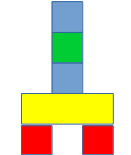
\includegraphics[width=0.25\textwidth]{figs/Chapter4/BlockGoal.png}
       \label{subfig:goal}
   }
    %~
	\subfigure[One possible initial set-up (top view)]{
        \centering
        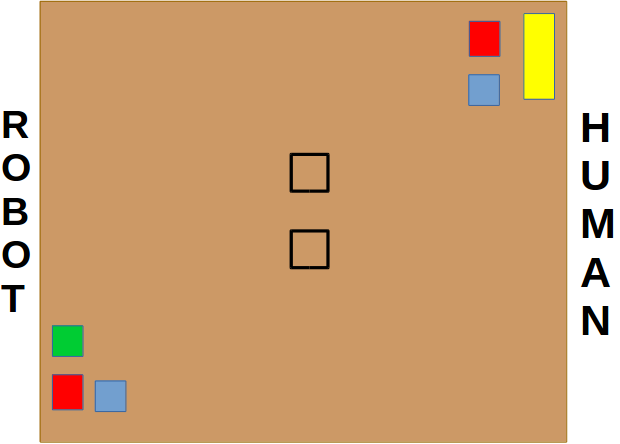
\includegraphics[width=0.4\textwidth]{figs/Chapter4/SetUp.png}
       \label{subfig:setUp}
   }
    \caption{Description of the blocks building task. The human and the robot have to build the stack together. We assume that the robot and the human know where all the available blocks are. We would like the robot to adapt as much as possible to the human actions and decisions while avoiding useless or tiresome verbal interactions}
    \label{fig:blocksBuildingTask}
\end{figure*}

\subsection{Illustrative example}

We will first present one possible scenario of the task described earlier which illustrate well the benefits of this work.

\begin{figure*}[!h]
\centering
	\subfigure[Initial plan]{
        \centering
        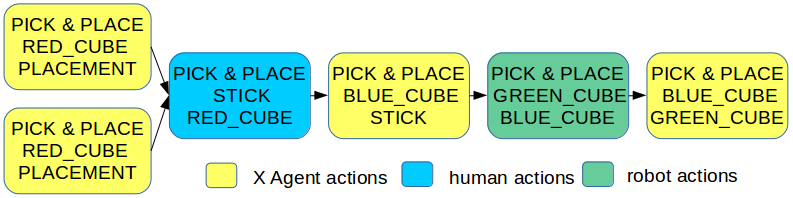
\includegraphics[width=0.7\textwidth]{figs/Chapter4/init_plan.png}
       \label{subfig:initPlan}
   }
    %~
	\subfigure[The robot chooses to put the red cube in the placement to its right]{
        \centering
        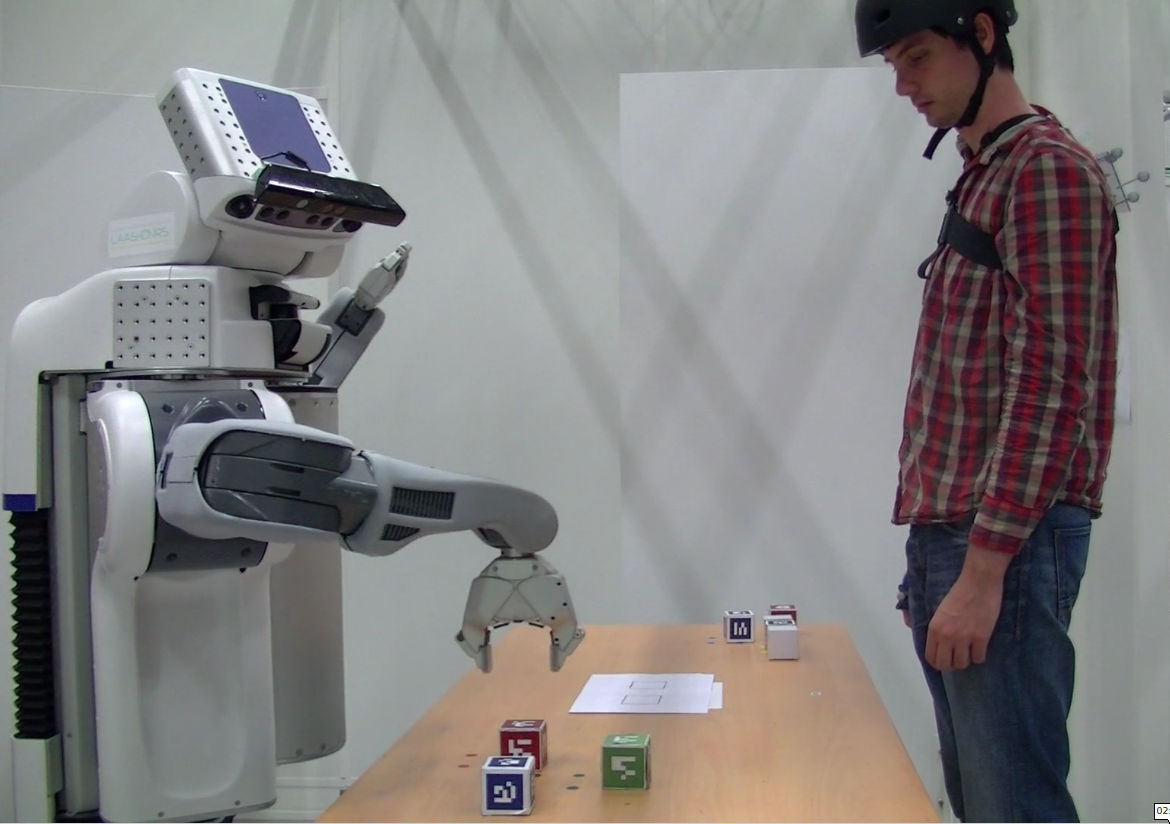
\includegraphics[width=0.4\textwidth]{figs/Chapter4/screen_shot1.jpeg}
       \label{subfig:redCube}
   }
    %~
	\subfigure[The human places his cube in the placement the robot chose]{
        \centering
        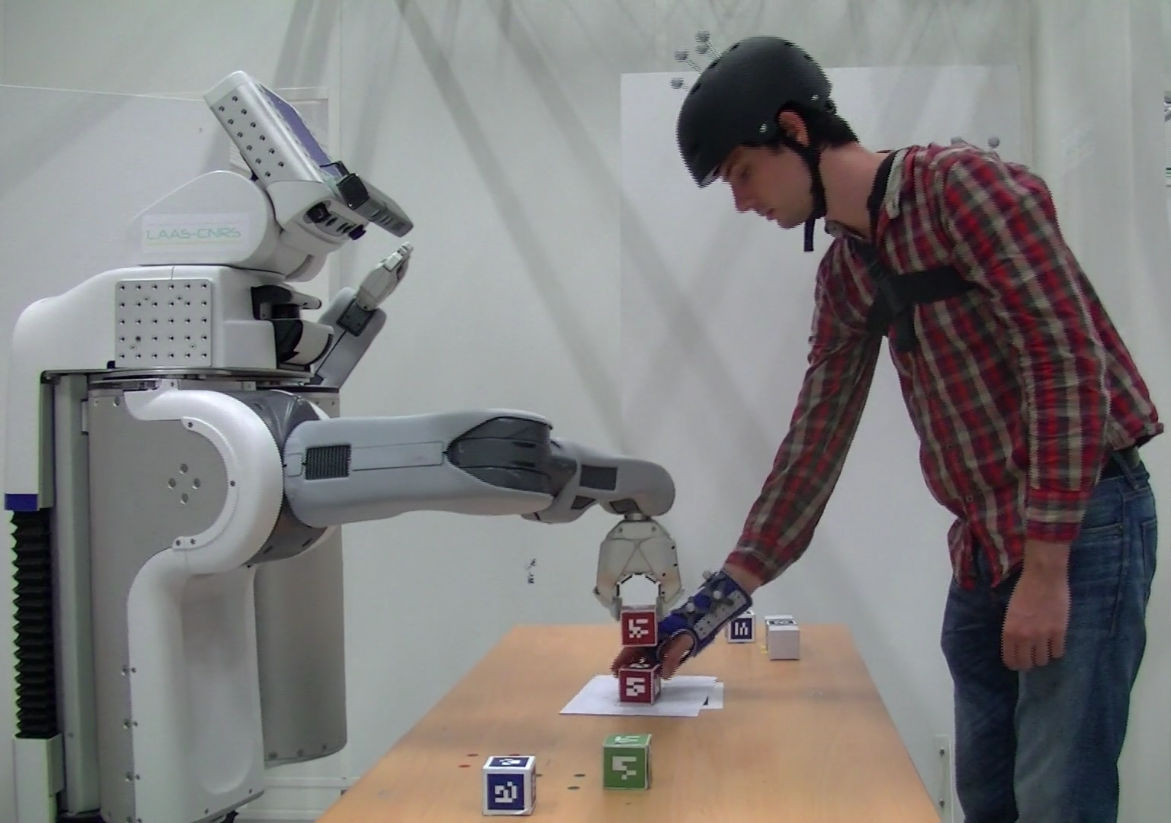
\includegraphics[width=0.4\textwidth]{figs/Chapter4/screen_shot2.jpeg}
       \label{subfig:humanPlace}
   }
    %~
	\subfigure[Second computed plan]{
        \centering
        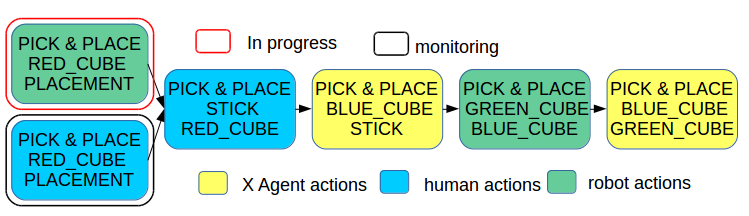
\includegraphics[width=0.7\textwidth]{figs/Chapter4/second_plan.png}
       \label{subfig:secondPlan}
   }
    %~
	\subfigure[The robot adapts by changing its placement choice]{
        \centering
        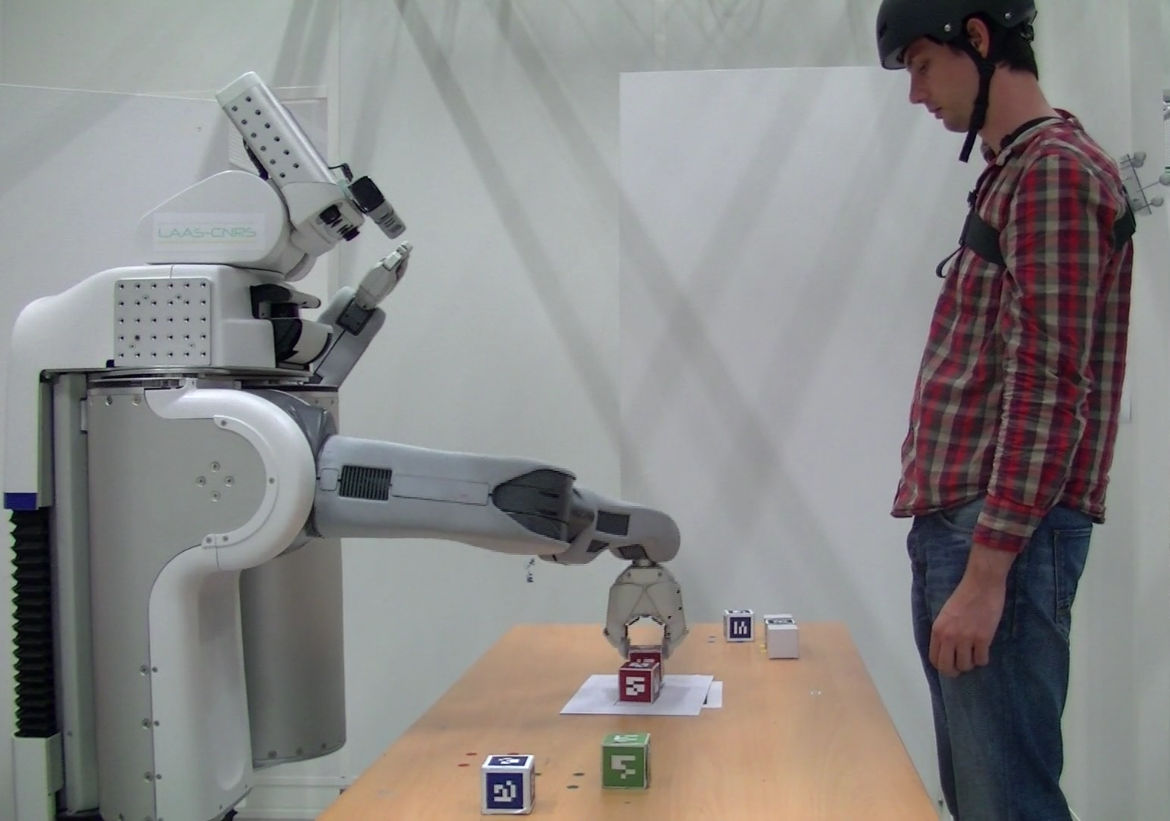
\includegraphics[width=0.4\textwidth]{figs/Chapter4/screen_shot3.jpeg}
       \label{subfig:robotAdapts}
   }
    %~
	\subfigure[Third computed plan]{
        \centering
        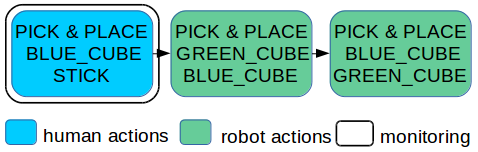
\includegraphics[width=0.4\textwidth]{figs/Chapter4/third_plan.png}
       \label{subfig:thirdPlan}
   }
    \caption{The human and the robot build a blocks construction together. The robot adapts its behavior to the human actions.}
\end{figure*}


The presented scenario starts with the set-up in Fig.~\ref{subfig:setUp}. The plan produced by HATP for this set-up can be found in Fig.~\ref{subfig:initPlan}. As this plan starts with two \textit{analogous} actions for the \textit{X agent} (place a red cube into a placement), the robot selects one and starts to execute it. So, the robot picks the red cube (Fig. \ref{subfig:redCube}) and, at the same time, looks for the consequences of its choice in the plan. As both agents own only one red cube, in the new plan computed by the robot (Fig.~\ref{subfig:secondPlan}) the human needs to place the second red cube. After picking its red cube the robot starts to place it on the placement to its right. However, the human picks his red cube and places it in the very same placement (Fig.~\ref{subfig:humanPlace}). So, the robot stops its movement and adapts by placing its cube in the other placement (Fig.~\ref{subfig:robotAdapts}). Then, the human places the stick on the red cubes. In this scenario, we have chosen to set the robot into the \textbf{negotiation} mode. As the next action is allocated to the \textit{X agent}, the robot asks the human if he wants to do it (\textit{"Do you want to place the blue cube?"}). The human answers yes, leading the robot to compute the new plan in Fig.~\ref{subfig:thirdPlan} where the human have to place the first blue cube and the robot the second one. Finally, the human and the robot perform their last actions and achieve the goal.


\subsection{Quantitative results}

In order to evaluate our system, we run it in simulation using the blocks building scenario. Different set-ups were used as initial state of the task: we randomized the number of cubes of each color in the environment and their position (accessible by the robot or the human). The robot was confronted to a simulated human with different types of behaviors:

\begin{itemize}
\item \textbf{The "kind" human:} this human performs all actions that are feasible only by him and, when there is an action feasible by both him and the robot, he either chooses to perform it with 50 \% chance (noted "50\%-K"), systematically chooses to perform it (noted "hurry-K") or systematically chooses not to perform it (noted "lazy-K"). The "kind" human answers to robot questions and adapts his behavior to what the robot verbalizes (he does an action if the robot asks him and stops his action if the robot says it will perform it).
\item \textbf{The "stubborn" human:} contrary to the "kind" human, this human does not react nor comply to robot verbalization: he will not change his decision to perform or not an action (noted "50\%-S", "hurry-S" and "lazy-S").
\end{itemize}

We compare the two different modes of our system ("negotiation" and "adaptation", see Sec.~\ref{subsec:allocation}) to a reference system (RS) where the Shared Plans are completely refined during plan elaboration (no \textit{X agent} nor \textit{similar} object). Concerning what the robot says, we choose to run the reference system with three different modes:
\begin{itemize}
\item the robot verbalizes nothing (noted "RS-none").
\item the robot informs the human when he has to perform an action (noted "RS-human").
\item the robot informs the human when he has to perform an action and when it will act (noted "RS-all").
\end{itemize}

We measured the number of verbal interactions between the human and the robot (Tab.~\ref{tab:incompatible}) and the number of human/robot incompatible decisions (Tab.~\ref{tab:incompatible}): either both decide to perform the same action (and the robot stops its own action to avoid the conflict) or both decide not to perform the action (the robot first asks the human to perform the action after a predefined time and, if after another period the human has still not executed the action, the robot looks for a new plan where it can proceed).

\begin{table*}[!h]
  \begin{tabular}{|c||c|c|c|c|c||}
  \hline
     & \textbf{RS-none} & \textbf{RS-human} & \textbf{RS-all} & \textbf{Neg} & \textbf{Adapt} \\
  \hline
  \hline
     \textbf{50\%-K} & 0.6 & 0.1 & 0.0 & 0.0 & 0.0 \\
     \textbf{(SD)} & (0.52) & (0.32) & (0.0) & (0.0) & (0.0) \\
  \hline
     \textbf{hurry-K} & 0.3 & 0.3 & 0.0 & 0.0 & 0.0 \\
     \textbf{(SD)} & (0.48) & (0.48) & (0.0) & (0.0) & (0.0) \\
  \hline
     \textbf{lazy-K} & 0.9) & 0.0 & 0.0 & 0.0 & 0.0 \\
     \textbf{(SD)} & (0.32) & (0.0) & (0.0) & (0.0) & (0.0) \\
  \hline
     \textbf{50\%-S} & 0.5 & 0.7 & 0.6 & 0.0 & 0.0 \\
     \textbf{(SD)} & (0.53) & (0.67) & (0.52) & (0.0) & (0.0) \\
  \hline
     \textbf{hurry-S} & 0.3 & 0.3 & 0.3 & 0.0 & 0.0 \\
     \textbf{(SD)} & (0.48) & (0.48) & (0.48) & (0.0) & (0.0) \\
  \hline
     \textbf{lazy-S} & 0.9 & 0.9 & 0.9 & 0.0 & 0.0 \\
     \textbf{(SD)} & (0.32) & (0.32) & (0.32) & (0.0) & (0.0) \\
  \hline
  \end{tabular}
   \caption{Results for the reference system (RS) and the proposed system (Neg for the negotiation mode and Adapt for the adaptation mode). Number of incompatible decisions between the human and the robot (i.e. either both agents decide to perform the same action or both decide not to perform a given action). The numbers correspond to means in 10 runs and their associated standard deviations.}
   \label{tab:incompatible} 
\end{table*}

We also measured execution time but no significant difference was found between the different conditions. Indeed, this criterion is not pertinent here since, as all actions concern the same stack, they need to be performed one after the other. Consequently, there is no significant difference time between the different options.

\begin{table*}[!h]
  \begin{tabular}{|c||c|c|c|c|c||}
  \hline
     & \textbf{RS-none} & \textbf{RS-human} & \textbf{RS-all} & \textbf{Neg} & \textbf{Adapt} \\
  \hline
  \hline
     \textbf{50\%-K} & 0.4 & 2.1 & 5.1 & 1.2 & 0.0 \\
     \textbf{(SD)} & (0.52) & (0.32) & (0.32) & (0.63) & (0.0) \\
  \hline
     \textbf{hurry-K} & 0.0 & 2.1 & 5.1 & 1.2 & 0.0 \\
     \textbf{(SD)} & (0.0) & (0.32) & (0.32) & (0.63) & (0.0) \\
  \hline
     \textbf{lazy-K} & 0.9 & 2.1 & 5.1 & 1.2 & 0.0 \\
     \textbf{(SD)} & (0.32) & (0.32) & (0.32) & (0.63) & (0.0) \\
  \hline
     \textbf{50\%-S} & 0.4 & 2.1 & 5.1 & 1.2 & 0.0 \\
     \textbf{(SD)} & (0.52) & (0.32) & (0.32) & (0.63) & (0.0) \\
  \hline
     \textbf{hurry-S} & 0.0 & 2.1 & 5.1 & 1.2 & 0.0) \\
     \textbf{(SD)} & (0.0) & (0.32) & (0.32) & (0.63) & (0.0) \\
  \hline
     \textbf{lazy-S} & 0.9 & 2.1 & 5.1 & 1.2 & 0.0 \\
     \textbf{(SD)} & (0.32) & (0.32) & (0.32) & (0.63) & (0.0) \\
  \hline
  \end{tabular}
   \caption{Results for the reference system (RS) and the proposed system (Neg for the negotiation mode and Adapt for the adaptation mode). Number of verbal interactions (i.e. question asked by the robot in the negotiation mode or an information given with the reference system). The numbers correspond to means in 10 runs and their associated standard deviations.}
   \label{tab:verb}
\end{table*}

We can see that with the reference system, even when the human is "kind", the less the robot speaks, the more there are incompatible decisions between the human and the robot. Indeed, with this system, as the robot decides in advance the actions allocation, it needs to inform the human in order for him to adapt to the robot plan. It is worse when the human is "stubborn" since, even if the robot informs the human, the conflicts remain. Note that even in the case where the robot was not supposed to verbalize anything (RS-none), there is still verbalization: this is due to the incompatible decisions where the human and the robot both choose not to execute the action, the robot tries to solve the conflict by asking the human to execute the action.

With our new system, we can see that the robot is able to avoid conflicts in all cases without being too talkative (or without being talkative at all for the adaptation mode). This system allows more freedom to the human by letting him the choice to perform or not actions: with the "stubborn" human who performs the actions he wants to perform the robot still avoids conflicts without having to be more "chatty" (this is not the case with the reference system).

Finally, here the adaptation mode performs better than the negotiation one since the human is simulated and always performs his actions in time. However, in a real context, the negotiation mode could have the benefit to ensure the absence of conflicts even if the robot is a little more talkative. Moreover, the human can be more comfortable with a robot which directly asks when (and only when) there is a decision to take compared to a robot which has unnecessary waiting time. Such measure of "satisfaction" will be treated in Chapter~\ref{ch:Eval} where a study with real participants has been made.

\section{Conclusion}

In this chapter we shown how we enable the robot to compute and execute more flexible Shared Plans. In these new plans, the needed decisions on who will execute an action and with which objects are let to the execution. A number of the presented algorithms involve cost estimation in order to decide between options. In the current system, simple costs are used but could be easily replaced by more elaborate ones. For instance, a finer estimation of action costs based on geometric reasoning and human efforts would allow better informed choice for action or object selection. Another interesting issue would be to integrate the estimation of accumulated costs of all actions remaining in the plan.

The benefits of this work have been demonstrated with an illustrative example and simulation results. We will show in Chapter~\ref{ch:Eval}) more complete simulation results which also include the work of the previous chapter as well as results with the system running in a real situation.


\ifdefined\included
\else
\bibliographystyle{StyleThese}
\bibliography{These}
\end{document}
\fi

\ifdefined\included
\else
\documentclass[english,a4paper,11pt,twoside]{StyleThese}
\usepackage{amsmath,amssymb}             % AMS Math
\usepackage[T1]{fontenc}
\usepackage[utf8x]{inputenc}
\usepackage{babel}
\usepackage{datetime}

\usepackage{lmodern}
\usepackage{tabularx}
%\usepackage{tabular}
\usepackage{multirow}

\usepackage{subfigure}
\usepackage{fancyvrb}
\usepackage{algorithmic}
\usepackage{algorithm}
\usepackage{mathtools}


\usepackage{hhline}
\usepackage[left=1.5in,right=1.3in,top=1.1in,bottom=1.1in,includefoot,includehead,headheight=13.6pt]{geometry}
\renewcommand{\baselinestretch}{1.05}

% Table of contents for each chapter

\usepackage[nottoc, notlof, notlot]{tocbibind}
\usepackage{minitoc}
\setcounter{minitocdepth}{2}
\mtcindent=15pt
% Use \minitoc where to put a table of contents

\usepackage{aecompl}


% Glossary / list of abbreviations

\usepackage[intoc]{nomencl}
\iftoggle{ThesisInEnglish}{%
\renewcommand{\nomname}{Glossary}
}{ %
\renewcommand{\nomname}{Liste des Abréviations}
}

\newcommand{\accom}[1]{\textcolor{red}{[#1]}}

\makenomenclature

% My pdf code

\usepackage{ifpdf}

\ifpdf
  \usepackage[pdftex]{graphicx}
  \DeclareGraphicsExtensions{.jpg}
  \usepackage[a4paper,pagebackref,hyperindex=true]{hyperref}
  \usepackage{tikz}
  \usetikzlibrary{arrows,shapes,calc}
\else
  \usepackage{graphicx}
  \DeclareGraphicsExtensions{.ps,.eps}
  \usepackage[a4paper,dvipdfm,pagebackref,hyperindex=true]{hyperref}
\fi

\graphicspath{{.}{images/}}

%% nicer backref links. NOTE: The flag ThesisInEnglish is used to define the
% language in the back references. Read more about it in These.tex

\iftoggle{ThesisInEnglish}{%
\renewcommand*{\backref}[1]{}
\renewcommand*{\backrefalt}[4]{%
\ifcase #1 %
(Not cited.)%
\or
(Cited in page~#2.)%
\else
(Cited in pages~#2.)%
\fi}
\renewcommand*{\backrefsep}{, }
\renewcommand*{\backreftwosep}{ and~}
\renewcommand*{\backreflastsep}{ and~}
}{%
\renewcommand*{\backref}[1]{}
\renewcommand*{\backrefalt}[4]{%
\ifcase #1 %
(Non cité.)%
\or
(Cité en page~#2.)%
\else
(Cité en pages~#2.)%
\fi}
\renewcommand*{\backrefsep}{, }
\renewcommand*{\backreftwosep}{ et~}
\renewcommand*{\backreflastsep}{ et~}
}

% Links in pdf
\usepackage{color}
\definecolor{linkcol}{rgb}{0,0,0.4} 
\definecolor{citecol}{rgb}{0.5,0,0} 
\definecolor{linkcol}{rgb}{0,0,0} 
\definecolor{citecol}{rgb}{0,0,0}
% Change this to change the informations included in the pdf file

\hypersetup
{
bookmarksopen=true,
pdftitle="Joint Action for Human-Robot Interaction",
pdfauthor="Sandra DEVIN", %auteur du document
pdfsubject="Thesis", %sujet du document
%pdftoolbar=false, %barre d'outils non visible
pdfmenubar=true, %barre de menu visible
pdfhighlight=/O, %effet d'un clic sur un lien hypertexte
colorlinks=true, %couleurs sur les liens hypertextes
pdfpagemode=None, %aucun mode de page
pdfpagelayout=SinglePage, %ouverture en simple page
pdffitwindow=true, %pages ouvertes entierement dans toute la fenetre
linkcolor=linkcol, %couleur des liens hypertextes internes
citecolor=citecol, %couleur des liens pour les citations
urlcolor=linkcol %couleur des liens pour les url
}

% definitions.
% -------------------

\setcounter{secnumdepth}{3}
\setcounter{tocdepth}{2}

% Some useful commands and shortcut for maths:  partial derivative and stuff

\newcommand{\pd}[2]{\frac{\partial #1}{\partial #2}}
\def\abs{\operatorname{abs}}
\def\argmax{\operatornamewithlimits{arg\,max}}
\def\argmin{\operatornamewithlimits{arg\,min}}
\def\diag{\operatorname{Diag}}
\newcommand{\eqRef}[1]{(\ref{#1})}

\usepackage{rotating}                    % Sideways of figures & tables
%\usepackage{bibunits}
%\usepackage[sectionbib]{chapterbib}          % Cross-reference package (Natural BiB)
%\usepackage{natbib}                  % Put References at the end of each chapter
                                         % Do not put 'sectionbib' option here.
                                         % Sectionbib option in 'natbib' will do.
\usepackage{fancyhdr}                    % Fancy Header and Footer

% \usepackage{txfonts}                     % Public Times New Roman text & math font
  
%%% Fancy Header %%%%%%%%%%%%%%%%%%%%%%%%%%%%%%%%%%%%%%%%%%%%%%%%%%%%%%%%%%%%%%%%%%
% Fancy Header Style Options

\pagestyle{fancy}                       % Sets fancy header and footer
\fancyfoot{}                            % Delete current footer settings

%\renewcommand{\chaptermark}[1]{         % Lower Case Chapter marker style
%  \markboth{\chaptername\ \thechapter.\ #1}}{}} %

%\renewcommand{\sectionmark}[1]{         % Lower case Section marker style
%  \markright{\thesection.\ #1}}         %

\fancyhead[LE,RO]{\bfseries\thepage}    % Page number (boldface) in left on even
% pages and right on odd pages
\fancyhead[RE]{\bfseries\nouppercase{\leftmark}}      % Chapter in the right on even pages
\fancyhead[LO]{\bfseries\nouppercase{\rightmark}}     % Section in the left on odd pages

\let\headruleORIG\headrule
\renewcommand{\headrule}{\color{black} \headruleORIG}
\renewcommand{\headrulewidth}{1.0pt}
\usepackage{colortbl}
\arrayrulecolor{black}

\fancypagestyle{plain}{
  \fancyhead{}
  \fancyfoot{}
  \renewcommand{\headrulewidth}{0pt}
}

%\usepackage{MyAlgorithm}
%\usepackage[noend]{MyAlgorithmic}
\usepackage[ED=MITT - STICIA, Ets=INP]{tlsflyleaf}
%%% Clear Header %%%%%%%%%%%%%%%%%%%%%%%%%%%%%%%%%%%%%%%%%%%%%%%%%%%%%%%%%%%%%%%%%%
% Clear Header Style on the Last Empty Odd pages
\makeatletter

\def\cleardoublepage{\clearpage\if@twoside \ifodd\c@page\else%
  \hbox{}%
  \thispagestyle{empty}%              % Empty header styles
  \newpage%
  \if@twocolumn\hbox{}\newpage\fi\fi\fi}

\makeatother
 
%%%%%%%%%%%%%%%%%%%%%%%%%%%%%%%%%%%%%%%%%%%%%%%%%%%%%%%%%%%%%%%%%%%%%%%%%%%%%%% 
% Prints your review date and 'Draft Version' (From Josullvn, CS, CMU)
\newcommand{\reviewtimetoday}[2]{\special{!userdict begin
    /bop-hook{gsave 20 710 translate 45 rotate 0.8 setgray
      /Times-Roman findfont 12 scalefont setfont 0 0   moveto (#1) show
      0 -12 moveto (#2) show grestore}def end}}
% You can turn on or off this option.
% \reviewtimetoday{\today}{Draft Version}
%%%%%%%%%%%%%%%%%%%%%%%%%%%%%%%%%%%%%%%%%%%%%%%%%%%%%%%%%%%%%%%%%%%%%%%%%%%%%%% 

\newenvironment{maxime}[1]
{
\vspace*{0cm}
\hfill
\begin{minipage}{0.5\textwidth}%
%\rule[0.5ex]{\textwidth}{0.1mm}\\%
\hrulefill $\:$ {\bf #1}\\
%\vspace*{-0.25cm}
\it 
}%
{%

\hrulefill
\vspace*{0.5cm}%
\end{minipage}
}

\let\minitocORIG\minitoc
\renewcommand{\minitoc}{\minitocORIG \vspace{1.5em}}

\usepackage{multirow}
%\usepackage{slashbox}

\newenvironment{bulletList}%
{ \begin{list}%
	{$\bullet$}%
	{\setlength{\labelwidth}{25pt}%
	 \setlength{\leftmargin}{30pt}%
	 \setlength{\itemsep}{\parsep}}}%
{ \end{list} }

\newtheorem{definition}{Définition}
\renewcommand{\epsilon}{\varepsilon}

% centered page environment

\newenvironment{vcenterpage}
{\newpage\vspace*{\fill}\thispagestyle{empty}\renewcommand{\headrulewidth}{0pt}}
{\vspace*{\fill}}

\usepackage{tablefootnote}

\sloppy
\begin{document}
\setcounter{chapter}{4} %% Numéro du chapitre précédent ;)
\dominitoc
\faketableofcontents
\fi

\chapter{Communicating during Shared Plans Execution: what should the robot do with its head?}
\minitoc

\label{ch:Acting}

\section{Motivations}

\section{Background}

\section{Identifications of needed signals}

\section{Unitary evaluation of signals}

\section{\textcolor{red}{Proposed system}}

\section{\textcolor{red}{Results}}

\ifdefined\included
\else
\bibliographystyle{StyleThese}
\bibliography{These}
\end{document}
\fi


\part{Other contributions on Human-Robot Joint Action}

\ifdefined\included
\else
\documentclass[english,a4paper,11pt,twoside]{StyleThese}
\usepackage{amsmath,amssymb}             % AMS Math
\usepackage[T1]{fontenc}
\usepackage[utf8x]{inputenc}
\usepackage{babel}
\usepackage{datetime}

\usepackage{lmodern}
\usepackage{tabularx}
%\usepackage{tabular}
\usepackage{multirow}

\usepackage{subfigure}
\usepackage{fancyvrb}
\usepackage{algorithmic}
\usepackage{algorithm}
\usepackage{mathtools}


\usepackage{hhline}
\usepackage[left=1.5in,right=1.3in,top=1.1in,bottom=1.1in,includefoot,includehead,headheight=13.6pt]{geometry}
\renewcommand{\baselinestretch}{1.05}

% Table of contents for each chapter

\usepackage[nottoc, notlof, notlot]{tocbibind}
\usepackage{minitoc}
\setcounter{minitocdepth}{2}
\mtcindent=15pt
% Use \minitoc where to put a table of contents

\usepackage{aecompl}


% Glossary / list of abbreviations

\usepackage[intoc]{nomencl}
\iftoggle{ThesisInEnglish}{%
\renewcommand{\nomname}{Glossary}
}{ %
\renewcommand{\nomname}{Liste des Abréviations}
}

\newcommand{\accom}[1]{\textcolor{red}{[#1]}}

\makenomenclature

% My pdf code

\usepackage{ifpdf}

\ifpdf
  \usepackage[pdftex]{graphicx}
  \DeclareGraphicsExtensions{.jpg}
  \usepackage[a4paper,pagebackref,hyperindex=true]{hyperref}
  \usepackage{tikz}
  \usetikzlibrary{arrows,shapes,calc}
\else
  \usepackage{graphicx}
  \DeclareGraphicsExtensions{.ps,.eps}
  \usepackage[a4paper,dvipdfm,pagebackref,hyperindex=true]{hyperref}
\fi

\graphicspath{{.}{images/}}

%% nicer backref links. NOTE: The flag ThesisInEnglish is used to define the
% language in the back references. Read more about it in These.tex

\iftoggle{ThesisInEnglish}{%
\renewcommand*{\backref}[1]{}
\renewcommand*{\backrefalt}[4]{%
\ifcase #1 %
(Not cited.)%
\or
(Cited in page~#2.)%
\else
(Cited in pages~#2.)%
\fi}
\renewcommand*{\backrefsep}{, }
\renewcommand*{\backreftwosep}{ and~}
\renewcommand*{\backreflastsep}{ and~}
}{%
\renewcommand*{\backref}[1]{}
\renewcommand*{\backrefalt}[4]{%
\ifcase #1 %
(Non cité.)%
\or
(Cité en page~#2.)%
\else
(Cité en pages~#2.)%
\fi}
\renewcommand*{\backrefsep}{, }
\renewcommand*{\backreftwosep}{ et~}
\renewcommand*{\backreflastsep}{ et~}
}

% Links in pdf
\usepackage{color}
\definecolor{linkcol}{rgb}{0,0,0.4} 
\definecolor{citecol}{rgb}{0.5,0,0} 
\definecolor{linkcol}{rgb}{0,0,0} 
\definecolor{citecol}{rgb}{0,0,0}
% Change this to change the informations included in the pdf file

\hypersetup
{
bookmarksopen=true,
pdftitle="Joint Action for Human-Robot Interaction",
pdfauthor="Sandra DEVIN", %auteur du document
pdfsubject="Thesis", %sujet du document
%pdftoolbar=false, %barre d'outils non visible
pdfmenubar=true, %barre de menu visible
pdfhighlight=/O, %effet d'un clic sur un lien hypertexte
colorlinks=true, %couleurs sur les liens hypertextes
pdfpagemode=None, %aucun mode de page
pdfpagelayout=SinglePage, %ouverture en simple page
pdffitwindow=true, %pages ouvertes entierement dans toute la fenetre
linkcolor=linkcol, %couleur des liens hypertextes internes
citecolor=citecol, %couleur des liens pour les citations
urlcolor=linkcol %couleur des liens pour les url
}

% definitions.
% -------------------

\setcounter{secnumdepth}{3}
\setcounter{tocdepth}{2}

% Some useful commands and shortcut for maths:  partial derivative and stuff

\newcommand{\pd}[2]{\frac{\partial #1}{\partial #2}}
\def\abs{\operatorname{abs}}
\def\argmax{\operatornamewithlimits{arg\,max}}
\def\argmin{\operatornamewithlimits{arg\,min}}
\def\diag{\operatorname{Diag}}
\newcommand{\eqRef}[1]{(\ref{#1})}

\usepackage{rotating}                    % Sideways of figures & tables
%\usepackage{bibunits}
%\usepackage[sectionbib]{chapterbib}          % Cross-reference package (Natural BiB)
%\usepackage{natbib}                  % Put References at the end of each chapter
                                         % Do not put 'sectionbib' option here.
                                         % Sectionbib option in 'natbib' will do.
\usepackage{fancyhdr}                    % Fancy Header and Footer

% \usepackage{txfonts}                     % Public Times New Roman text & math font
  
%%% Fancy Header %%%%%%%%%%%%%%%%%%%%%%%%%%%%%%%%%%%%%%%%%%%%%%%%%%%%%%%%%%%%%%%%%%
% Fancy Header Style Options

\pagestyle{fancy}                       % Sets fancy header and footer
\fancyfoot{}                            % Delete current footer settings

%\renewcommand{\chaptermark}[1]{         % Lower Case Chapter marker style
%  \markboth{\chaptername\ \thechapter.\ #1}}{}} %

%\renewcommand{\sectionmark}[1]{         % Lower case Section marker style
%  \markright{\thesection.\ #1}}         %

\fancyhead[LE,RO]{\bfseries\thepage}    % Page number (boldface) in left on even
% pages and right on odd pages
\fancyhead[RE]{\bfseries\nouppercase{\leftmark}}      % Chapter in the right on even pages
\fancyhead[LO]{\bfseries\nouppercase{\rightmark}}     % Section in the left on odd pages

\let\headruleORIG\headrule
\renewcommand{\headrule}{\color{black} \headruleORIG}
\renewcommand{\headrulewidth}{1.0pt}
\usepackage{colortbl}
\arrayrulecolor{black}

\fancypagestyle{plain}{
  \fancyhead{}
  \fancyfoot{}
  \renewcommand{\headrulewidth}{0pt}
}

%\usepackage{MyAlgorithm}
%\usepackage[noend]{MyAlgorithmic}
\usepackage[ED=MITT - STICIA, Ets=INP]{tlsflyleaf}
%%% Clear Header %%%%%%%%%%%%%%%%%%%%%%%%%%%%%%%%%%%%%%%%%%%%%%%%%%%%%%%%%%%%%%%%%%
% Clear Header Style on the Last Empty Odd pages
\makeatletter

\def\cleardoublepage{\clearpage\if@twoside \ifodd\c@page\else%
  \hbox{}%
  \thispagestyle{empty}%              % Empty header styles
  \newpage%
  \if@twocolumn\hbox{}\newpage\fi\fi\fi}

\makeatother
 
%%%%%%%%%%%%%%%%%%%%%%%%%%%%%%%%%%%%%%%%%%%%%%%%%%%%%%%%%%%%%%%%%%%%%%%%%%%%%%% 
% Prints your review date and 'Draft Version' (From Josullvn, CS, CMU)
\newcommand{\reviewtimetoday}[2]{\special{!userdict begin
    /bop-hook{gsave 20 710 translate 45 rotate 0.8 setgray
      /Times-Roman findfont 12 scalefont setfont 0 0   moveto (#1) show
      0 -12 moveto (#2) show grestore}def end}}
% You can turn on or off this option.
% \reviewtimetoday{\today}{Draft Version}
%%%%%%%%%%%%%%%%%%%%%%%%%%%%%%%%%%%%%%%%%%%%%%%%%%%%%%%%%%%%%%%%%%%%%%%%%%%%%%% 

\newenvironment{maxime}[1]
{
\vspace*{0cm}
\hfill
\begin{minipage}{0.5\textwidth}%
%\rule[0.5ex]{\textwidth}{0.1mm}\\%
\hrulefill $\:$ {\bf #1}\\
%\vspace*{-0.25cm}
\it 
}%
{%

\hrulefill
\vspace*{0.5cm}%
\end{minipage}
}

\let\minitocORIG\minitoc
\renewcommand{\minitoc}{\minitocORIG \vspace{1.5em}}

\usepackage{multirow}
%\usepackage{slashbox}

\newenvironment{bulletList}%
{ \begin{list}%
	{$\bullet$}%
	{\setlength{\labelwidth}{25pt}%
	 \setlength{\leftmargin}{30pt}%
	 \setlength{\itemsep}{\parsep}}}%
{ \end{list} }

\newtheorem{definition}{Définition}
\renewcommand{\epsilon}{\varepsilon}

% centered page environment

\newenvironment{vcenterpage}
{\newpage\vspace*{\fill}\thispagestyle{empty}\renewcommand{\headrulewidth}{0pt}}
{\vspace*{\fill}}

\usepackage{tablefootnote}

\sloppy
\begin{document}
\setcounter{chapter}{5} %% Numéro du chapitre précédent ;)
\dominitoc
\faketableofcontents
\fi

\chapter{Non-verbal communication: what should the robot do with its head?}
\minitoc

\label{ch:Acting}

\section{Motivations}

During human-robot Joint Action, the robot needs to provide to its human partner a lot of information on what it is doing, 
understanding and what should be done next. All these information need to be communicated without being to chatty by verbalizing everything. To do so, humans usually rely on non-verbal communication \cite{ekman1969repertoire, depaulo1992nonverbal}. In order to collaborate in a fluent and natural way with humans, the robot needs to exhibit a non-verbal behavior adapted to the Joint Action. Non-verbal behavior can comes from multiple sources (e.g. facial expressions, posture, head behavior). In this chapter we want to focus on the robot head behavior. Head behavior means here the orientation of the robot head which reflects what the robot is looking at \cite{imai2002robot}. In a first step, we used the state of the art and bibliography concerning humans behavior in order to identify which kind of behaviors or signals are needed during human-robot Joint Action. We studied in more details some of these signals with the help of an online questionnaire. Then, we looked how to combine all these signals and behaviors in order to produce a robot head behavior which supports Joint Action. This work has been done in collaboration with another PhD student Yoan Sallami.


\section{Background}

\subsection{On the use of gaze}

Non-verbal communication between humans has been deeply studied in social sciences literature \cite{ekman1969repertoire, depaulo1992nonverbal}. Studies have shown that, when we are in the context of a social interaction, we adapt our non-verbal behavior in order to better coordinate with our partner(s) \cite{becchio2010toward, vesper2010minimal}. Non-verbal behavior can comes from several sources. Posture can be used to communicate a lot of information \cite{mehrabian1969significance} as well as facial expressions \cite{labarre1947cultural}. Gaze is also very important in non-verbal communication. During social interaction, people look at others for an average of 61$\%$ of the time \cite{argyle1972gaze}. Several kinds of gaze behavior can be identified \cite{mutlu2009designing}:
\begin{itemize}
\item \textbf{One-sided gaze, looking at:} A looks at B
in or between the eyes, or, more generally, in the upper half of the face \cite{cook1977gaze}.
\item \textbf{Mutual gaze, eye contact:} Both A and B look into each other’s face, or eye region, thus acting simultaneously as sender and recipient \cite{von1973perception}.
\item \textbf{ Gaze avoidance:} A avoids looking at B especially
if being looked at, and/or moves the gaze away from B \cite{von1973perception, emery2000eyes}.
\item \textbf{Gaze following:} A detects B’s direction of gaze and follows the line of sight of B to a point in space \cite{emery2000eyes}.
\item \textbf{Joint attention:} A follows B’s direction of attention
to look at a fixed point in space (such as an object) \cite{butterworth1991ontogeny}.
\item \textbf{Shared attention:} Both A and B look at a fixed point in space and are aware of each other’s direction of attention \cite{baron1995eye, emery2000eyes}.
\end{itemize}

These behaviors allow to support the interaction in several ways:
\begin{itemize}
\item \textbf{Support dialogue and turn-taking:} Research on conversational functions of gaze show that gaze behavior is closely linked with speech \cite{argyle1976gaze}. Gaze is more specifically used to indicate the beginning and the end of an utterance in order to facilitate the switch of roles \cite{kendon1967some} and the organization of a group discussion \cite{goffman1979footing}.
\item \textbf{Support action understanding:} Studied have shown that, an individual acting in a social context will not act in the same way than when he is acting alone \cite{becchio2010toward, vesper2010minimal}. More particularly, the use of gaze allows to better infer people's motor intention \cite{castiello2003understanding, pierno2006gaze}.
\item \textbf{Support mental states:} Social and developmental psychological studies have shown that through observing others’ gaze patterns, people infer personality traits \cite{kleinke1986gaze} and detect and infer deception \cite{hemsley1978effect}. Moreover, gaze can also be used to support perspective taking by analysing the object an individual is looking at \cite{furlanetto2013through} and, in certain cases, can be more efficient than language to pass information \cite{neider2010coordinating}.
\end{itemize}


\subsection{On the use of the head in robotics}

Several works studied the use of non-verbal bahaviors in robotics. In \cite{breazeal2005effects}, Breazeal et al. shown that people infer task-relevant mental states of a robot not only from explicit social cues that are specifically intended to communicate information to the human (e.g., nods of the head, deictic gestures, etc), but also from implicit behavior (e.g., how the robot moves its eyes: where it looks and when it makes eye contact with the human). Studies also shown that explicit non-verbal behavior as pointing an object we are referring to helps for a better understanding \cite{haring2012studies, salem2011friendly}.

Concerning the gaze, \cite{imai2002robot} established that, in absence of eyes independent from the head, the perception of the robot gaze is coupled to the robot head orientation. Many works studied the robot head behavior during conversation. They shown that looking at the human at the right time helps to take turn \cite{boucher2010facilitative, skantze2014turn} and that looking at an object the robot is referring to helps the understanding of the human \cite{mutlu2009footing, staudte2011investigating}.

Concerning the use of the head during Joint Action, \cite{lallee2013cooperative} shown that, in the absence of language, the use of a head behavior based on a known Shared Plan helps the coordination between the human and the robot. \cite{zaga2017simple} shown that, with a robot producing "social-gaze movements" (following co-player actions), perception of animacy and likeability significantly increases. Moreover, if we add a "deictic gaze" (providing helpful referential information for the completion of the task), perception of helpfulness significantly increases. The importance of the head behavior during human-robot Joint Action has also been studied in \cite{boucher2012reach} where they shown that humans are able to make anticipatory decisions based on robot gaze cues. 

Several works studied what the robot should look during handover \cite{moon2014meet, gharbi2015toward}. They shown that the handover is more efficient with the appropriate gaze cues. The robot should look at the place where the object will be exchanged in advance in order for the human to anticipate. Moreover, the handover is perceived as more natural if the robot looks at the human at the end.


\section{Reflection concerning the needed behaviors and signals}

\label{sec:reflection}

Previous works shown that non-verbal behavior, and particularly gaze -head - behavior is key in human-robot interaction. Based on the works presented earlier and on our observations of human-human and human-robot interactions at the lab we listx what we think are needed components of a robot head behavior appropriate to human-robot Joint Action. We regroup these components in four "families" based on the robot activity.

\paragraph{The robot acts:}
Head behavior has a big influence on the legibility and the predictability of the robot actions. Previous works in robotics shown its influence during handover \cite{moon2014meet, gharbi2015toward} and studies on humans shown that actors should adapt their non-verbal behavior to the context of Joint Action \cite{becchio2010toward, vesper2010minimal}. Moreover, for some actions, the robot needs its head (where there is usually cameras) to perform the action (e.g. precise grasp of an object). Consequently, we strongly beliefs that having a head behavior consistent with the robot action not only in a functional point of view but also with the purpose of showing what the robot is currently doing is one first key component of an appropriate robot head behavior.

Moreover, we asked ourself if the anticipation of the next robot actions with its head (for example by showing the next target) can help the human to better predict and understand the robot actions.
This question will be addressed in the next section.

\paragraph{The robot speaks:}

Head behavior during dialogue has been deeply studied in psychology and several studies have been done in the subject in robotics. These studies highlight the importance of looking at the receiver when we speak especially at the end of an utterance \cite{boucher2010facilitative, skantze2014turn}. The importance of looking at the objects we are referring to has also been demonstrated \cite{mutlu2009footing, staudte2011investigating}. An appropriate robot head behavior should integrate these rules.

\paragraph{The robot observes:}
During Joint Action, the robot not only needs to be understood but also to show that it is attentive to and that it understands what its partner is doing. The robot head behavior should allow to show the interest of the robot in the human activity. Different ways to do it by following the human hand will be studied in the next section. 

The robot should also be able to engaged in a joint or a shared attention with a human. Indeed, if the human stares at the robot the robot should turn back his look. In a same way, if the human stares at an object, the robot should be able to show its interest on the object too.

\paragraph{The robot coordinates:}

One important aspect of Joint Action is coordination. Previous works shown that taking into account the Shared Plan when communicating helps the interaction \cite{lallee2013cooperative}. To support the communication of the Shared Plan, the robot should provide the appropriate signals at the right time. These signals should facilitate turn-taking and promote the fluid execution of the Shared Plan. They will be deeply studied in the next section.


\section{Deeper study of some signals}

We identified in the previous section some essential components of a robot head behavior adapted to human-robot Joint Action. In order to get some cues concerning some specific parts of this behavior, we performed an online video based study. This method has been tested in \cite{woods2006comparing} and its potential as a technique for prototyping, testing and developing HRI scenarios has been proved.

In the performed study, for each specific behavior or signal which we tested, we asked participants to watch several short videos of a human-robot interaction were the behavior/signal was declined in different forms. We asked subjects to compare the different videos by answering several questions. A total of 59 (30 women and 29 men) answered the questionnaire. All participants had no experience in robotics. The English version of the form (the form was available in French and in English) is available at \url{https://goo.gl/forms/q5tUcPHRJdqg8EMH3}.

The same task was used in each video and was explained at the beginning of the questionnaire to the participants. In this task, a human and a robot have to build a stack of coloured cube together. The cubes have to be stacked in a precise order of color (see Fig.~\ref{subfig:videoInit}) and, at the beginning of the interaction, several cubes are reachable by the human and the others by the robot (see Fig.~\ref{subfig:videoGoal}). 

In addition to the tested behaviors and signals, the robot had a "basic behavior":
\begin{itemize}
\item By default (when it has no specific target), the robot looks at the human head. 
\item When acting, the robot looks at the "target" of its action (i.e. the object to pick and the support where to place).
\end{itemize}
This behavior has been constructed based on bibliography and observations during previous experiments.

\begin{figure*}[!h]
\centering
	\subfigure[Beginning of the interaction.The blue and the green cubes are accessible by the human while the black and the red cubes are accessible by the robot.]{
        \centering
        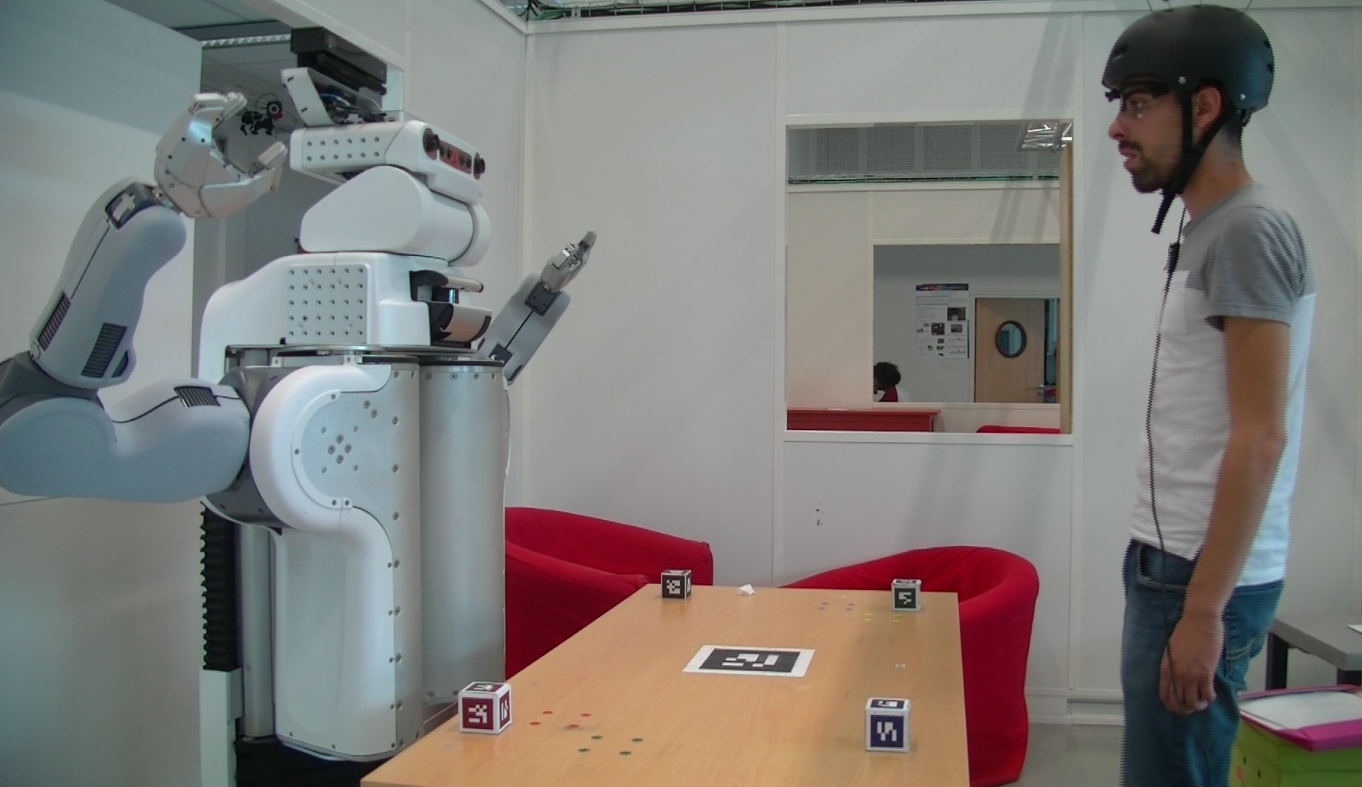
\includegraphics[width=0.45\textwidth]{figs/Chapter6/VideoInit.png}
       \label{subfig:videoInit}
   }
    %~
	\subfigure[End of the interaction. The stack should follow a precise order of colours (red, black, blue, green).]{
        \centering
        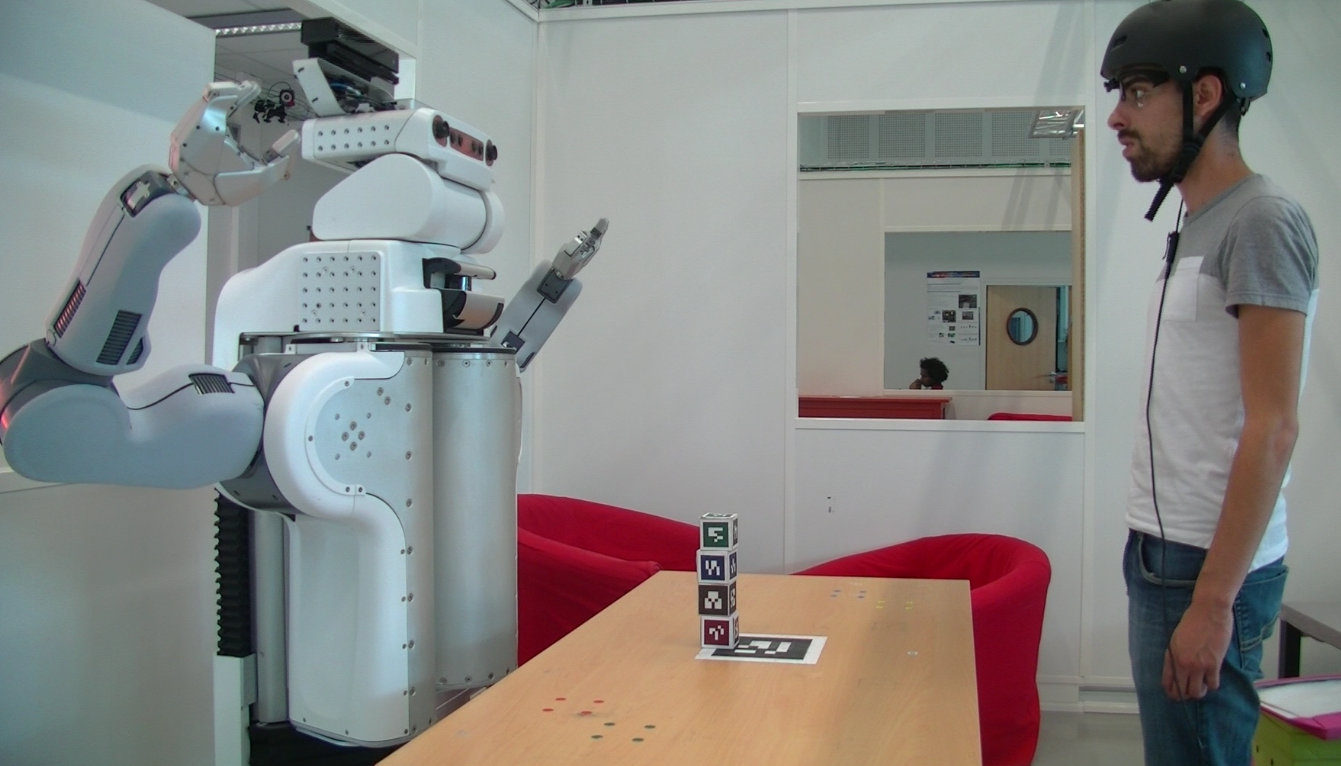
\includegraphics[width=0.45\textwidth]{figs/Chapter6/VideoGoal.png}
       \label{subfig:videoGoal}
   }
    \caption{Tasked used in the on-line video based study. In this task a human and a robot have to build a stack of coloured cubes. Different head behaviors of the robot was compared in the videos.}
    \label{fig:videoTask}
\end{figure*}

\subsection{Anticipation of robot actions}

The first behavior we studied concerns when the robot is performing actions. We asked ourself if the fact that the robot anticipates its next action with its head would benefit to the Joint Action and more particularly to the understanding of the robot actions by the human. To do so, we asked people to watch two videos: one with anticipation and one without. These two videos are focused on the first part of the interaction where the robot put the first two cubes on the stack. In the video without anticipation, the robot simply looks at the cube it is picking and the support where it is placing the cubes (as desribed in the "basic behavior"). In the video with anticipation the robot still looks at the cube it is picking and the supports where it is placing the cubes. However the robot starts looking the second cube to put on the stack while it is retracting from its first action (putting the first cube).

After having watched the two videos, participants were asked to answer several questions for each video. There was 4 5-scales questions for each video concerning the predictability of the robot behavior and the fact that the robot head behavior was adequate, clear and useful to the interaction. Then, the participants were asked to chose which video they preferred between the two videos (with the possibility to select both). These questions can be found in Appendix~\ref{chap:annexe2}. We also let a free space for comments at the end of the questionnaire.

The results of the questionnaire for this scenario can be found in Fig.~\ref{fig:resSce1}. No significant difference was found between the conditions either concerning the scores in the 5-scales questions (p=0.3467) or the preferences (p=0.3711). Indeed, based on the free comments of the participants, we found that they had difficulties to find the differences between both conditions, and, when they found the differences, they were sometime disturbed by the fact that the robot looks at an object without acting (in the condition with anticipation). 

We can conclude that the way we implemented anticipation is not conclusive for Joint Action, or at least for the kind of task tested here. Indeed, one factor here is that the task and needed actions are well known of both participant (as the stack order is predetermine, there is only one action to do at each time). Consequently, the anticipation may not be needed here but may be more interesting in a scenario where the human does not know the next robot action. Moreover, maybe the way the anticipation behavior is implemented is not the better way to do it. Further investigations may be needed on this subject.

\begin{figure*}[!h]
\centering
	\subfigure[Scores on the questions asked for each video of the scenario concerning the anticipation of robot actions. The score is the addition of the rates (in a scale of 5) of the 4 questions.]{
        \centering
        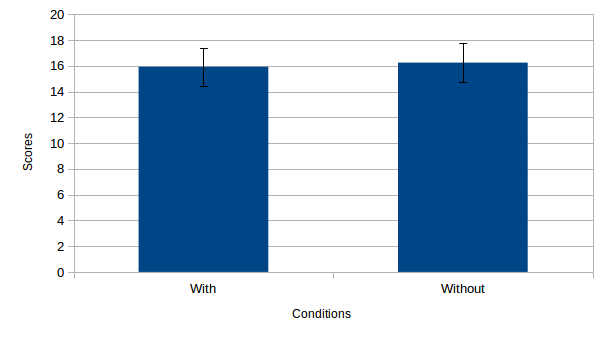
\includegraphics[width=0.45\textwidth]{figs/Chapter6/ScoresSce1.png}
       \label{subfig:scoresSce1}
   }
    %~
	\subfigure[Preferences for the scenario concerning the anticipation of robot actions. Numbers represent the number of times where a video was chosen for the preference question (on 59 participants).]{
        \centering
        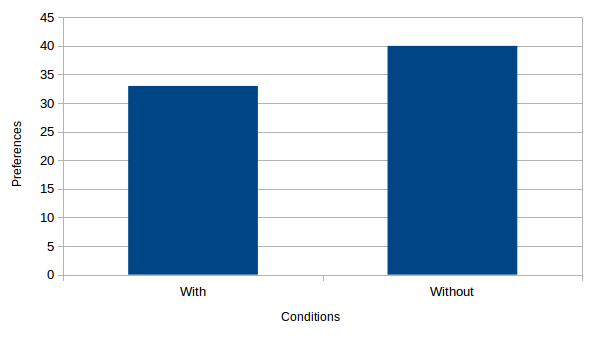
\includegraphics[width=0.45\textwidth]{figs/Chapter6/PrefSce1.png}
       \label{subfig:prefSce1}
   }
    \caption{Results for the scenario concerning the anticipation of robot actions. No significant differences was found between the two conditions (with anticipation and without anticipation).}
    \label{fig:resSce1}
\end{figure*}



\subsection{Following human's activity}

We then studied how the robot should show that it follows and understands human's actions. We want here to find a behavior adapted to the information the robot has concerning the human. In our system, the robot detects the human with a motion capture system (see description in Introduction) and has information about the head and the right hand positions and orientations. Here we tried to find a relatively simple behavior which, with a minimum of information allows the robot to show its attention and understanding. First, we compared different ways to decide when to look at the human's hand or when to look at the human's head. We compared three different conditions with videos based on the end of interaction (the part where the human puts the two last cubes). In all videos the human puts the two cubes one after the other. He also records a stop time during his first action by hesitating a short moment. In one condition, the robot looks at the human's hand whenever the hand is moving and looks at the human's head when the hand is not moving (with a small hysteresis in order to avoid going back and forth between the hand and the head). In the second condition, the robot looks at the human's hand whenever the hand is into a "working area" and at the human's head whenever the hand is not in the area. This "working area" is basically all the volume above the table. In the last condition, the robot looks at the human's hand whenever the hand is in the "working area" and is moving. Else the robot looks at the human head.

In the same way as for the previous scenario, participants were asked to answer several questions for each video. There was 4 5-scales questions for each video concerning the understanding of the human's actions by the robot and the fact that the robot head behavior was adequate, clear and useful to the interaction. Then, the participants were asked to choose which video they prefer between the three videos (with the possibility to select several). These questions can be found in Appendix~\ref{chap:annexe2}. We also let a free space for comments at the end of the questionnaire.

\begin{figure*}[!h]
\centering
	\subfigure[Scores on the questions asked for each video of the first scenario concerning the following of human's activity. The score is the addition of the rates (in a scale of 5) of the 4 questions.]{
        \centering
        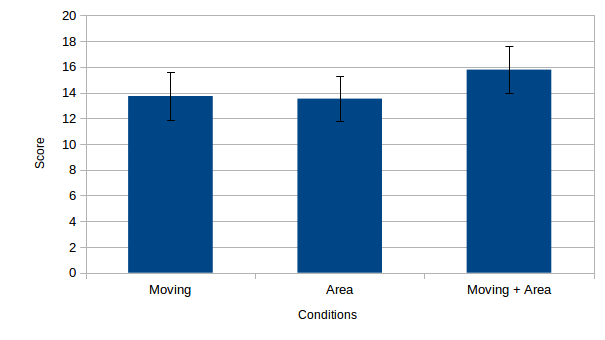
\includegraphics[width=0.45\textwidth]{figs/Chapter6/ScoresSce2.png}
       \label{subfig:scoresSce2}
   }
    %~
	\subfigure[Preferences for the first scenario concerning the following of human's activity. Numbers represent the number of times where a video was chosen for the preference question (on 59 participants).]{
        \centering
        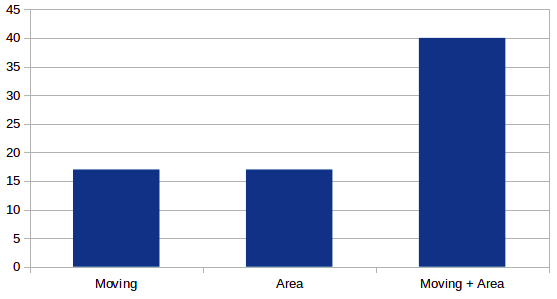
\includegraphics[width=0.45\textwidth]{figs/Chapter6/PrefSce2.png}
       \label{subfig:prefSce2}
   }
    \caption{Results for the the first scenario on the following of human's activity. The conditions where the robot looks at the human's hand whenever it is in a "working area " and moving has been significantly preferred to the two others.}
    \label{fig:resSce2}
\end{figure*}

The results of the questionnaire for this scenario can be found in Fig.~\ref{fig:resSce2}. The third condition (where the robot is considering area and movement) has been evaluated significantly higher than the two others (p < 0.01). No significant difference has been found between the two others videos. These results gives us leads for the construction of a robot head behavior. Indeed, we can see that with a minimal robot behavior (a simple switch between the hand and the head based on the hand position and movement), the robot is able to show its attention and understanding in a relatively acceptable way (rated at 15.78/20 in the 5-scale questions by the participant).

Then, we asked ourself if, when an action of the human is detected by the robot, the robot should show its understanding of the action by recording a small stop on the action. We asked participant to watch two videos. These video were also based on the end of interaction (the part where the human puts the two last cubes). In each video the human puts the two cubes one after the other and the robot was looking at human's hand and head following the third behavior described previously (where the robot considers area and movement). Additionally, in one video, the robot was making a stop on the stack each time the human placed a cube on it. The participants were asked to answer the same questions as for the previous scenario.

\begin{figure*}[!h]
\centering
	\subfigure[Scores on the questions asked for each video of the second scenario concerning the following of human's activity. The score is the addition of the rates (in a scale of 5) of the 4 questions.]{
        \centering
        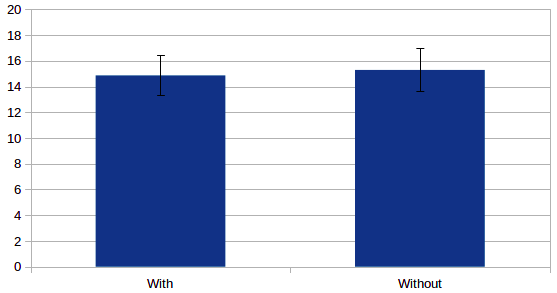
\includegraphics[width=0.45\textwidth]{figs/Chapter6/ScoresSce3.png}
       \label{subfig:scoresSce3}
   }
    %~
	\subfigure[Preferences for the second scenario concerning the following of human's activity. Numbers represent the number of times where a video was chosen for the preference question (on 59 participants).]{
        \centering
        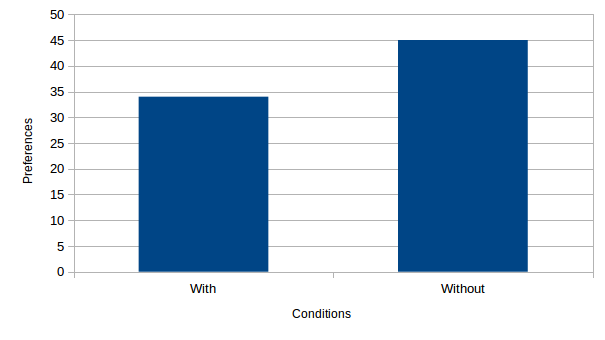
\includegraphics[width=0.45\textwidth]{figs/Chapter6/PrefSce3.png}
       \label{subfig:prefSce3}
   }
    \caption{Results for the second scenario on the following of human's activity. One condition includes a stop after each action of the human (With) while the other corresponds the the third behavior of the previous scenario (Without).}
    \label{fig:resSce3}
\end{figure*}

The results of the questionnaire for this scenario can be found in Fig.~\ref{fig:resSce3}. No significant difference was found between the conditions either concerning the scores in the 5-scales questions (p=0.33) or the preferences (p=0.1093). Indeed, based on the free comments of the participants, we found that they had difficulties to find the differences between both conditions, and, when they found the differences, they sometime disliked the fact that, when the robot makes a stop (in the condition with as stop), the robot does not follow anymore what the human is doing.


\subsection{Signalling human's actions}

Then, we bear interest to the signals the robot should give with its head concerning the Shared Plan execution. In this part, the videos were based on the middle of the interaction (the second cube of the robot and the first of the human).

The first signal we identified as potentially interesting concerns the signalling of an action the human should perform and is not performing. In all tested videos, the robot was putting its second cubes on the stack, then, the human was waiting a few moment before putting his cube. In one video, the robot was not giving any signal to the human, it was just following the "basic behavior" described earlier. In the two others videos, after a small waiting time, the robot gave a signal to the human for him to place his cube on the stack. In one video, the signal consisted on looking at the cube to take and then looking back at the human's head. In the other video, the signal consisted on looking at the cube, then looking at the stack and finally looking back at the human's head.

In the same way as for the previous scenarios, participants were asked to answer several questions for each video. There was 3 5-scales questions for each video which concerned the fact that the robot head behavior was adequate, clear and useful to the interaction. Then, the participants were asked to chose which video they prefer between the three videos (with the possibility to select several). These questions can be found in Appendix~\ref{chap:annexe2}. We also let a free space for comments at the end of the questionnaire.

\begin{figure*}[!h]
\centering
	\subfigure[Scores on the questions asked for each video of the first scenario concerning the signalling of human's actions. The score is the addition of the rates (in a scale of 5) of the 3 questions.]{
        \centering
        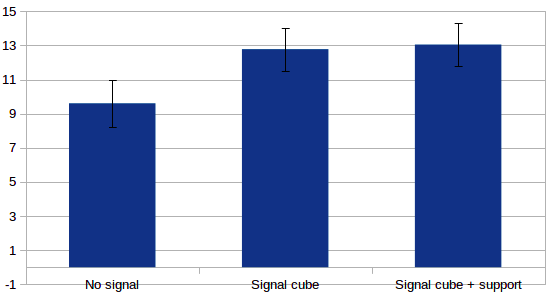
\includegraphics[width=0.45\textwidth]{figs/Chapter6/ScoresSce4.png}
       \label{subfig:scoresSce4}
   }
    %~
	\subfigure[Preferences for the first scenario concerning the signalling of human's actions. Numbers represent the number of times where a video was chosen for the preference question (on 59 participants).]{
        \centering
        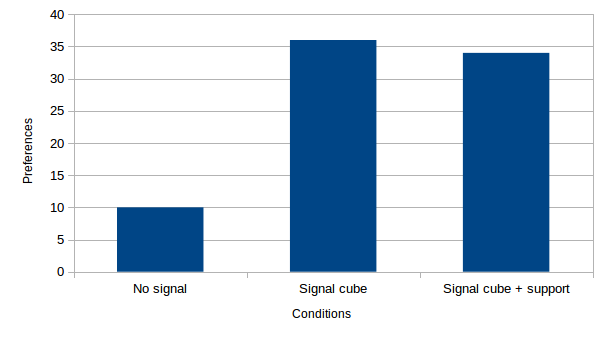
\includegraphics[width=0.45\textwidth]{figs/Chapter6/PrefSce4.png}
       \label{subfig:prefSce4}
   }
    \caption{Results for the first scenario on the signalling of human's actions. In one condition the robot was not giving any signal to the human (No signal). In another conditions the robot was giving a signal consisting of looking at the cube to place and looking back at the human's head (Signal cube). In the last condition the robot was giving a signal consisting of looking at the cube to place, the stack and then looking back at the human's head (Signal cube + stack).}
    \label{fig:resSce4}
\end{figure*}

The results of the questionnaire for this scenario can be found in Fig.~\ref{fig:resSce4}. The first condition (where there is no signal) has been evaluated significantly lower than the two others (p < 0.01). No significant difference has been found between the two different signals given by the robot. These results show us that the studied signal (the robot signals to the human that he should act when he is not acting) is considered important by peoples. One possible explanation concerning the lack of difference between the two ways tested to perform the signal is that, in this task, there is only one place where to put the cube. Indeed, in the signal where the robot looks at the stack, the information given is not so interesting in this configuration. Further investigations can be interesting with scenarios where the human has several choices of actions to execute.

Then, we investigated the use of a signal to help turn-taking. We specifically focused on the signal needed at the end of a robot action if the next action to be performed is a human action. In this scenario, we compared 4 videos where the robot puts its second cube and then the human puts his first cube. In two videos the robot was giving a signal to the human at the end of its action. This signal consisted in looking at the human's head, looking at the cube he should put on the stack and then looking back at the human's head. In one of these two videos, the robot was giving the signal while retracting from its action. In the other the robot was giving the signal after retracting from its action. In the two other videos, the robot was not giving signal to the human. In one case its looks at the human's head as soon as its over its action (while retracting), in the other case it looks at the human's head only after retracting from its action. The participants were asked to answer the same questions as for the previous scenario.

\begin{figure*}[!h]
\centering
	\subfigure[Scores on the questions asked for each video of the second scenario concerning the signalling of human's actions. The score is the addition of the rates (in a scale of 5) of the 3 questions.]{
        \centering
        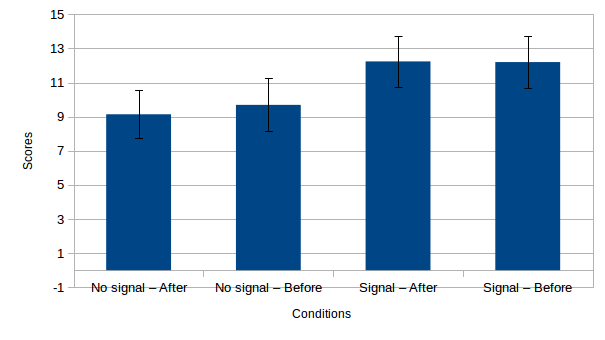
\includegraphics[width=0.45\textwidth]{figs/Chapter6/ScoresSce5.png}
       \label{subfig:scoresSce5}
   }
    %~
	\subfigure[Preferences for the second scenario concerning the signalling of human's actions. Numbers represent the number of times where a video was chosen for the preference question (on 59 participants).]{
        \centering
        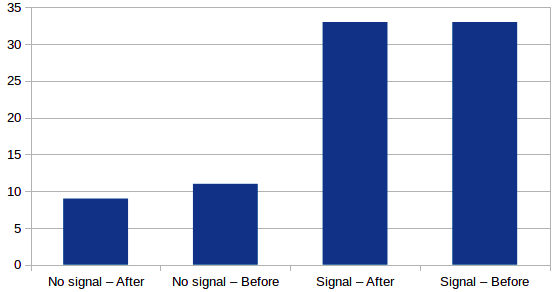
\includegraphics[width=0.45\textwidth]{figs/Chapter6/PrefSce5.png}
       \label{subfig:prefSce5}
   }
    \caption{Results for the second scenario on the signalling of human's actions. In one condition the robot was not giving any signal to the human and was looking at his head after retracting (No signal - After). In another condition, the robot was not giving any signal to the human and was looking at his head while retracting (No signal - Before). In the two others conditions the robot was giving a signal consisting in looking at the the human's head, looking at the cube to place on the stack and looking back at the human's head. In one condition the robot was giving the signal after retracting from its action (Signal - After) and in the other while retracting (Signal - Before).}
    \label{fig:resSce5}
\end{figure*}

The results of the questionnaire for this scenario can be found in Fig.~\ref{fig:resSce5}. The two conditions where there is a signal have been evaluated significantly higher than the two others (p < 0.01). No significant difference has been found between the two conditions whit a signal as well as for the two conditions without a signal. These results show the usefulness of a signal at the end of robot actions in order to help turn-taking. However, apparently the timing of the signal (during or after retracting) has not been found important by the users. 

\subsection{Finding the priority target}

In the last scenario of the study, we focused on the decision to take when the robot has several possible target to look. We studied here the case where the robot is executing an action (and so have a target for its action) and the human performs another action at the same time (and so the robot should also look at the human's action). In the videos, the robot is still placing its second cube on the stack when the human picks his next cube (in prevision of placing it on the stack). In each video, the robot looks at the stack when putting its cube. In one video, the robot does not look at all at the human action. In another video, the robot looks at the human action (it looks at the human's hand and goes back to the stack) when it is executed without interrupting its action. In the last video, the robot stops its action to look at the human action and then restarts its action.

In the same way as for the previous scenarios, participants were asked to answer several questions for each video. There was 3 5-scales questions for each video concerning the fact that the robot behavior was adequate, clear and useful to the interaction. Then, the participants were asked to chose which video they prefer between the three videos (with the possibility to select several). These questions can be found in Appendix~\ref{chap:annexe2}. We also let a free space for comments at the end of the questionnaire.

\begin{figure*}[!h]
\centering
	\subfigure[Scores on the questions asked for each video of the scenario concerning the priority target. The score is the addition of the rates (in a scale of 5) of the 3 questions.]{
        \centering
        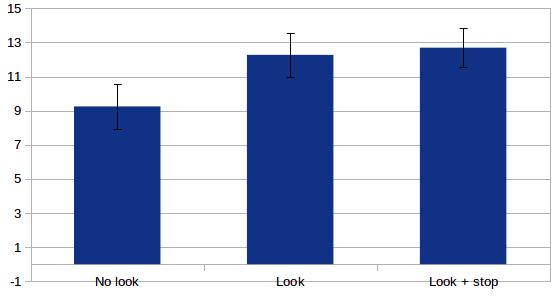
\includegraphics[width=0.45\textwidth]{figs/Chapter6/ScoresSce6.png}
       \label{subfig:scoresSce6}
   }
    %~
	\subfigure[Preferences for the first scenario concerning the scenario concerning the priority target. Numbers represent the number of times where a video was chosen for the preference question (on 59 participants).]{
        \centering
        \includegraphics[width=0.45\textwidth]{figs/Chapter6/PrefSce6.png}
       \label{subfig:prefSce6}
   }
    \caption{Results for the scenario concerning the priority target. In one condition the robot was not looking at the human's action (No look). In another conditions the robot was looking at the human's action without interrupting its action (Look). In the last condition the robot was interrupting its action to look at the human's action (Look + stop).}
    \label{fig:resSce6}
\end{figure*}

The results of the questionnaire for this scenario can be found in Fig.~\ref{fig:resSce6}. The condition where the robot does not look at the human's action has been evaluated significantly lower than the two others (p < 0.01). No significant difference has been found between the two conditions where the robot looks at the human's action. These results show us that even if the robot is busy to something else it is important that it looks at human's action to acknowledge the fact that it perceived the action. If the robot action requires the full focus of the robot head, the robot can interrupt briefly its action in order to look at the human's action without degrading the acceptability of its behavior.


\section{The robot head behavior}

Based on our previous analysis and the performed on-line user study we start conceiving an architecture to generate a robot head behavior. This behavior is for now computed based on a Joint Action with only one human.

The architecture can be found in Fig.~\ref{fig:headArchi}. We can find in this architecture the four "families" described in Sec.~\ref{sec:reflection} (human observation, robot action, dialogue and coordination). Based on informations concerning humans, the robot constantly computes a target (either an object or a part of the human body) to look. In addition, when the robot is performing an action, it also computes a target for the action. In a same way, when the robot is conversing with a human, another target is computed. Based on the current state of the Shared Plan, the robot also computes signals to give to the human. Finally, based on the different targets and signals, an arbitration module chooses at each time the final target to look.

\begin{figure}[!h]
	\centering
    \includegraphics[width=0.9\textwidth]{figs/Chapter6/Head_archi.png}
    \caption{The architecture to generate the robot head behavior. The arbitration modules chooses where the robot should look based on several possible behaviors and signals. The possible behaviors concern the human activity, the current robot action and the current state of the dialogue. Coordination signals are computed based on the current Shared Plan.}
    \label{fig:headArchi}
\end{figure}

In this architecture, a target is described as a point to look (either an object or a part of the human body) and an associated priority.
$$target = <point, priority>$$
A signal is described as a ordered set of points to look with associated durations, a priority, an expiration time and possibles expiration conditions (events).
$$signal = <points, durations, priority, expiration_time, expiration_conditions>$$

This architecture is still work in progress, there is still needs of deepening for some parts and the parametrisation of the priorities and durations are still needed.

\subsection{Observation target}

We saw previously that the robot should show its interest and understanding of the human activity. We studied in the previous section how we can show the interest of the robot in the human's actions based on the position and movements of his hand. We keep the condition of the study which was the highest marks: the robot looks at the human's hand whenever the hand is moving (with a small hysteresis in order to avoid going back and forth between the hand and the head) and into a "working area". Working areas can be defined dynamically and attached to objects (e.g. everything above a table).

Additionally to this behavior, another important feature is joint attention. When the human stares at another for a sufficient time, the robot should also look at this object. In a same way, if the human stares at the robot, the robot should turn back his look. The given algorithm to compute the point corresponding to the human observation can be found in Alg.~\ref{alg:observation}.


\begin{algorithm}
\caption{Computation of the point to look based on human's activity}
\label{alg:observation}
\begin{algorithmic}
\REQUIRE human's hand position and movement, objects position, human's  head position and target
\IF {human's head target = robot > t}
\STATE $point = human's \ head$\hfill \textit{$\vartriangleright$ the human stares at the robot}
\ELSIF{human's head target = object > t}
\STATE $point = object$\hfill \textit{$\vartriangleright$ the human stares at an object}
\ELSIF{human's hand is moving $\&$ human's hand is in "working area"}
\STATE $point = human's \ hand$\hfill \textit{$\vartriangleright$ following human's action}
\ELSE
\STATE $point = human's \ head$\hfill \textit{$\vartriangleright$ by default, looking at human's head}
\ENDIF
\RETURN $point$
\end{algorithmic}
\end{algorithm}

This behavior is for now really basic. One the reason is that we want a behavior which can work with few information concerning the human (here only concerning the head and one hand). Moreover, we strongly think, even if it remains to be proofed, that a minimal behavior is sometime preferred as a more complex one as soon as all the needed components are here.

\subsection{Robot action and dialogue targets}

We saw the importance of having a head behavior in adequacy with the robot current action. Consequently, the action target is computed directly by the component in charge of executing robot actions and depends of the action executed. The point to look is in major cases the "target" object (e.g. the object to pick or the support where to place). The priority associated with this point principally depends of the fact that the action requires the head focus (e.g. at the beginning of a pick action, the priority will be higher to unsure the good perception of the object). The module in charge of executing actions has also access to the point the robot is looking in order to adapt the action execution (e.g suspend if necessary).

In a same way, the target associated to dialogue is directly computed by the module in charge of the dialogue. It mainly consists in looking at the human when talking and at the objects the robot is referring to.

\subsection{Coordination signals}

We saw the importance of coordination signals during Joint Action execution. In this work, these signals are based on the execution of the Shared Plan. The first two signals are the one studied in the on-line study. The first one is computed whenever a human has an action to execute and is not performing it after a certain amount of time (and that he is not doing another action). In this case, the robot signals to the human the action he should execute. This signal consist of looking at the human's head, then the different points of interest of the action to execute and finally looking at the human's head again. The points of interest of an action are ordered and defined for each high level action (e.g. for the pick and place action it is the object to pick and, then, the support where to place). This signal should have a relatively long expiration precise time as its timing is not crucial. It should also have the execution of the awaited action in its expiration conditions.

Another signal concerns the help of turn-taking. After each robot action, if this action unlocks another action attributed to the human (there is a causal link between the two actions), the robot sends a signal to the human to execute the action. This signal consists of looking at the human's head, then the different points of interest of the action to execute and finally looking at the human's head again. This signal should have a small expiration time as it has to be performed just after the robot action. It should also have the execution of the awaited action in its expiration conditions.

Finally, we saw the importance of looking at a human's actions, even if the robot is currently busy to something else. To do so, when the human performs an action, a signal is computed with a high priority as well as a small expiration time because the signal does not make sense if it comes latter after the action. This signal consists of looking a the point of interest of the executed action. 

\subsection{Arbitration}

The arbitration of the the different points to look and the different signals to give is based on priorities. The arbitration module first chooses the point to look with the higher priority between the ones from human observation, dialogue and robot action. Then, when a signal is send by the coordination module, it is stored in a waiting list (ordered by priorities). If the priority of a signal in the waiting list is higher than the current priority of the chosen point to look, the robot executes the signal. In order to keep signals consistencies, a signal started can not be interrupted even if there is another priority signal or point to look. When a signal expires (the expiration time is reached or an expiration condition is true) the signal is removed from the waiting list.

They may be some missing signals in the current version of the architecture. However, we strongly think that it has been think in a sufficiency generic way in order to integrate new signals if needed.

\section{Conclusion}

In this chapter, we studied non-verbal behavior during human-robot Joint Action, and more especially the robot head behavior. A first bibliographic study has been done in order to identify the needed components of a robot head behavior adapted to the Joint Action. Then, some specific parts of these components have been studied with an on-line video based study. Finally, an architecture to generate the robot head behavior has been proposed. This architecture, still in construction, should allow the robot to produce a head behavior which provides the needed information in order for the robot to show its attention, make its action understandable, dialogue and coordinate the  Joint Activity based on the Shared Plan. They may be some missing signals or behavior in the current version of the architecture. However, we strongly think that it has been think in a sufficiency generic way in order to easily integrate them to the architecture. 

\ifdefined\included
\else
\bibliographystyle{StyleThese}
\bibliography{These}
\end{document}
\fi

\ifdefined\included
\else
\documentclass[english,a4paper,11pt,twoside]{StyleThese}
\usepackage{amsmath,amssymb}             % AMS Math
\usepackage[T1]{fontenc}
\usepackage[utf8x]{inputenc}
\usepackage{babel}
\usepackage{datetime}

\usepackage{lmodern}
\usepackage{tabularx}
%\usepackage{tabular}
\usepackage{multirow}

\usepackage{subfigure}
\usepackage{fancyvrb}
\usepackage{algorithmic}
\usepackage{algorithm}
\usepackage{mathtools}


\usepackage{hhline}
\usepackage[left=1.5in,right=1.3in,top=1.1in,bottom=1.1in,includefoot,includehead,headheight=13.6pt]{geometry}
\renewcommand{\baselinestretch}{1.05}

% Table of contents for each chapter

\usepackage[nottoc, notlof, notlot]{tocbibind}
\usepackage{minitoc}
\setcounter{minitocdepth}{2}
\mtcindent=15pt
% Use \minitoc where to put a table of contents

\usepackage{aecompl}


% Glossary / list of abbreviations

\usepackage[intoc]{nomencl}
\iftoggle{ThesisInEnglish}{%
\renewcommand{\nomname}{Glossary}
}{ %
\renewcommand{\nomname}{Liste des Abréviations}
}

\newcommand{\accom}[1]{\textcolor{red}{[#1]}}

\makenomenclature

% My pdf code

\usepackage{ifpdf}

\ifpdf
  \usepackage[pdftex]{graphicx}
  \DeclareGraphicsExtensions{.jpg}
  \usepackage[a4paper,pagebackref,hyperindex=true]{hyperref}
  \usepackage{tikz}
  \usetikzlibrary{arrows,shapes,calc}
\else
  \usepackage{graphicx}
  \DeclareGraphicsExtensions{.ps,.eps}
  \usepackage[a4paper,dvipdfm,pagebackref,hyperindex=true]{hyperref}
\fi

\graphicspath{{.}{images/}}

%% nicer backref links. NOTE: The flag ThesisInEnglish is used to define the
% language in the back references. Read more about it in These.tex

\iftoggle{ThesisInEnglish}{%
\renewcommand*{\backref}[1]{}
\renewcommand*{\backrefalt}[4]{%
\ifcase #1 %
(Not cited.)%
\or
(Cited in page~#2.)%
\else
(Cited in pages~#2.)%
\fi}
\renewcommand*{\backrefsep}{, }
\renewcommand*{\backreftwosep}{ and~}
\renewcommand*{\backreflastsep}{ and~}
}{%
\renewcommand*{\backref}[1]{}
\renewcommand*{\backrefalt}[4]{%
\ifcase #1 %
(Non cité.)%
\or
(Cité en page~#2.)%
\else
(Cité en pages~#2.)%
\fi}
\renewcommand*{\backrefsep}{, }
\renewcommand*{\backreftwosep}{ et~}
\renewcommand*{\backreflastsep}{ et~}
}

% Links in pdf
\usepackage{color}
\definecolor{linkcol}{rgb}{0,0,0.4} 
\definecolor{citecol}{rgb}{0.5,0,0} 
\definecolor{linkcol}{rgb}{0,0,0} 
\definecolor{citecol}{rgb}{0,0,0}
% Change this to change the informations included in the pdf file

\hypersetup
{
bookmarksopen=true,
pdftitle="Joint Action for Human-Robot Interaction",
pdfauthor="Sandra DEVIN", %auteur du document
pdfsubject="Thesis", %sujet du document
%pdftoolbar=false, %barre d'outils non visible
pdfmenubar=true, %barre de menu visible
pdfhighlight=/O, %effet d'un clic sur un lien hypertexte
colorlinks=true, %couleurs sur les liens hypertextes
pdfpagemode=None, %aucun mode de page
pdfpagelayout=SinglePage, %ouverture en simple page
pdffitwindow=true, %pages ouvertes entierement dans toute la fenetre
linkcolor=linkcol, %couleur des liens hypertextes internes
citecolor=citecol, %couleur des liens pour les citations
urlcolor=linkcol %couleur des liens pour les url
}

% definitions.
% -------------------

\setcounter{secnumdepth}{3}
\setcounter{tocdepth}{2}

% Some useful commands and shortcut for maths:  partial derivative and stuff

\newcommand{\pd}[2]{\frac{\partial #1}{\partial #2}}
\def\abs{\operatorname{abs}}
\def\argmax{\operatornamewithlimits{arg\,max}}
\def\argmin{\operatornamewithlimits{arg\,min}}
\def\diag{\operatorname{Diag}}
\newcommand{\eqRef}[1]{(\ref{#1})}

\usepackage{rotating}                    % Sideways of figures & tables
%\usepackage{bibunits}
%\usepackage[sectionbib]{chapterbib}          % Cross-reference package (Natural BiB)
%\usepackage{natbib}                  % Put References at the end of each chapter
                                         % Do not put 'sectionbib' option here.
                                         % Sectionbib option in 'natbib' will do.
\usepackage{fancyhdr}                    % Fancy Header and Footer

% \usepackage{txfonts}                     % Public Times New Roman text & math font
  
%%% Fancy Header %%%%%%%%%%%%%%%%%%%%%%%%%%%%%%%%%%%%%%%%%%%%%%%%%%%%%%%%%%%%%%%%%%
% Fancy Header Style Options

\pagestyle{fancy}                       % Sets fancy header and footer
\fancyfoot{}                            % Delete current footer settings

%\renewcommand{\chaptermark}[1]{         % Lower Case Chapter marker style
%  \markboth{\chaptername\ \thechapter.\ #1}}{}} %

%\renewcommand{\sectionmark}[1]{         % Lower case Section marker style
%  \markright{\thesection.\ #1}}         %

\fancyhead[LE,RO]{\bfseries\thepage}    % Page number (boldface) in left on even
% pages and right on odd pages
\fancyhead[RE]{\bfseries\nouppercase{\leftmark}}      % Chapter in the right on even pages
\fancyhead[LO]{\bfseries\nouppercase{\rightmark}}     % Section in the left on odd pages

\let\headruleORIG\headrule
\renewcommand{\headrule}{\color{black} \headruleORIG}
\renewcommand{\headrulewidth}{1.0pt}
\usepackage{colortbl}
\arrayrulecolor{black}

\fancypagestyle{plain}{
  \fancyhead{}
  \fancyfoot{}
  \renewcommand{\headrulewidth}{0pt}
}

%\usepackage{MyAlgorithm}
%\usepackage[noend]{MyAlgorithmic}
\usepackage[ED=MITT - STICIA, Ets=INP]{tlsflyleaf}
%%% Clear Header %%%%%%%%%%%%%%%%%%%%%%%%%%%%%%%%%%%%%%%%%%%%%%%%%%%%%%%%%%%%%%%%%%
% Clear Header Style on the Last Empty Odd pages
\makeatletter

\def\cleardoublepage{\clearpage\if@twoside \ifodd\c@page\else%
  \hbox{}%
  \thispagestyle{empty}%              % Empty header styles
  \newpage%
  \if@twocolumn\hbox{}\newpage\fi\fi\fi}

\makeatother
 
%%%%%%%%%%%%%%%%%%%%%%%%%%%%%%%%%%%%%%%%%%%%%%%%%%%%%%%%%%%%%%%%%%%%%%%%%%%%%%% 
% Prints your review date and 'Draft Version' (From Josullvn, CS, CMU)
\newcommand{\reviewtimetoday}[2]{\special{!userdict begin
    /bop-hook{gsave 20 710 translate 45 rotate 0.8 setgray
      /Times-Roman findfont 12 scalefont setfont 0 0   moveto (#1) show
      0 -12 moveto (#2) show grestore}def end}}
% You can turn on or off this option.
% \reviewtimetoday{\today}{Draft Version}
%%%%%%%%%%%%%%%%%%%%%%%%%%%%%%%%%%%%%%%%%%%%%%%%%%%%%%%%%%%%%%%%%%%%%%%%%%%%%%% 

\newenvironment{maxime}[1]
{
\vspace*{0cm}
\hfill
\begin{minipage}{0.5\textwidth}%
%\rule[0.5ex]{\textwidth}{0.1mm}\\%
\hrulefill $\:$ {\bf #1}\\
%\vspace*{-0.25cm}
\it 
}%
{%

\hrulefill
\vspace*{0.5cm}%
\end{minipage}
}

\let\minitocORIG\minitoc
\renewcommand{\minitoc}{\minitocORIG \vspace{1.5em}}

\usepackage{multirow}
%\usepackage{slashbox}

\newenvironment{bulletList}%
{ \begin{list}%
	{$\bullet$}%
	{\setlength{\labelwidth}{25pt}%
	 \setlength{\leftmargin}{30pt}%
	 \setlength{\itemsep}{\parsep}}}%
{ \end{list} }

\newtheorem{definition}{Définition}
\renewcommand{\epsilon}{\varepsilon}

% centered page environment

\newenvironment{vcenterpage}
{\newpage\vspace*{\fill}\thispagestyle{empty}\renewcommand{\headrulewidth}{0pt}}
{\vspace*{\fill}}

\usepackage{tablefootnote}

\sloppy
\begin{document}
\setcounter{chapter}{6} %% Numéro du chapitre précédent ;)
\dominitoc
\faketableofcontents
\fi

\chapter{Combining learning and planning}
\minitoc

\section{Motivation}

When it comes to decisional process in robotics, two main schools of though can be distinguished: machine learning and deterministic processes such as planing or states machines. Both ways have their advantages and disadvantages. Learning is usually "cheap" (the decision process is quick) and always proposes a solution to a given problem. However, learning requires either a big amount of data or a long period of learning. Moreover, during the learning period, the robot can produce inconsistent behavior which can be confusing for a potential human collaborator. On the other hand, planing can take into account humans through social rules and ensure the validity of a whole solution. However, planing does not learn from human behavior, and, when it comes to complex tasks or environments, it can become slow to propose a solution. The idea of this work is to propose a solution where we combine planing and learning in the context of human-robot interaction in order to take advantage of both. 

This work has been done in collaboration with ISIR at Paris and more particularly with another PhD student Erwan Renaudo. It has been done in the context of the RoboErgoSum ANR project\footnote{http://roboergosum.isir.upmc.fr/}. This work is based on the work of \cite{renaudo2014design} and has been the subject of a publication in a workshop at the RoMan conference \cite{renaudo2015learning} as well as a part of a journal article \cite{khamassi2016integration}.

\section{Background}

\subsection{Inspiration from neurosciences}

Seminal works on living being behaviors have been done in the late 19th century - beginning of the 20th century - with experiments on mammals. One pioneer work concerning the learning process is the experiment of the cat in a box \cite{thorndike1998animal}. In this experiment, a cat is put in a box each time it is hungry. The cat can see food outside of the box and a system of lever allows it to open the box. Each time the cat is put in the box it takes less time to go out. This experiment allows to show the principle of learning through trial and error. 

Latter, studies have highlighted two main kinds of behavior during decision-making tasks. \textbf{Goal-directed behaviors} are governed by estimates of action-outcome contingencies (i.e. decision-making relies on the prior estimation of the outcome expected after an action or an action sequence) and are mainly active at the beginning of the task. Then, when the animal is well trained in the task under stable conditions, a transfer of control to \textbf{habitual behaviors} governed by stimulus-response associations occurs  \cite{dickinson1985actions}. When rodents, monkeys or humans start a new decision-making task, they appear to initially rely on their goal-directed system. They take time to analyse the structure of the task in order to build an internal model of it, and make slow decisions by planning and inferring the long-term consequences of their possible actions before deciding what to do next. Then as their performance gradually improve, they appear to make quicker and quicker decisions, relying on their habitual system which slowly acquires simple stimulus-response associations to solve the task. Finally, when subjects restart to make errors after a task change, they appear to restart planning within their internal model and thus slow down their decision process before acquiring the new task contingencies \cite{balleine2010human, dolan2013goals}. The coordination of these two learning systems allows mammals to avoid long and costly computations when the environment is sufficiently stable, while still enabling animals to detect environmental changes requiring to update their internal model and replan.

In computational neuroscience models, these behaviors are modeled using the theory of Reinforcement Learning \cite{sutton1998introduction}: model-based and model-free algorithms provide a direct analogy with goal-directed and habitual behaviors \cite{daw2005uncertainty}. More recently, different computational criteria have been proposed to decide when to shift between model-based and model-free experts \cite{pezzulo2013mixed, lesaint2014modelling, viejo2015modeling}. Applied to neuroscience tasks, the work from \cite{daw2005uncertainty} proposes that the most certain expert gets control on the agent, while \cite{keramati2011speed} balance speed and accuracy using the cost of planning versus the gain of information. A third approach proposes, in the context of navigation strategies, that a coordination module learns by reinforcement the most efficient behavior (in terms of average obtained reward) in each state \cite{dolle2010path}.

\subsection{Learning in human-robot interaction}

A major part of robotics decision-making algorithms are based on planning processes which take into account a great number of information (\cite{ingrand2014deliberation}). These approaches to decision-making could be seen as similar to what neuroscientists call the goal-directed system, except that there is most of the time no learning in the system. Such approaches have been extended to HRI by taking into account human-aware costs such as social-rules and humans comfort and preferences \cite{cirillo2010human,Lallement2014hatp}.

Besides, robots learning abilities are still very limited and require the injection of important prior knowledge by the human in the robot’s decision-making system. Early applications of reinforcement learning (RL) algorithms to robotics \cite{hayes1994robot, morimoto2001acquisition, smart2002effective} - some of which being neuro-inspired - produced limited progresses, due to applications to relatively simple problems (with a small number of states and actions), to slowness in learning and to systematic instability observed throughout the learning process. More recent applications of RL to robotics have permitted to deal with more complex and continuous action spaces, enabling to learn efficient sensorimotor primitives \cite{kober2011learning, martins2010learning, stulp2013robot}. These approaches have been extended in HRI to allow robots to learn to collaborate with humans.
In several works, the reward signal is interactively assigned by the human \cite{kaplan2002robotic, knox2012reinforcement} while other works use the human to provide demonstrations to the robot \cite{nicolescu2003natural, thomaz2006reinforcement}.
A method of cross-training is used and compared to standard reinforcement learning algorithms in the context of human-robot teamwork in \cite{nikolaidis2013human}. Cross-training is an interactive planning method in which a human and a robot iteratively switch roles to learn a shared plan for a collaborative task. Such approaches to decision-making could be seen as similar to what neuroscientists call habitual behaviors.

Even if we can find more and more interesting works in HRI concerning planing and learning for the robot to collaborate with humans, there is no work to our knowledge concerning how to combine both approaches into a robotics architecture.

\section{Experts presentation}

Inspired from from neuroscience theories and based on the previous work of \cite{renaudo2014design} the aim of this work is to combine goal-directed and habitual behaviors in the context of human-robot Joint Action. To do so, we use two experts which implement these two kinds of behavior. The goal-directed behavior is produced here by HATP (Human-Aware Task Planer), a task planner which has proved its efficiency in the field of human-robot interaction. A Qlearning algorithm allows to implement the habitual behavior. We will describe in this section these two experts and their respective strengths and weakness. The next sections will show how we combined those two experts into two different architectures.

\subsection{HATP}

In our work, the goal-directed behavior is provided by HATP, an HTN (Hierarchical Task Network, \cite{erol1994htn}) task planner which has been conceived to work in the context of human-robot collaboration.  As a HTN planner, HATP uses known preconditions and effects of actions in order to find the best plan that reaches the given goal. It takes as input a list of all possible actions and their description in terms of preconditions and effects and also a description of the current world state as a set of predicates. Then, it looks for the combination of actions that minimizes the solution cost. This cost is computed based on execution time and human-aware costs (e.g the balance of efforts between agents or the waiting time of the human partner). This plan is meant to be executed step by step until the goal is reached. An example of such a plan can be found Fig.~\ref{fig:examplePlan}.

\begin{figure}[!h]
	\centering
    \includegraphics[width=0.9\textwidth]{figs/Chapter7/SharedPlan.png}
    \caption{An example of a Shared Plan computed by HATP. This plan allows a human and a robot to build a stack of colored objects together by placing them one on-top of the others.}
    \label{fig:examplePlan}
\end{figure}

\subsection{Qlearning algorithm (MF)}

The habitual behavior is provided by a model-free reinforcement learning algorithm (MF) that directly learns the state–action associations by caching in each state the earned rewards in the value of each action. In this implementation, the algorithm is implemented as a neural network (see Fig.~\ref{fig:Qlearning}). The network input neurons represent the different possible states and the output neurons encode the estimation of action values in the current state. The weights are modified to associate each state with the most rewarding action in the current task.

A method similar to \cite{brafman2002r} is used to compute the value $Qt(St, a_j)$ of an action $a_j$ in a certain state $S$. $Qt(St, a_j)$ is represented as the scalar product between the input vector and the weights $W_j = (w_{0j} , . . . , w_{Nj})$ linking to this action:
$$Qt(St, a_j) = W_j^t \ . \ (S_t, 1)$$

here we set weights at a positive value to provide an initial optimistic estimate of action values ($w_0$ = 0.5). Weights $W_t$ are updated according to the Qlearning algorithm \cite{watkins1989learning}. The Reward Prediction Error $\delta$ is spread over the weights of the previously active input and the action $a$ done in the corresponding state:
$$\delta = r_t + \gamma_{Hab} \ . \ \underset{b \in A}{max}(W_b^{t-1}) \ . \ S_t - (W_a^{t-1} \ . \ S_{t-1})$$
$$W_a^t = W_a^{t-1} + \alpha_{Hab} \ . \ \delta / \underset{n}{\Sigma}s_{n}$$

with $r_t$ the instant reward received for performing a in $S_{t−1}$ , $\alpha_{Hab}$ the learning rate, $\gamma_{Hab}$ the decay rate of future rewards. The weights are updated locally: only the state from which the action has been performed is updated. Thus, it requires for the agent to visit every known state of the problem to update values.


\begin{figure}[!h]
	\centering
    \includegraphics[width=0.6\textwidth]{figs/Chapter7/Qlearning.png}
    \caption{Habitual expert, modeled as a Qlearning algorithm implemented as a neural network. The expert receives a state $S$ which is projected onto the input neurons $s_i$, defining an input activity. This activity is propagated through the network weights $W$ to generate activity of the action layer. This activity corresponds to the values $Q(S, a_j)$, with each neuron coding for a distinct action. This value distribution is converted in probability distribution using a softmax function, which allows the expert to make a decision $D$ on the next action to perform.}
    \label{fig:Qlearning}
\end{figure}

\subsection{Experts comparison}

The two different experts have really different ways to decide of the next action to execute. Both methods have their advantages and disadvantages:
\begin{itemize}
\item HATP looks for a complete solution to achieve the given goal while the MF only looks for the next action which maximize the probability to get a reward. Consequently, HATP ensures the feasibility of the solution proposed but could find itself in a state where it does not find a valid solution and so where it will not be able to propose an action. In the other hand, the MF does not ensure that its proposed action allows to achieve the goal but will always propose an action to perform.
\item As HATP computes a whole plan to achieve the goal, its cost, in the sense of time to take a decision, is far bigger than the one of the MF which only proposes the next action. However, this difference needs to be weighed by the fact that as an HATP plan is composed of several actions, this cost is not needed at each step of the task. Moreover, this cost stay acceptable in a not so complex task.
\item HATP is conceived to produce a robot behavior understandable and acceptable by the human. The actions it proposes will produce a consistent behavior of the robot with which one the human can easily collaborate. For its part, the MF has a long period of learning during which one the behavior produced is inconsistent and can be really disturbing for a human collaborating with the robot. Moreover, each time a change happens in the task, a new learning phase is needed. However, the MF is able to learn to adapt its behavior to the human whereas the HATP policy is defined off-line and can not be updated with the behavior of the human during the interaction.
\end{itemize}


\section{First architecture: a proof of concept}


\subsection{Control architecture}


\begin{figure}[!h]
	\centering
    \includegraphics[width=0.8\textwidth]{figs/Chapter7/FirstArchi.png}
    \caption{First tried architecture to combine the two experts. The Situation Assessment module gets data from perception and maintains the current world state. This world state is used by the supervision to compute the reward and by the experts to take decisions. The propositions of the two experts are sent to the meta controller which decides of the action to execute. The supervisor executes the action with the help of lower execution modules.}
    \label{fig:FirstArchi}
\end{figure}

The first architecture we tried to combine the two experts is the one Fig.~\ref{fig:FirstArchi}. In this architecture the two experts are placed in parallel. The execution of a task by the architecture follows several steps:
\begin{itemize}
\item The Situation Assessment module receives data from perception and maintains the world state representation. This world state is represented with predicates (see Sec.~\ref{subsec:taskOne}).
\item The supervisor uses the current world state to compute the reward sent to the MF. This reward is a boolean which is true if the current goal is achieved (see Sec.~\ref{subsec:taskOne}). The supervisor also sends to the MF the last tried action (which was not necessarily the one proposed by the MF) in order to update the learning.
\item The experts decide of the next action to execute based on the current world state. The action proposed by the MF for a given world state is sent directly to the meta controller. Concerning HATP, the supervisor monitors the execution of its plan and sends the next action to execute to the meta controller. A new plan is computed by HATP at the beginning of the task or whenever an unexpected situation happens (an action from the plan fails, the human executes an unexpected action or the robot executes an action proposed by the MF which is not in the current plan).
\item Once the proposition of action from each expert is received, the meta controller decides which action the robot should execute. In this first implementation the meta controller uses a random arbitration: the action is chosen with an equal probability for each expert.
\item The supervisor executes the chosen action with the help of lower execution modules (motion planning, control, ...). 
\end{itemize}
These steps are executed one by one until the goal is achieved.



\subsection{Task}

\label{subsec:taskOne}

This first architecture has been tried in a simple task. Moreover, as the learning part of the architecture requires long learning periods, the tests have been done in simulation.

\begin{figure*}[!h]
\centering
	\subfigure[Initial situation]{
        \centering
        \includegraphics[width=0.45\textwidth]{figs/Chapter7/initFirstTask.png}
       \label{subfig:initFirst}
   }
    %~
	\subfigure[Final situation]{
        \centering
        \includegraphics[width=0.47\textwidth]{figs/Chapter7/endFirstTask.png}
       \label{subfig:endFirst}
   }
    \caption{Description of the task used with the first architecture. In this task, the human and the robot have to remove all the objects of the table and put them in the pink box. At the beginning of the interaction two objects are accessible only by the robot and another one only by the human. The box is accessible only by the robot.}
    \label{fig:firstTask}
\end{figure*}

In the chosen task a human and a robot have to "clean a table" together. To do so, they need to remove all the objects from the table and put them in a box (see Fig.~\ref{fig:firstTask}). At the beginning of the interaction two objects are accessible only by the robot and another one only by the human. The box is accessible only by the robot. To achieve the goal, several actions can be executed by the agents:
\begin{itemize}
\item \textbf{Pick an object:} both agents can pick an object accessible by them.
\item \textbf{Throw an object:} the robot can throw an object it has in hand in the box near itself. 
\item \textbf{Give an object:} the robot can give an object to the human.
\item \textbf{Take an object:} the robot can receive an object from the human
\item \textbf{Wait:} the robot can wait for the human to execute an action.
\end{itemize}
All these actions have an impact into the world state. This world state is estimated by the Situation Assessment module and represented with predicates which can be either true or false. For this task, we consider the following predicates:
\begin{itemize}
\item \textbf{<Object, isReachableBy, Agent>:} these predicates represent for each object if it is reachable by the human or the robot.
\item \textbf{<Object, isIn, Box>:} these predicates represent the fact that an object has been thrown in the box.
\item \textbf{<Agent, hasInHand, Object>}: these predicates represent the fact that the human or the robot holds an object.
\end{itemize}
These predicates allow the experts to take their decisions but also the supervisor to compute the reward needed by the MF. The robot will receive a reward whenever all objects are in the box and it performs the \textit{Wait} action. We chose to impose to the robot to perform a \textit{Wait} action at the end of the task in order for it to learn that the task is over and that no more action is needed.

To test our architecture, we compare its performances to the performances of the system running with only the MF and only HATP. We run the experiment in all conditions with a fixed time limit. At the beginning of an experiment the set-up was put at the initial situation (Fig.~\ref{subfig:initFirst}). Once the task is achieved and reward is obtained by the robot, the set-up is put back to the initial situation and the task can be performed again.

As we run the task in simulation, the behavior of the human is also simulated. We chose here to have a collaborative human: it performs all actions HATP planned for him and participates to handover whenever the robot requires one.

\subsection{Results}

\begin{figure*}[!h]
\centering
	\subfigure[Mean cumulative reward on 10 simulations where the robot repeatedly fulfils the task. Errorbars represent the standard deviation from the mean every 100 decisions.]{
        \centering
        \includegraphics[width=0.45\textwidth]{figs/Chapter7/rewardsFirstTask.pdf}
       \label{subfig:rewardsFirstTask}
   }
    %~
	\subfigure[Number of actions tried per experiment. Dashed line is the mean number of action depending on the control method (MF only, HATP only or combination)]{
        \centering
        \includegraphics[width=0.45\textwidth]{figs/Chapter7/DecisionNumberFirstTask.pdf}
       \label{subfig:decisionsFirstTask}
   }
    %~
	\subfigure[Mean MF connection weights evolution for MF alone and MF and HATP combination. The amplitude is defined as the sum of the absolute value of weights. Weights are initialized to zero, thus the higher the amplitude is, the more the MF has learnt which action to do.]{
        \centering
        \includegraphics[width=0.45\textwidth]{figs/Chapter7/WeightEvolFirstTask.pdf}
       \label{subfig:weightsFirstTask}
   }
    \caption{Performance of the developed system compared to systems with only the MF and only HATP. The results are for 10 runs of approximately 30 minutes in each condition.}
    \label{fig:resultsFirstTask}
\end{figure*}

The main criteria used to evaluate our system is the cumulative reward obtained in each run (i.e. the number of time the human and the robot manage to achieve the task in a fixed amount of time). We run 10 times the experiment in each condition (MF only, HATP only and the combination of both) for a duration of approximately 30 minutes. The number of rewards obtained are presented in Fig.~\ref{subfig:rewardsFirstTask}. All experiments last the same fixed time, but the number of decisions taken at the end may vary.  We observe a poor performance of the MF alone, which is not able to solve the task more than three times. As the MF has no initial knowledge, it has to discover the right sequence of actions, which is non trivial with the given number of possible states and actions.
The random combination HATP-MF is performing much better than the MF alone, solving the task 25 times in average. However, HATP alone performs even better solving the task 34 times in average. Indeed, the task is easy enough to solve for HATP and the time required to find a plan is negligible here. As the simulated human always performs the actions planned by HATP, the plan found by HATP is always optimal and will never change during the task execution. Accordingly, the random combination of HATP and the MF performs worst as it can include actions proposed by the MF that make the plan non optimal.

Fig.~\ref{subfig:decisionsFirstTask} shows the number of actions proposed to the supervision system during each experiment. We can see that the MF alone suggests twice to three times more actions than HATP or the combination in the same given time. This is mainly due to the way each Expert decides: the MF only needs to compute the values of each action (which is propagating the state activity to action neurons) and to draw an action from the resulting probability distribution. It proposes a lot of unfeasible actions and the supervision system will not spend time to execute them as it will stop to the preconditions verification. HATP checks for action preconditions when planning and so, for each of the action proposed by HATP, the supervisor spend time to execute it (or try to execute it if the action is not really feasible according to the geometry). The number of actions suggested by the combination of Experts is closer to the one with HATP alone while remaining lightly higher. It can be explained by the fact that a part of the actions proposed by the combination comes from HATP and, for the ones coming from the MF, HATP helps it to learn a solution faster, causing it to propose less unfeasible actions.

Finally, we analyze the effect of combination on learning of MF in Fig.~\ref{subfig:weightsFirstTask}. Learning is evaluated by weights amplitude, namely the sum of weights absolute value over actions. The MF starts with weights initialized to zero, each learning step increases or decreases the value of some of the weights, until convergence. The figure shows that learning occurs much earlier for the combination of Experts than when the MF is alone. The combination has a bootstrapping effect and the knowledge about the task from HATP is transferred to the MF. This shows that a human-provided a priori knowledge can be used to guide exploration and learn quicker. Even if not tested in this experiment, this means that a change in task condition for which HATP can find a new plan can be learnt quickly by the MF, so the robot will be able to adapt to the new conditions without taking too much time.

\subsection{Intermediate conclusion}

The first results obtained with this architecture allow to show that the combination of HATP and the MF allows to bootstrap the MF and to learn faster a policy to achieve the goal.

However, this task is too simple for HATP to be in difficulty when deciding alone. The purpose of the second task and architecture presented in the next section is to show the benefits of the combination of the two experts and more particularly how HATP can benefits from the MF. Moreover, we want to test the reaction of our system to changes in the task as well as a more elaborated arbitration criteria for the meta controller.


\section{Second architecture: the limitations}

\subsection{Control architecture}

\begin{figure}[!h]
	\centering
    \includegraphics[width=0.8\textwidth]{figs/Chapter7/SecondArchi.png}
    \caption{Second tried architecture to combine the two experts. The Situation Assessment module gets data from perception and maintains the current world state. This world state is used by the supervision to compute the reward and by the experts to take decisions. Here the meta controller is placed upstream from the two experts. It first decides which expert should propose an action. Then, the supervisor executes the action of the chosen expert with the help of lower execution modules.}
    \label{fig:SecondArchi}
\end{figure}

One of the advantage of the MF against HATP is its computation time. In the previous architecture, both experts where consulted before the meta controller took a decision. Consequently, even if the MF was chosen, we still lost time to compute plans with HATP. In order to solve this issue, we modified the previous architecture as shown in Fig.~\ref{fig:SecondArchi}. 

In the new architecture, the meta controller is placed upstream from the two experts. Consequently, the order of the previous steps during a task is also slightly modified:
\begin{itemize}
\item The Situation Assessment module still receives data from perception and maintains the world state representation. 
\item The supervisor sends the needed data concerning both experts to the meta controller in order for it to take a decision (see bellow). 
\item Once the meta controller decision taken, we look for the action proposed by the selected expert. If the MF is chosen it directly sends its action to the supervisor as well as data concerning its decision (see bellow). If HATP is chosen, if needed, the supervisor asks for a new plan, else it directly executes the next action of the current plan. A new plan is needed at the beginning of the task or whenever an unexpected situation happen (an action from the plan fails, the human executes an unexpected action or the robot executes an action proposed by the MF which is not in the current plan).
\item The supervisor still executes the chosen action with the help of lower execution modules (motion planning, control, ...). 
\end{itemize}

In this architecture, we also introduced a new arbitration criteria for the meta controller. This criteria is based on the cost of each expert (duration to find a solution) and its prediction error. For the MF, the prediction error is the difference between the probability for the proposed action to lead to a reward and the actual received reward. For HATP, the prediction error is 0 if after the execution of the proposed action the world state corresponds to what HATP predicted (based on the action effects) and 1 if it differs.

$$P^E_t = \alpha \ . \ err^E_t + \beta \ . \ cost^E_t$$
with $P^E_t$ the probability for the expert $E$ to be chosen by the meta controller at a time $t$, $err^E_t$ the prediction error of the expert $E$ at a time $t$ and $cost^E_t$ the cost of an expert $E$ at a time $t$. $\alpha$ and $\beta$ are parameters. The prediction error and the cost of the experts are averaged through time:
$$err^E_t = (1- \gamma_{err}) \ . \ err^E_{t-1} + \gamma_{err} \ . \ err^E_t$$
$$cost^E_t = (1- \gamma_{cost}) \ . \ cost^E_{t-1} + \gamma_{cost} \ . \ cost^E_t$$
with $\gamma_{err}$ and $\gamma_{cost}$ parameters.

\subsection{Task}

The previous task was too simple to have difficulties with HATP as the only expert. The new task is an upgrade of the previous one with several additions.


\paragraph{More complex task}

A first way to complexify the task for HATP is to increase the combinatory of the task. Indeed, there was not too much ways to solve the previous task, so, HATP didn't need too much time to compute a plan. The goal of the new task is still to "clean a 
table", however, there are now two different boxes where to put the objects. The blue objects have to go in the blue box and the green objects have to go in the green box. We increased the number of objects in the task: at the beginning of the interaction 6 objects (3 blue and 3 green) are randomly placed on 7 possible placement in the table (see Fig.~\ref{subfig:InitSecondScenario1} and Fig.~\ref{subfig:InitSecondScenario2}). 

We also add some new possible actions for the robot:
\begin{itemize}
\item \textbf{Pick an object:} both agents can still pick the objects accessible by them.
\item \textbf{Throw an object:} the robot can throw an object it has in hand in a box of the same color accessible by itself. The human can throw an object it has in hand in the blue box. 
\item \textbf{Give an object:} the robot can still give an object to the human.
\item \textbf{Take an object:} the robot can still receive an object from the human
\item \textbf{Place an object on a placement:} the robot can place an object it has in hand on a placement accessible by itself.
\item \textbf{Navigate to another position:} the robot can navigate to another position in order to change the objects it can reach. The two possible positions for the robot are the one in Fig.~\ref{subfig:InitSecondScenario1} and Fig.~\ref{subfig:InitSecondScenario2}) and the one in Fig.~\ref{subfig:solutionSecondScenario}.
\item \textbf{Wait:} the robot can still wait for the human to execute an action.
\end{itemize}
The predicates used to represent the world state also changed. They are now composed of:
\begin{itemize}
\item \textbf{<Object, isReachableBy, Agent>:} these predicates represent for each objects if they are reachable by the human or the robot.
\item \textbf{<Placement, isReachableBy, Agent>:} these predicates represent for each placement if they are reachable by the human or the robot.
\item \textbf{<Box, isReachableBy, Agent>:} these predicates represent for each box if they are reachable by the human or the robot.
\item \textbf{<Object, isIn, Box>:} these predicates represent the fact that an object has been throw in a box.
\item \textbf{<Agent, hasInHand, Object>}: these predicates represent the fact that the human or the robot holds an object.
\item \textbf{<Object, isOn, Placement>}: these predicates represent the fact that an object is on a specific placement.
\item \textbf{<Robot, isAt, Position>}: these predicates represent the position of the robot (Position are the two possible places it can navigate to).
\end{itemize}
In this task, a reward is given to the robot whenever all objects are in a box.

\begin{figure*}[!h]
\centering
	\subfigure[One possible initial set-up. In this situation the robot can access four objects (two blue and two green) as well as the green box.]{
        \centering
        \includegraphics[width=0.3\textwidth]{figs/Chapter7/InitSecondScenario1.png}
       \label{subfig:InitSecondScenario1}
   }
    %~
	\subfigure[Another possible initial set-up. In this situation the robot thinks it can access the blue object in the middle of the table. However, the green object in front of it blocks its access.]{
        \centering
        \includegraphics[width=0.3\textwidth]{figs/Chapter7/InitSecondScenario2.png}
       \label{subfig:InitSecondScenario2}
   }
    %~
	\subfigure[One possible way for the robot to access the blue object it was not able to reach is to move to another position.]{
        \centering
        \includegraphics[width=0.3\textwidth]{figs/Chapter7/solutionSecondScenario.png}
       \label{subfig:solutionSecondScenario}
   }
    \caption{Description of the task used with the second architecture. In this task, the human and the robot have to remove all the objects of the table and put them in the box of the same color. At the beginning of the interaction several objects are accessible by the robot, others by the human and others by both agents. The green box is accessible by the robot and the blue one by the human. The placements are the white squares on the table.}
    \label{fig:firstTask}
\end{figure*}

As there are more objects and more actions to perform for the robot, the number of possible ways to achieve the task highly increases. Indeed, in the initial set-up of the previous task HATP needed around 145ms to find a plan to achieve the goal. In this new task it takes around 22s to find a plan. Consequently, the difference of cost between the MF and HATP should make more difference in this experiment.

\paragraph{Difference between planning and geometry}

In order to get closer from possible real life situation, we introduced a geometrical problem in the task. Indeed, sometimes it can happen that the knowledge computed by the robot is not accurate and that, consequently, the computed plan is not valid at execution. In our task, there are two placements in the middle of the table (accessible both by the human and the robot) which are close to each other. Each time an object is on one of these placement, the robot thinks it can reach it. when there is an object in only one of the placement (as in Fig.~\ref{subfig:InitSecondScenario1}) the robot can effectively reach the object. However, when there is an object in both placements, the robot cannot reach the one in the farthest placement as the other one blocks its access (see Fig.~\ref{subfig:InitSecondScenario2}). The Situation Assessment is not able to differentiate the two situations and in each case it will estimate that all objects in these placements are reachable by the robot. The robot will discover that it can not reach an object at motion planning time and so, the initial HATP plan will not take this into account (but when the action to pick the object not reachable failed, the robot will update its knowledge and so the new HATP plan). To access an object not reachable by it the robot can either navigate to another position (as in Fig.~\ref{subfig:solutionSecondScenario}), remove the object which blocks the access or get the object from the human (through handover).

The MF should allow the robot to learn in which case an object is really reachable by the robot and in which case another solution is preferred to get the object.

\paragraph{Different human behaviors}

Finally, in the previous task, one of the reason HATP was performing very well was that the human always executed the actions planned for him. In real life, even if the human is collaborative, he does not necessarily take the same decisions as the ones HATP took for him. In this task, we introduced three different kinds of human behavior:
\begin{itemize}
\item \textbf{The collaborative human:} it picks all objects accessible by him (with a priority for blue ones), throws the blue objects in the blue box and participates to all handover engaged by the robot.
\item \textbf{The anti-handover human:} it picks all the blue objects accessible by him, throws the blue objects in the blue box but does not participate to handover engaged by the robot
\item \textbf{The lazy human:} it picks the blue objects accessible only by him (and not the ones the robot can access), throws the blue objects in the blue box and does not participate to handover engaged by the robot
\end{itemize}
COMMENTAIRE: Que fait le robot quand l'humain refuse les handover?
\subsection{Results}

\begin{figure*}[!h]
\centering
	\subfigure[Mean cumulative reward for the system with only HATP. We can see that the system performs better with a collaborative human (nice), then with an human rejecting handover (noHand) and then with a lazy human (lazy).]{
        \centering
        \includegraphics[width=0.45\textwidth]{figs/Chapter7/reward_HATP.pdf}
       \label{subfig:reward_HATP}
   }
    %~
	\subfigure[Mean cumulative reward for the system with only the MF. Different values for the MF parameters have been tested in order to find the best configuration in this task]{
        \centering
        \includegraphics[width=0.45\textwidth]{figs/Chapter7/reward_MFalone.pdf}
       \label{subfig:reward_MFalone}
   }
    %~
	\subfigure[Mean cumulative reward for the system with the combination of both experts; Different values for the arbitration criteria parameters have been tested in order to find the best configuration in this task.]{
        \centering
        \includegraphics[width=0.45\textwidth]{figs/Chapter7/reward_combo.pdf}
       \label{subfig:reward_combo}
   }
    \caption{Mean cumulative reward for each conditions tested (HATP only, MF only and combination). The results are for 10 runs of approximatively 40 minutes in each conditions where the robot repeatedly fulfils the task.}
    \label{fig:resultsFirstTask}
\end{figure*}


We first tried the new architecture and task with HATP as the only expert. We can see in Fig.\ref{subfig:reward_HATP} that, as expected, HATP performs better with a collaborative human which will have a behavior closer than the one its planned that with humans with less collaborative behaviors. 

Then, we tested the system with the MF alone and with different parameters of the learning algorithm in order to get the better possible instantiation for this task. In a first step, we did it with a collaborative human and with only one possible initial set-up without geometrical complications. We can see in Fig.~\ref{subfig:reward_MFalone} that, as expected, the MF alone performs poorly compared to HATP.

Then, we tested the combination of both experts. In a first step, we tested it with the collaborative human and with only one possible initial set-up without geometrical complications. We tested several parametrisations of the arbitration criteria in order to get the best implementation for this task. However, we noticed that, even when we put the system in the best possible situation, it performs barely as well as HATP in its worst case (the task was solved around 45 times in each cases, see Fig.~\ref{subfig:reward_combo}). Indeed, with a more complex task, the bootstrap effect of HATP was not enough for the MF to learn a sufficiently good action policy. We tried with some runs way longer (several hours) but it was still not sufficient for the MF to learn a correct policy. 

Moreover, even if we tried to reduce computation time by putting the meta controller upstream from the experts, the effect was not the one expected. Indeed, the meta controller here is probabilist and so, even if the probability to choose the MF becomes higher than HATP, it can still happen for HATP to be chosen. In this case, a whole plan is computed by HATP even if we ask it only one action during the task. Consequently, the planning time remains the same than if HATP follows its plan alone to achieve the task.

\section{Conclusion}

In this chapter, we presented an architecture allowing to combine learning (a model free algorithm) and planing (a human-aware task planer HATP) during the robot decisional process. First results shown that HATP allows to bootstrap the learning and so to quickly learn a consistent and acceptable behavior for the robot.

In a second time, we tried to show the benefits of the learning in the system. Despite the facts that the result was not the one expected, we can still learn some lessons from this work and think of solutions to improve the system. One first possible modification would be to rework on the learning algorithm in order to study if there is method more adapted to this context. Then, another amelioration would be to look for a new arbitration criteria between the two experts. Maybe a criteria with an hysteresis in order to reduce switches between experts in a task and allow them to have time to develop their own strategy (and not having one expert breaking the strategy the other tried to set-up) would be a good idea. Finally, one interesting idea is to allow HATP to have a feedback on what is learned by the MF. Indeed, the knowledge of HATP concerning the actions is put off-line and is not updated during the interaction. For example, maybe the learning can provide the real time needed to execute an action or its probability of success given what was learned from previous interactions.


\ifdefined\included
\else
\bibliographystyle{StyleThese}
\bibliography{These}
\end{document}
\fi



\ifdefined\included
\else
\documentclass[english, a4paper,11pt,twoside]{StyleThese}
\usepackage{amsmath,amssymb}             % AMS Math
\usepackage[T1]{fontenc}
\usepackage[utf8x]{inputenc}
\usepackage{babel}
\usepackage{datetime}

\usepackage{lmodern}
\usepackage{tabularx}
%\usepackage{tabular}
\usepackage{multirow}

\usepackage{subfigure}
\usepackage{fancyvrb}
\usepackage{algorithmic}
\usepackage{algorithm}
\usepackage{mathtools}


\usepackage{hhline}
\usepackage[left=1.5in,right=1.3in,top=1.1in,bottom=1.1in,includefoot,includehead,headheight=13.6pt]{geometry}
\renewcommand{\baselinestretch}{1.05}

% Table of contents for each chapter

\usepackage[nottoc, notlof, notlot]{tocbibind}
\usepackage{minitoc}
\setcounter{minitocdepth}{2}
\mtcindent=15pt
% Use \minitoc where to put a table of contents

\usepackage{aecompl}


% Glossary / list of abbreviations

\usepackage[intoc]{nomencl}
\iftoggle{ThesisInEnglish}{%
\renewcommand{\nomname}{Glossary}
}{ %
\renewcommand{\nomname}{Liste des Abréviations}
}

\newcommand{\accom}[1]{\textcolor{red}{[#1]}}

\makenomenclature

% My pdf code

\usepackage{ifpdf}

\ifpdf
  \usepackage[pdftex]{graphicx}
  \DeclareGraphicsExtensions{.jpg}
  \usepackage[a4paper,pagebackref,hyperindex=true]{hyperref}
  \usepackage{tikz}
  \usetikzlibrary{arrows,shapes,calc}
\else
  \usepackage{graphicx}
  \DeclareGraphicsExtensions{.ps,.eps}
  \usepackage[a4paper,dvipdfm,pagebackref,hyperindex=true]{hyperref}
\fi

\graphicspath{{.}{images/}}

%% nicer backref links. NOTE: The flag ThesisInEnglish is used to define the
% language in the back references. Read more about it in These.tex

\iftoggle{ThesisInEnglish}{%
\renewcommand*{\backref}[1]{}
\renewcommand*{\backrefalt}[4]{%
\ifcase #1 %
(Not cited.)%
\or
(Cited in page~#2.)%
\else
(Cited in pages~#2.)%
\fi}
\renewcommand*{\backrefsep}{, }
\renewcommand*{\backreftwosep}{ and~}
\renewcommand*{\backreflastsep}{ and~}
}{%
\renewcommand*{\backref}[1]{}
\renewcommand*{\backrefalt}[4]{%
\ifcase #1 %
(Non cité.)%
\or
(Cité en page~#2.)%
\else
(Cité en pages~#2.)%
\fi}
\renewcommand*{\backrefsep}{, }
\renewcommand*{\backreftwosep}{ et~}
\renewcommand*{\backreflastsep}{ et~}
}

% Links in pdf
\usepackage{color}
\definecolor{linkcol}{rgb}{0,0,0.4} 
\definecolor{citecol}{rgb}{0.5,0,0} 
\definecolor{linkcol}{rgb}{0,0,0} 
\definecolor{citecol}{rgb}{0,0,0}
% Change this to change the informations included in the pdf file

\hypersetup
{
bookmarksopen=true,
pdftitle="Joint Action for Human-Robot Interaction",
pdfauthor="Sandra DEVIN", %auteur du document
pdfsubject="Thesis", %sujet du document
%pdftoolbar=false, %barre d'outils non visible
pdfmenubar=true, %barre de menu visible
pdfhighlight=/O, %effet d'un clic sur un lien hypertexte
colorlinks=true, %couleurs sur les liens hypertextes
pdfpagemode=None, %aucun mode de page
pdfpagelayout=SinglePage, %ouverture en simple page
pdffitwindow=true, %pages ouvertes entierement dans toute la fenetre
linkcolor=linkcol, %couleur des liens hypertextes internes
citecolor=citecol, %couleur des liens pour les citations
urlcolor=linkcol %couleur des liens pour les url
}

% definitions.
% -------------------

\setcounter{secnumdepth}{3}
\setcounter{tocdepth}{2}

% Some useful commands and shortcut for maths:  partial derivative and stuff

\newcommand{\pd}[2]{\frac{\partial #1}{\partial #2}}
\def\abs{\operatorname{abs}}
\def\argmax{\operatornamewithlimits{arg\,max}}
\def\argmin{\operatornamewithlimits{arg\,min}}
\def\diag{\operatorname{Diag}}
\newcommand{\eqRef}[1]{(\ref{#1})}

\usepackage{rotating}                    % Sideways of figures & tables
%\usepackage{bibunits}
%\usepackage[sectionbib]{chapterbib}          % Cross-reference package (Natural BiB)
%\usepackage{natbib}                  % Put References at the end of each chapter
                                         % Do not put 'sectionbib' option here.
                                         % Sectionbib option in 'natbib' will do.
\usepackage{fancyhdr}                    % Fancy Header and Footer

% \usepackage{txfonts}                     % Public Times New Roman text & math font
  
%%% Fancy Header %%%%%%%%%%%%%%%%%%%%%%%%%%%%%%%%%%%%%%%%%%%%%%%%%%%%%%%%%%%%%%%%%%
% Fancy Header Style Options

\pagestyle{fancy}                       % Sets fancy header and footer
\fancyfoot{}                            % Delete current footer settings

%\renewcommand{\chaptermark}[1]{         % Lower Case Chapter marker style
%  \markboth{\chaptername\ \thechapter.\ #1}}{}} %

%\renewcommand{\sectionmark}[1]{         % Lower case Section marker style
%  \markright{\thesection.\ #1}}         %

\fancyhead[LE,RO]{\bfseries\thepage}    % Page number (boldface) in left on even
% pages and right on odd pages
\fancyhead[RE]{\bfseries\nouppercase{\leftmark}}      % Chapter in the right on even pages
\fancyhead[LO]{\bfseries\nouppercase{\rightmark}}     % Section in the left on odd pages

\let\headruleORIG\headrule
\renewcommand{\headrule}{\color{black} \headruleORIG}
\renewcommand{\headrulewidth}{1.0pt}
\usepackage{colortbl}
\arrayrulecolor{black}

\fancypagestyle{plain}{
  \fancyhead{}
  \fancyfoot{}
  \renewcommand{\headrulewidth}{0pt}
}

%\usepackage{MyAlgorithm}
%\usepackage[noend]{MyAlgorithmic}
\usepackage[ED=MITT - STICIA, Ets=INP]{tlsflyleaf}
%%% Clear Header %%%%%%%%%%%%%%%%%%%%%%%%%%%%%%%%%%%%%%%%%%%%%%%%%%%%%%%%%%%%%%%%%%
% Clear Header Style on the Last Empty Odd pages
\makeatletter

\def\cleardoublepage{\clearpage\if@twoside \ifodd\c@page\else%
  \hbox{}%
  \thispagestyle{empty}%              % Empty header styles
  \newpage%
  \if@twocolumn\hbox{}\newpage\fi\fi\fi}

\makeatother
 
%%%%%%%%%%%%%%%%%%%%%%%%%%%%%%%%%%%%%%%%%%%%%%%%%%%%%%%%%%%%%%%%%%%%%%%%%%%%%%% 
% Prints your review date and 'Draft Version' (From Josullvn, CS, CMU)
\newcommand{\reviewtimetoday}[2]{\special{!userdict begin
    /bop-hook{gsave 20 710 translate 45 rotate 0.8 setgray
      /Times-Roman findfont 12 scalefont setfont 0 0   moveto (#1) show
      0 -12 moveto (#2) show grestore}def end}}
% You can turn on or off this option.
% \reviewtimetoday{\today}{Draft Version}
%%%%%%%%%%%%%%%%%%%%%%%%%%%%%%%%%%%%%%%%%%%%%%%%%%%%%%%%%%%%%%%%%%%%%%%%%%%%%%% 

\newenvironment{maxime}[1]
{
\vspace*{0cm}
\hfill
\begin{minipage}{0.5\textwidth}%
%\rule[0.5ex]{\textwidth}{0.1mm}\\%
\hrulefill $\:$ {\bf #1}\\
%\vspace*{-0.25cm}
\it 
}%
{%

\hrulefill
\vspace*{0.5cm}%
\end{minipage}
}

\let\minitocORIG\minitoc
\renewcommand{\minitoc}{\minitocORIG \vspace{1.5em}}

\usepackage{multirow}
%\usepackage{slashbox}

\newenvironment{bulletList}%
{ \begin{list}%
	{$\bullet$}%
	{\setlength{\labelwidth}{25pt}%
	 \setlength{\leftmargin}{30pt}%
	 \setlength{\itemsep}{\parsep}}}%
{ \end{list} }

\newtheorem{definition}{Définition}
\renewcommand{\epsilon}{\varepsilon}

% centered page environment

\newenvironment{vcenterpage}
{\newpage\vspace*{\fill}\thispagestyle{empty}\renewcommand{\headrulewidth}{0pt}}
{\vspace*{\fill}}

\usepackage{tablefootnote}

\sloppy
\begin{document}
\fi


\chapter*{Conclusion}
\addstarredchapter{Conclusion} %Sinon cela n'apparait pas dans la table des matières

\section*{Contributions}
\addcontentsline{toc}{section}{Contributions}

This manuscript presented several contribution to the field of human-robot Joint Action. These contributions have been regrouped in three parts:
\begin{itemize}
\item In a first part, we studied the basis of the Joint Action principles in order to build a supervisor for human-robot Joint Action. 
\begin{itemize}
\item In Chapter~\ref{ch:biblio}, we first studied the bibliography about Joint Action between humans in social science in order to identify what are the needed components for a robot decision adapted to Joint Action. Secondly, we looked how these components have already been applied in robotics and, finally, we studied how to articulate all these components and how, inspired by models from philosophy, we can build a robotics architecture for human-robot interaction.
\item In Chapter~\ref{ch:Sup}, we presented the supervisor for human-robot collaboration which has been developed and improved during the thesis. This supervisor is the main technical contribution of the thesis.
\end{itemize}
\item In a second part, we focused on the achievement by a robot of a \textit{Shared Plan} in collaboration with a human:
\begin{itemize}
\item In Chapter~\ref{ch:MS}, we presented how we endowed the robot with the ability to estimate the humans mental states, not only about the environment, but also concerning the state of the task and more particularly of the Shared Plan. We also show how we used these mental states to allow the robot to better communicate about divergent beliefs during Shared Plan execution.
\item In Chapter~\ref{ch:SP}, we described the work done in order to allow the robot to gain acceptability and fluency during Shared Plan achievement by working with more flexible Shared Plans. We first identified the needed decisions during Shared Plan elaboration and execution and we endow the robot with the ability to decide which decisions should be taken at planning time and which one are better postponed at execution time. Then, we allowed the robot to take these decision by smoothly adapting to the human choices.
\item Finally, in Chapter~\ref{ch:Eval}, we evaluated the new implemented system for the achievement of human-robot Shared Plan. This evaluation has been done quantitatively in simulation but also qualitatively with a user study with the real robot. Both evaluations highlighted the pertinence of the ameliorations bring to the system. Moreover, a questionnaire allowing to evaluate the users feelings about a collaboration with a robot has been developed and validated (in term of intern coherence) in the context of the user study. 
\end{itemize} 
In the last part, we presented other contributions to the subject:
\begin{itemize}
\item In Chapter~\ref{ch:Acting}, we studied the non-verbal behavior, and more especially the head -gaze- behavior, needed during Joint Action between humans and between a human and a robot. We identified the needed components of a robot head behavior adapted to the Joint Action and studied more deeply some of them with an on-line video based study. Finally, we presented how these components can be implemented into a robot head behavior architecture.
\item In Chapter~\ref{ch:Learning}, inspired from studies in neuroscience, we combined learning and planning for high level decisions during human-robot Joint Action. The idea being to take advantage from both sides in order to come up with decision level which is able to quickly learn how to smoothly adapt to the human choices during Joint Action execution.
\end{itemize}
\end{itemize}

\section*{Future works and improvements}
\addcontentsline{toc}{section}{Future works and improvements}

All these contributions made a step toward the aim of a full autonomous robot able to work jointly with humans in the context of Joint Action. However there is still plenty room for improvements and plenty other ameliorations to bring to attain this goal. Concerning the work presented in this manuscript:
\begin{itemize}
\item Concerning the work on Shared Plan achievement, there is still plenty of possible modifications in order for the execution to be even more flexible and adapted to the human choices. We can mention, among others, the possibility to deal with the temporary absence of the human by computing plans where the robot tries to achieve the maximum on its own for a time while keeping in mind that the human should return in order to achieve the action only him can perform (instead of failing because nobody can achieve these actions anymore).
\item Concerning the work on the robot head behavior, the next step is to implement the proposed architecture on the robot. Once this done, it will be interesting to evaluate this architecture through a user study. It will also be interesting to make the link between the signals transmitted and the estimated mental states of the humans. Indeed, when the robot transmits a signal, in addition to make sure that the signal has been well received, it should update the mental state of its partner with the information that he received the signal and all what it implies. Finally, this work should be extended to the rest of the robot non-verbal behavior.
\item Concerning the work on the combination of learning and planning, there is still work to do to have a conclusive architecture for high level decisions. Moreover, it can be interesting to improve the combination by allowing the planner to learn costs and execution times and maybe probabilities of success as well from the learning in order to update its model and come up with more appropriate plans.
\end{itemize}
We can also mention, among others, several other improvements to bring to the current system:
\begin{itemize}
\item it could be interesting to spend time of issues relative to engagement during human-robot Joint Action. The robot should be able, in addition to detect to the engagement of its human partners on the current task, to deal with small distraction of its partner (without thinking the partner is disengaged from the goal) or interruptions of the task to perform by another one (imagine you give a long task to perform to your robot in collaboration with your son, you want to be able to interrupt it the time it brings you a beer).
\item It can also be interesting to link humans actions perception to the Shared Plan execution. Indeed, knowing what are the possible actions of the human and what are the actions we expect him to do can help the robot to have a robuster detection of humans actions.
\item Finally, it could also be interesting to work on the link between dialogue and supervision during Joint Action. There is two possible, and in my point of view needed approaches to do it. First the dialogue can be seen as a tools to the Joint Action execution (e.g. as started in this thesis by giving appropriate information at the right time). Secondly, the dialogue can also be seen as a full Joint Action, with the supervision helping to perform actions supporting the dialogue (e.g. pointing a point of interest). Moreover, a strong coordination should be done between the non-verbal behavior needed during dialogue and the one needed during Shared Plan execution.
\end{itemize}

\ifdefined\included
\else
\bibliographystyle{StyleThese}
\bibliography{These}
\end{document}
\fi


\appendix

\chapter{Terms of the formalization}
\label{chap:annexe1}


\hspace{18pt} \textbf{$TS$:} state of the task from the robot point of view.
$$TS = <g_R, SP, WS>$$

\textbf{$MS(H)$:} mental state of the human $H$.
$$MS(H) = <g_H, g_R(H), SP(H), WS(H)>$$

\bigskip
\textbf{Goals:}

\textbf{$g_R$:} current goal of the robot

\textbf{$g_H$:} current goal of the human $H$

\textbf{$g_R(H)$:} current goal of the robot from the human $H$ point of view

$$g = <Name_g, Actors_g, Params_g, Obj_g>$$
\indent \textbf{$Name_g$:} identifier of the goal $g$

\textbf{$Actors_g$:} actors of the goal $g$

\textbf{$Params_g$:} parameters of the goal $g$

\textbf{$Obj_g$:} objectives of the goal $g$

\textbf{$label_g$:} state of a goal $g$ already over (DONE or ABORTED)

\bigskip
\textbf{Shared Plan:}

\textbf{$SP$:} current Shared Plan

\textbf{$SP(H)$:} current Shared Plan from the human $H$ point of view
$$SP = <id_p, A_p, L_p>$$

\textbf{$id_p$:} identifier of the plan $p$

\textbf{$A_p$:} actions of the plan $p$
$$A_p = <A_{prev}, A_{cur}, A_{next}, A_{later}>$$

\textbf{$L_p$:} links between actions for the plan $p$
 $$l \in L_p = \langle prev_l, \ next_l \rangle$$

\textbf{$prev_l$:} identifier of the action to execute first

\textbf{$next_l$:} identifier of the action to execute next (after $prev_l$)

\bigskip
\textbf{Actions sets:}

\textbf{$A_{prev}$:} actions already executed

\textbf{$A_{prev}(H)$:} actions already executed from the human $H$ point of view

\textbf{$A_{prev}^R$:} actions already executed by the robot

\textbf{$A_{prev}^R(H)$:} actions already executed by the robot from the human $H$ point of view

\textbf{$A_{prev}^H$:} actions already executed by the human $H$

\textbf{$A_{prev}^H(H)$:} actions already executed by the human $H$ from the human $H$ point of view

\bigskip
\textbf{$A_{cur}$:} actions in progress

\textbf{$A_{cur}(H)$:} actions in progress from the human $H$ point of view

\textbf{$A_{cur}^R$:} actions in progress and executed by the robot

\textbf{$A_{cur}^R(H)$:} actions in progress and executed by the robot from the human $H$ point of view

\textbf{$A_{cur}^H$:} actions in progress and executed by the human $H$

\textbf{$A_{cur}^H(H)$:} actions in progress and executed by the human $H$ from the human $H$ point of view

\bigskip
\textbf{$A_{next}$:} actions from the plan which need to be performed

\textbf{$A_{next}(H)$:} actions from the plan which need to be performed from the human $H$ point of view

\textbf{$A_{next}^R$:} actions from the plan which need to be performed by the robot

\textbf{$A_{next}^R(H)$:} actions from the plan which need to be performed by the robot from the human $H$ point of view

\textbf{$A_{next}^H$:} actions from the plan which need to be performed by the human $H$

\textbf{$A_{next}^H(H)$:} actions from the plan which need to be performed by the human $H$ from the human $H$ point of view

\textbf{$A_{next}^X$:} actions from the plan which need to be performed and are not yet allocated

\textbf{$A_{next}^X(H)$:} actions from the plan which need to be performed and are not yet allocated from the human $H$ point of view

\bigskip
\textbf{$A_{later}$:} actions from the plan which need to be performed later

\textbf{$A_{later}(H)$:} actions from the plan which need to be performed later from the human $H$ point of view

\textbf{$A_{later}^R$:} actions from the plan which need to be performed later by the robot

\textbf{$A_{later}^R(H)$:} actions from the plan which need to be performed later by the robot from the human $H$ point of view

\textbf{$A_{later}^H$:} actions from the plan which need to be performed later by the human $H$

\textbf{$A_{later}^H(H)$:} actions from the plan which need to be performed later by the human $H$ from the human $H$ point of view

\textbf{$A_{later}^X$:} actions from the plan which need to be performed later and are not yet allocated

\textbf{$A_{later}^X(H)$:} actions from the plan which need to be performed later and are not yet allocated from the human $H$ point of view

\bigskip
\textbf{Action:}
$$a = < id_{a}, \ Name_{a}, \ Ag_{a}, \ Params_{a}, \ Precs_{a}, \ Effects_{a} >$$

\textbf{$id_{a}$:} identifier of the action $a$

\textbf{$Name_{a}$:} name of the action $a$

\textbf{$Ag_{a}$:} actors of the action $a$

\textbf{$Params_{a}$:} parameters of the action $a$

\textbf{$Precs_{a}$:} preconditions of the action $a$

\textbf{$Effects_{a}$:} effects of the action $a$

\textbf{$label_{a}$:} state of an action $a$ already executed (DONE, FAILED or ABORTED)

\bigskip
\textbf{World State:}

\textbf{$WS$:} current world state from the robot point of view

\textbf{$WS(H)$:} current world state from the human $H$ point of view

$$p \in WS = <entity, attribute, value>$$


\chapter{Questionnaire of the on-line video based study for the robot head behavior}
\label{chap:annexe2}

\section{Anticipation of robot actions}

\begin{figure}[!h]
	\centering
    \includegraphics[width=0.7\textwidth]{figs/Chapter6/QuestionsSce1.png}
    \caption{Questions asked to participant for each videos of the scenario concerning the anticipation of robot actions.}
    \label{fig:QuestionsSce1}
\end{figure}

\begin{figure}[!h]
	\centering
    \includegraphics[width=0.65\textwidth]{figs/Chapter6/ComparaisonSce1.png}
    \caption{Question asked to participant to compare the two videos they watched of the scenario concerning the anticipation of robot actions.}
    \label{fig:ComparaisonSce1}
\end{figure}

\newpage
\section{Tracking human's activity}


\begin{figure}[!h]
	\centering
    \includegraphics[width=0.65\textwidth]{figs/Chapter6/QuestionsSce2.png}
    \caption{Questions asked to participant for each videos of the scenarios concerning the tracking of human's activity.}
    \label{fig:QuestionsSce2}
\end{figure}

\newpage
\section{Helping the human to perform his next action}

\begin{figure}[!h]
	\centering
    \includegraphics[width=0.65\textwidth]{figs/Chapter6/QuestionsSce4.png}
    \caption{Questions asked to participant for each videos of the scenarios concerning the help of the human to perform his next action.}
    \label{fig:QuestionsSce4}
\end{figure}

\textcolor{white}{text}
\vspace{-30pt}

\section{Finding the priority target}

\begin{figure}[!h]
	\centering
    \includegraphics[width=0.65\textwidth]{figs/Chapter6/QuestionsSce6.png}
    \caption{Questions asked to participant for each videos of the scenarios concerning the signalling of human's actions.}
    \label{fig:QuestionsSce6}
\end{figure}

\chapter{Questionnaires of the user-study}
\label{chap:annexe3}

\section{Reminder questionnaire}


\begin{figure}[!h]
	\centering
    \includegraphics[width=\textwidth]{figs/Chapter5/Questionnaire_rappel_english.png}
    \caption{}
    \label{fig:Questionnaire_rappel_english}
\end{figure}

\newpage
\section{General questionnaire}

\begin{figure}[!h]
	\centering
    \includegraphics[width=\textwidth]{figs/Chapter5/Questionnaire_english1.pdf}
    \caption{}
    \label{fig:Questionnaire_english}
\end{figure}

\begin{figure}[!h]
	\centering
    \includegraphics[width=\textwidth]{figs/Chapter5/Questionnaire_english2.pdf}
    \caption{}
    \label{fig:Questionnaire_english}
\end{figure}



\bibliographystyle{StyleThese}
%\bibliographystyle{plain}
\bibliography{These}

\end{document}
